%--------------------------------------------------------------------------------------
% Dokumentum formátuma [Document format]
%--------------------------------------------------------------------------------------

%TODO Válaszd ki, hogy egyoldalas vagy kétoldalas legyen! [Choose format]
\documentclass[12pt,a4paper,oneside]{report}             % Egyoldalas [Single-side]
%\documentclass[12pt,a4paper,twoside,openright]{report}  % Kétoldalas [Duplex]


%--------------------------------------------------------------------------------------
% Csomagok inicializálása [Initializing packages]
%--------------------------------------------------------------------------------------
\usepackage{ifthen} % Used in macros

\usepackage[magyar]{babel} % Language support
\usepackage{geometry}
\usepackage{amsfonts,amsmath,amssymb} % Mathematical symbols
\usepackage{microtype} % Improvements to typesetting
\usepackage{setspace} % For setting line spacing
\usepackage{cmap} % Enables more advanced text copying from the PDF document 
\usepackage{sectsty} % Section heading styling

\usepackage[unicode]{hyperref} % For hyperlinks in the generated document
\usepackage{booktabs} % For publication quality tables for LaTeX
\usepackage{graphicx} % For figure sizing
\usepackage[hang]{caption}
\usepackage{xcolor} % For code coloring in listings
\usepackage{listings} % For source code snippets
\usepackage[amsmath,thmmarks]{ntheorem} % Theorem-like environments

\usepackage[numbers]{natbib} % Bibliography

%\usepackage{fancyhdr} % For easy to use headers and footers

% thanks to http://tex.stackexchange.com/a/47579/71109
\usepackage{ifxetex}
\usepackage{ifluatex}
\newif\ifxetexorluatex % a new conditional starts as false
\ifnum 0\ifxetex 1\fi\ifluatex 1\fi>0
   \xetexorluatextrue
\fi

\ifxetexorluatex
  \usepackage{fontspec}
  % Palatino clone font (Tex Gyre Pagella) for text and math
  \usepackage{newpxmath}
  \setmainfont[Ligatures=TeX]{TeX Gyre Pagella}
\else
  \usepackage[T1]{fontenc}
  \usepackage[utf8]{inputenc}
  %\usepackage[lighttt]{lmodern} % Advanced version of the Computer Modern font
  % Palatino clone font (Tex Gyre Pagella) for text and math
  \usepackage{tgpagella, newpxmath}
\fi



%--------------------------------------------------------------------------------------
% Dokumentum nyelve [Language]
%--------------------------------------------------------------------------------------

%TODO Válaszd ki a nyelvet! [Select language]
%--------------------------------------------------------------------------------------
% Elnevezések
%--------------------------------------------------------------------------------------
\newcommand{\bme}{Budapesti Műszaki és Gazdaságtudományi Egyetem}
\newcommand{\gpk}{Gépészmérnöki Kar}

\newcommand{\bmeatt}{Anyagtudomány és Technológia Tanszék}
\newcommand{\bmeara}{Áramlástan Tanszék}
\newcommand{\bmeenergia}{Energetikai Gépek és Rendszerek Tanszék}
\newcommand{\bmeepget}{Épületgépészeti és Gépészeti Eljárástechnika Tanszék}
\newcommand{\bmegtharom}{Gép- és Terméktervezés Tanszék}
\newcommand{\bmemanuf}{Gyártástudomány és -technológia Tanszék}
\newcommand{\bmehds}{Hidrodinamikai Rendszerek Tanszék}
\newcommand{\bmemogi}{Mechatronika, Optika és Gépészeti Informatika Tanszék}
\newcommand{\bmemm}{Műszaki Mechanika Tanszék}
\newcommand{\bmept}{Polimertechnika Tanszék}

\newcommand{\keszitette}{Készítette}
\newcommand{\konzulens}{Konzulens}
\newcommand{\temavezeto}{Témavezető}

\newcommand{\selectbsc}{
  \newcommand{\gpkmunkatipus}{Szakdolgozat}       % Dokumentum típusa [Document type]
  \newcommand{\gpkmunkatipusHU}{Szakdolgozat}     % Dokumentum típusa HU
  \newcommand{\gpkmunkatipusok}{Szakdolgozatok}   % többesszámban
  \newcommand{\gpkmunkatipustHU}{Szakdolgozatot}  % tárgyraggal
}
\newcommand{\selectmsc}{
  \newcommand{\gpkmunkatipus}{Diplomaterv}        % Dokumentum típusa [Document type]
  \newcommand{\gpkmunkatipusHU}{Diplomaterv}      % Dokumentum típusa HU
  \newcommand{\gpkmunkatipusok}{Diplomatervek}    % többesszámban
  \newcommand{\gpkmunkatipustHU}{Diplomatervet}   % tárgyraggal
}

\newcommand{\tdk}{TDK dolgozat}
\newcommand{\bsconlab}{BSc Önálló laboratórium}
\newcommand{\msconlabi}{MSc Önálló laboratórium 1.}
\newcommand{\msconlabii}{MSc Önálló laboratórium 2.}

\newcommand{\szerzoijog}{Szerzői jog}

\newcommand{\pelda}{Példa}
\newcommand{\definicio}{Definíció}
\newcommand{\tetel}{Tétel}

\newcommand{\jelolesek}{Jelölések jegyzéke}
\newcommand{\eloszo}{Előszó}
\newcommand{\bevezetes}{Bevezetés}
\newcommand{\koszonetnyilvanitas}{Köszönetnyilvánítás}
\newcommand{\osszefoglalas}{Összefoglalás}
\newcommand{\summary}{Summary}
\newcommand{\fuggelek}{Függelék}
\newcommand{\melleklet}{Mellékletek}

% Opcionálisan átnevezhető címek
\addto\captionsmagyar{%
\renewcommand{\listfigurename}{Illusztrációk jegyzéke}
%\renewcommand{\listtablename}{Saját táblázatjegyzék cím}
%\renewcommand{\bibname}{Saját irodalomjegyzék név}
}

\newcommand{\authorName}{\authorFamilyName{} \authorGivenName}
\newcommand{\consulentA}{\consulentATitle\consulentAFamilyName{} \consulentAGivenName}
\newcommand{\consulentB}{\consulentBTitle\consulentBFamilyName{} \consulentBGivenName}
\newcommand{\consulentC}{\consulentCTitle\consulentCFamilyName{} \consulentCGivenName}
\newcommand{\supervisor}{\supervisorTitle\supervisorFamilyName{}
\supervisorGivenName}

\newcommand{\selectthesislanguage}{\selecthungarian}
\newcommand{\selectforeignlanguage}{\selectenglish}

\bibliographystyle{huplain}

\def\lstlistingname{lista}

\newcommand{\appendixletter}{6} % a fofejezet-szamlalo az angol ABC 6. betuje (F) lesz
\newcommand{\annexletter}{13} % M betű
 % Beállítások magyar nyelvű dolgozathoz
%%--------------------------------------------------------------------------------------
% Elnevezések
%--------------------------------------------------------------------------------------
\newcommand{\bme}{Budapest University of Technology and Economics}
\newcommand{\gpk}{Faculty of Mechanical Engineering}

\newcommand{\bmeatt}{Department of Materials Science and Engineering}
\newcommand{\bmeara}{Department of Fluid Mechanics}
\newcommand{\bmeenergia}{Department of Energy Engineering}
\newcommand{\bmeepget}{Department of Building Service Engineering and Process Engineering}
\newcommand{\bmegtharom}{Department of Machine and Product Design}
\newcommand{\bmemanuf}{Department of Manufacturing Science and Engineering}
\newcommand{\bmehds}{Department of Hydrodynamic Systems}
\newcommand{\bmemogi}{Department of Mechatornics, Optics and Mechanical Engineering Informatics}
\newcommand{\bmemm}{Department of Applied Mechanics}
\newcommand{\bmept}{Department of Polymer Engineering}

\newcommand{\keszitette}{Author}
\newcommand{\konzulens}{Advisor}
\newcommand{\temavezeto}{Supervisor}

\newcommand{\selectbsc}{
  \newcommand{\gpkmunkatipus}{Bachelor's Thesis}  % Dokumentum típusa [Document type]
  \newcommand{\gpkmunkatipusHU}{Szakdolgozat}     % Dokumentum típusa HU
  \newcommand{\gpkmunkatipusok}{Bachelor's Theses}% többesszámban
  \newcommand{\gpkmunkatipustHU}{Szakdolgozatot}  % tárgyraggal
}
\newcommand{\selectmsc}{
  \newcommand{\gpkmunkatipus}{Master's Thesis}    % Dokumentum típusa [Document type]
  \newcommand{\gpkmunkatipusHU}{Diplomaterv}      % Dokumentum típusa HU
  \newcommand{\gpkmunkatipusok}{Master's Theses}  % többesszámban
  \newcommand{\gpkmunkatipustHU}{Diplomatervet}   % tárgyraggal
}

\newcommand{\tdk}{Scientific Students' Association Report}
\newcommand{\bsconlab}{BSc Project Laboratory}
\newcommand{\msconlabi}{MSc Project Laboratory 1}
\newcommand{\msconlabii}{MSc Project Laboratory 2}

\newcommand{\szerzoijog}{Copyright}

\newcommand{\pelda}{Example}
\newcommand{\definicio}{Definition}
\newcommand{\tetel}{Theorem}

\newcommand{\jelolesek}{Symbols}
\newcommand{\eloszo}{Abstract}
\newcommand{\bevezetes}{Introduction}
\newcommand{\koszonetnyilvanitas}{Acknowledgements}
\newcommand{\osszefoglalas}{Summary}
\newcommand{\summary}{Összefoglalás}
\newcommand{\fuggelek}{Appendix}
\newcommand{\melleklet}{Annex}

\renewcommand{\figureautorefname}{Figure}
\renewcommand{\tableautorefname}{Table}
\renewcommand{\partautorefname}{Part}
\renewcommand{\chapterautorefname}{Chapter}
\renewcommand{\sectionautorefname}{Section}
\renewcommand{\subsectionautorefname}{Section}
\renewcommand{\subsubsectionautorefname}{Section}

% Optional custom titles
%\addto\captionsenglish{%
%\renewcommand*{\listfigurename}{Your list of figures title}
%\renewcommand*{\listtablename}{Your list of tables title}
%\renewcommand*{\bibname}{Your bibliography title}
%}

\newcommand{\authorName}{\authorGivenName{} \authorFamilyName}
\newcommand{\consulentA}{\consulentATitle\consulentAGivenName{} \consulentAFamilyName}
\newcommand{\consulentB}{\consulentBTitle\consulentBGivenName{} \consulentBFamilyName}
\newcommand{\consulentC}{\consulentCTitle\consulentCGivenName{} \consulentCFamilyName}
\newcommand{\supervisor}{\supervisorTitle\supervisorGivenName{} \supervisorFamilyName}

\newcommand{\selectthesislanguage}{\selectenglish}
\newcommand{\selectforeignlanguage}{\selecthungarian}

\bibliographystyle{plainnat}

\newcommand{\ie}{i.e.\@\xspace}
\newcommand{\Ie}{I.e.\@\xspace}
\newcommand{\eg}{e.g.\@\xspace}
\newcommand{\Eg}{E.g.\@\xspace}
\newcommand{\etal}{et al.\@\xspace}
\newcommand{\etc}{etc.\@\xspace}
\newcommand{\vs}{vs.\@\xspace}
\newcommand{\viz}{viz.\@\xspace} % videlicet
\newcommand{\cf}{cf.\@\xspace} % confer
\newcommand{\Cf}{Cf.\@\xspace}
\newcommand{\wrt}{w.r.t.\@\xspace} % with respect to
\newcommand{\approximately}{approx.\@\xspace}

\newcommand{\appendixletter}{1}  % a fofejezet-szamlalo az angol ABC 1. betuje (A) lesz
\newcommand{\annexletter}{2} % B betű
    % Settings for English document

% Megjegyzés: 
%         Ez a beállítás az automatikusan létrehozott címek, hivatkozások
%         nyelvét adja meg, valamint a nyelvre jellemző behúzási távolságot
%         használja a bekezdések elején.
%
% Note: 
%         This setting controls the language of generated titles and citations,
%         moreover the paragraph indentation.


%--------------------------------------------------------------------------------------
% Preambulum (LaTeX beállítások, makrók) [Preamble (LaTeX settings)]
%--------------------------------------------------------------------------------------
%--------------------------------------------------------------------------------------
% Page layout setup
%--------------------------------------------------------------------------------------
% we need to redefine the pagestyle plain
% another possibility is to use the body of this command without \fancypagestyle
% and use \pagestyle{fancy} but in that case the special pages
% (like the ToC, the References, and the Chapter pages)remain in plane style

\pagestyle{plain}
\geometry{inner=30mm, outer=20mm, top=20mm, bottom=30mm}


%--------------------------------------------------------------------------------------
% Text and paragraph styling
%--------------------------------------------------------------------------------------

\sectionfont{\Large\upshape\bfseries}  % Section title font
\subsectionfont{\Large\itshape\mdseries}
\subsubsectionfont{\large\itshape\mdseries}
\setcounter{secnumdepth}{3}             % Section numbering depth

\sloppy                                 % Prevent text from spilling over the margin
\widowpenalty=10000 \clubpenalty=10000  % Prevent widow and oprhan rows
\def\hyph{-\penalty0\hskip0pt\relax}    % Enable hyphenation

\onehalfspacing                         % 1.5x Line spacing

% Text setup for Hungarian text
\newcommand{\selecthungarian}{
	\selectlanguage{magyar}
	\setlength{\parindent}{2em}			% Paragraph indentation
	\setlength{\parskip}{5pt}			% Paragraph spacing
	\frenchspacing
}

% Text setup for English text
\newcommand{\selectenglish}{
	\selectlanguage{english}
	\setlength{\parindent}{0em}
	\setlength{\parskip}{8pt}
	\nonfrenchspacing
}

%--------------------------------------------------------------------------------------
% Setup hyperref package
%--------------------------------------------------------------------------------------
\hypersetup{
    % bookmarks=true,            % show bookmarks bar?
    unicode=true,                % non-Latin characters in Acrobat's bookmarks
    pdfnewwindow=true,           % links in new window
    colorlinks=true,             % false: boxed links; true: colored links
    linkcolor=black,             % color of internal links
    citecolor=black,             % color of links to bibliography
    filecolor=black,             % color of file links
    urlcolor=black               % color of external links
}

%--------------------------------------------------------------------------------------
% Apply variables
%--------------------------------------------------------------------------------------
% This command is called in the main tex file and uses variables set there.
\newcommand{\applyvariables}{
	\author{\authorName}
	\title{\thesisTitle}

	\hypersetup{
		pdftitle={\thesisTitle},     % title
		pdfauthor={\authorName},     % author
		pdfsubject={\gpkmunkatipus}, % subject of the document
		pdfkeywords={\keywords},     % list of keywords (separate then by comma)
		pdfproducer={\authorName},   % producer of the document (organization)
		pdfcreator={LaTeX}           % creator of the document (application)
	}
}

%--------------------------------------------------------------------------------------
% Set up listings
%--------------------------------------------------------------------------------------
\definecolor{lightgray}{rgb}{0.95,0.95,0.95}
\lstset{
	basicstyle=\scriptsize\ttfamily, % print whole listing small
	keywordstyle=\color{black}\bfseries, % bold black keywords
	identifierstyle=, % nothing happens
	% default behavior: comments in italic, to change use
	% commentstyle=\color{green}, % for e.g. green comments
	stringstyle=\scriptsize,
	showstringspaces=false, % no special string spaces
	aboveskip=3pt,
	belowskip=3pt,
	backgroundcolor=\color{lightgray},
	columns=flexible,
	keepspaces=true,
	escapeinside={(*@}{@*)},
	captionpos=b,
	breaklines=true,
	frame=single,
	float=!ht,
	tabsize=2,
	literate=*
		{á}{{\'a}}1	{é}{{\'e}}1	{í}{{\'i}}1	{ó}{{\'o}}1	{ö}{{\"o}}1	{ő}{{\H{o}}}1	{ú}{{\'u}}1	{ü}{{\"u}}1	{ű}{{\H{u}}}1
		{Á}{{\'A}}1	{É}{{\'E}}1	{Í}{{\'I}}1	{Ó}{{\'O}}1	{Ö}{{\"O}}1	{Ő}{{\H{O}}}1	{Ú}{{\'U}}1	{Ü}{{\"U}}1	{Ű}{{\H{U}}}1
}


%--------------------------------------------------------------------------------------
% Set up theorem-like environments
%--------------------------------------------------------------------------------------
% Using ntheorem package -- see http://www.math.washington.edu/tex-archive/macros/latex/contrib/ntheorem/ntheorem.pdf

\theoremstyle{plain}
\theoremseparator{.}
\newtheorem{example}{\pelda}

\theoremseparator{.}
%\theoremprework{\bigskip\hrule\medskip}
%\theorempostwork{\hrule\bigskip}
\theorembodyfont{\upshape}
\theoremsymbol{{\large \ensuremath{\centerdot}}}
\newtheorem{definition}{\definicio}

\theoremseparator{.}
%\theoremprework{\bigskip\hrule\medskip}
%\theorempostwork{\hrule\bigskip}
\newtheorem{theorem}{\tetel}


%--------------------------------------------------------------------------------------
% Some new commands and declarations
%--------------------------------------------------------------------------------------
\newcommand{\code}[1]{{\upshape\ttfamily\scriptsize\indent #1}}
\newcommand{\doi}[1]{DOI: \href{http://dx.doi.org/\detokenize{#1}}{\raggedright{\texttt{\detokenize{#1}}}}} % A hivatkozások közt így könnyebb DOI-t megadni.

\DeclareMathOperator*{\argmax}{arg\,max}
%\DeclareMathOperator*[1]{\floor}{arg\,max}
\DeclareMathOperator{\sign}{sgn}
\DeclareMathOperator{\rot}{rot}


%--------------------------------------------------------------------------------------
% Setup captions
%--------------------------------------------------------------------------------------
\captionsetup[figure]{
	width=.75\textwidth,
	aboveskip=10pt}

\renewcommand{\captionlabelfont}{\it}
\renewcommand{\captionfont}{\footnotesize\it}

%--------------------------------------------------------------------------------------
% Hyphenation exceptions
%--------------------------------------------------------------------------------------
\hyphenation{Shakes-peare Mar-seilles ár-víz-tű-rő tü-kör-fú-ró-gép}


%--------------------------------------------------------------------------------------
% Command to exclude tables and images in the annex from the List of Figures/Tables
%--------------------------------------------------------------------------------------
\newcommand{\excludeFromLocAndLot}{
	% Redefine \addcontentsline to be silent when printing loc or toc entries
	\let\svaddcontentsline\addcontentsline
	\renewcommand\addcontentsline[3]{
		\ifthenelse{\equal{##1}{lof}}{}{
			\ifthenelse{\equal{##1}{lot}}{}{
				\svaddcontentsline{##1}{##2}{##3}
			}
		}
	}
}


%--------------------------------------------------------------------------------------
% Munkatípus [Thesis type]
%--------------------------------------------------------------------------------------

%TODO Válaszd ki a munkatípust [Select thesis type]
\selectbsc    % Szakdolgozat [Bachelor's]
%\selectmsc   % Diplomaterv [Master's]


%--------------------------------------------------------------------------------------
% Változók beállítása [Setting variables]
%--------------------------------------------------------------------------------------

%TODO Állítsd be az alábbi változókat [Set these variables]

% Szerző [Author]
\def\authorFamilyName{László}
\def\authorGivenName{Máté}
\def\neptun{K9QU7H}

% Konzulens 1 [Consulent 1]
\def\consulentATitle{dr.~}
\def\consulentAFamilyName{Ferdinandy}
\def\consulentAGivenName{Bence}
\def\consulentARank{tudományos munkatárs}

% Konzulens 2 [Consulent 2], ha nincs hagyd üresen
\def\consulentBTitle{}
\def\consulentBFamilyName{}
\def\consulentBGivenName{}
\def\consulentBRank{}

% Konzulens 3 [Consulent 3], ha nincs hagyd üresen 
\def\consulentCTitle{}
\def\consulentCFamilyName{}
\def\consulentCGivenName{}
\def\consulentCRank{}

% Témavezető
\def\supervisorTitle{}
\def\supervisorFamilyName{Korcsok}
\def\supervisorGivenName{Beáta}
\def\supervisorRank{tanársegéd}

% Dolgozat címe [Thesis title]
\def\thesisTitle{Személyfelismerő rendszer kidolgozása mobil szociális robotra}

% Kulcsszavak (a PDF-be) [Keywords (to PDF)]
\def\keywords{mechatronika, robotika, etorobotika, arcfelismerés, ROS}

% Tanszék [Department]
%TODO Válassz az alábbiak közül
% \bmeatt    \bmeara  \bmeenergia  \bmeepget  \bmegtharom 
% \bmemanuf  \bmehds  \bmemogi     \bmemm     \bmept
\def\department{\bmemogi}

%TODO Cseréld le a figures/tanszek_logo.pdf képet a tanszéked logójára!
%     [Replace figures/tanszek_logo.pdf with the logo of your department]

% Elzártan kezelendő dolgozat [Restricted access]
%TODO Töltsd ki a korlátozás lejártának dátumát! 
%     [Fill in the end date of the restriction]
\def\endOfRestrictedAccess{... év ... hónap ... nap}


% Változók beállítása a PDF fájlhoz [Apply variables for the PDF file]
\applyvariables


%--------------------------------------------------------------------------------------
% Dokumentum törzse [Document body]
%--------------------------------------------------------------------------------------

\begin{document}
\pagenumbering{gobble}
\selectthesislanguage

% Címoldal [Titlepage]
\hypersetup{pageanchor=false}

%--------------------------------------------------------------------------------------
% Szennycímoldal [Cover title page]
%--------------------------------------------------------------------------------------

\clearpage
\begin{center}
\MakeUppercase{\authorName}\\[0.1cm]
\MakeUppercase{\gpkmunkatipus}\\[0.1cm]
\end{center}
\thispagestyle{empty}

%--------------------------------------------------------------------------------------
% Sorozatcímoldal [Series title page]
%--------------------------------------------------------------------------------------
\clearpage
\begin{center}


\includegraphics[width=60mm,keepaspectratio]{figures/bme_logo.pdf}\\
\vspace{0.3cm}
\MakeUppercase{\textbf{\bme}}\\[0.1cm]
\MakeUppercase{\textmd{\gpk}}\\[0.1cm]
\MakeUppercase{\textmd{\department}}\\[0.8cm]


\includegraphics[height=40mm,keepaspectratio]{figures/tanszek_logo}\\[0.5cm]
\MakeUppercase{\gpkmunkatipusok}

\end{center}
\thispagestyle{empty}

%--------------------------------------------------------------------------------------
% Címoldal [Title page]
%--------------------------------------------------------------------------------------
\begin{titlepage}
\begin{center}

\includegraphics[width=60mm,keepaspectratio]{figures/bme_logo.pdf}\\
\vspace{0.3cm}
\MakeUppercase{\textbf{\bme}}\\[0.1cm]
\MakeUppercase{\textmd{\gpk}}\\[0.1cm]
\MakeUppercase{\textmd{\department}}

\vspace{4.0cm}
{\huge \textsc{\authorName}}\\[0.8cm]
{\huge \MakeUppercase{\gpkmunkatipus}}\\[0.8cm]
{\Large \thesisTitle}

\vspace{3.0cm}

{
	\renewcommand{\arraystretch}{0.85}
	\begin{tabular}{ll}
	 \makebox[7cm][l]{\konzulens:} & \makebox[7cm][l]{\temavezeto:} \\
	 \noalign{\smallskip}
	 \makebox[7cm][l]{\hspace{1cm}\emph{\consulentA}} & \makebox[7cm][l]{\hspace{1cm}\emph{\supervisor}} \\
	 \makebox[7cm][l]{\hspace{1cm}\consulentARank} & \makebox[7cm][l]{\hspace{1cm}\supervisorRank} \\
	 \\
	 \makebox[7cm][l]{\hspace{1cm}\emph{\consulentB}} & \\
	 \makebox[7cm][l]{\hspace{1cm}\consulentBRank} & \\
	 \\
	 \makebox[7cm][l]{\hspace{1cm}\emph{\consulentC}} & \\
	 \makebox[7cm][l]{\hspace{1cm}\consulentCRank} & \\
	 
	\end{tabular}
}

\vfill
{\Large Budapest, \the\year.}
\end{center}
\end{titlepage}
\hypersetup{pageanchor=false}
\thispagestyle{empty}
  % Szakdolgozat/Diplomaterv címlap [Thesis]


% Copytightoldal [Copyright page]
%TODO Válaszd ki a megfelelőt! [Choose one]
\selectlanguage{magyar}
\pagenumbering{gobble}
\selecthungarian
%--------------------------------------------------------------------------------------
% Copyrightoldal
%--------------------------------------------------------------------------------------
\begin{flushleft}
\szerzoijog{} {\textcopyright} \authorName, \the\year.
\end{flushleft}

\vfill
\clearpage
\thispagestyle{empty} % an empty page

\selectthesislanguage
               % Nyílt kezelésű [Open access]
%\selectlanguage{magyar}
\pagenumbering{gobble}
\selecthungarian
%--------------------------------------------------------------------------------------
% Copyrightoldal
%--------------------------------------------------------------------------------------
\begin{flushleft}
Szerzői jog {\textcopyright} \authorName, \the\year.
\end{flushleft}

\vspace{0.5cm}

\begin{center}
\textbf{ZÁRADÉK}\\
\end{center}

\vspace{0.5cm}
\noindent
Ez a \MakeLowercase{\gpkmunkatipusHU} elzártan kezelendő és őrzendő, a hozzáférése a vonatkozó szabályok szerint korlátozott, a dolgozat tartalmát csak az arra feljogosított személyek ismerhetik.

A korlátozott hozzáférés időtartamának lejártáig az arra feljogosítottakon kívül csak a korlátozást kérelmező személy vagy gazdálkodó szervezet írásos engedélyéjével rendelkező személy nyerhet betekintést a dolgozat tartalmába.

\vspace{0.3cm}

%TODO: fill out the date
A hozzáférés korlátozása és a zárt kezelés \endOfRestrictedAccess ján ér véget.

\vfill
\clearpage
\thispagestyle{empty} % an empty page

\selectthesislanguage
   % Elzárt kezelésű [Restricted access]


% Feladatkiírás [Project page]
%TODO A nyomtatott verzóban ne szerepeljen! [Remove before printing]
%--------------------------------------------------------------------------------------
% Feladatkiiras (a tanszeken atveheto, kinyomtatott valtozat)
%--------------------------------------------------------------------------------------
\begin{center}
\large
\textbf{FELADATKIÍRÁS}\\
\end{center}
\thispagestyle{empty}

A feladatkiírást a tanszéki adminisztrációban lehet átvenni, és a leadott munkába eredeti, tanszéki pecséttel ellátott és a tanszékvezető által aláírt lapot kell belefűzni (ezen oldal \emph{helyett}, ez az oldal csak útmutatás). Az elektronikusan feltöltött dolgozatban már nem kell beleszerkeszteni ezt a feladatkiírást.



% Nyilatkozatok [Declarations]
\selectlanguage{magyar}
\selecthungarian
\pagenumbering{roman}
\setcounter{page}{6}
\cleardoublepage % duplexnél páratlan oldalon legyen
%--------------------------------------------------------------------------------------
% Nyilatkozatok
%--------------------------------------------------------------------------------------
\begin{center}
\section*{NYILATKOZATOK}
\end{center}


%--------------------------------------------------------------------------------------

\begin{center}
\emph{Nyilatkozat az önálló munkáról}
\end{center}
Alulírott,  \emph{\authorFamilyName{} \authorGivenName} (\neptun), a Budapesti Műszaki és Gazdaságtudományi Egyetem hallgatója, büntetőjogi és fegyelmi felelősségem tudatában kijelentem és sajátkezű aláírásommal igazolom, hogy ezt a \MakeLowercase{\gpkmunkatipustHU} meg nem engedett segítség nélkül, saját magam készítettem, és dolgozatomban csak a megadott forrásokat használtam fel. Minden olyan részt, melyet szó szerint vagy azonos értelemben, de átfogalmazva más forrásból átvettem, egyértelműen, a hatályos előírásoknak megfelelően, a forrás megadásával megjelöltem.

\begin{flushleft}
Budapest, \today
\end{flushleft}

\begin{flushright}
 \makebox[7cm]{\rule{6cm}{.4pt}}\\
 \makebox[7cm]{\emph{hallgató}}
\end{flushright}


\vfill
\clearpage

\selectthesislanguage

\newcounter{romanPage}
\setcounter{romanPage}{\value{page}}
\stepcounter{romanPage}


\selectthesislanguage
% Tartalomjegyzék [Table of Contents]
\setcounter{tocdepth}{2}  % Tartalomjegyzék mélysége [ToC depth]
\tableofcontents\vfill


% Ábrák és táblázatok jegyzéke [List of Figures, Tables]
%TODO Kommenteld ki, ha használni szeretnéd. [Uncomment to use]
\listoffigures\addcontentsline{toc}{chapter}{\listfigurename}   % Ábrák jegyzéke - opcionális
%\listoftables\addcontentsline{toc}{chapter}{\listtablename}     % Táblázatok jegyzéke - opcionális


% Előszó [Preface]
%----------------------------------------------------------------------------
\chapter*{\eloszo}\addcontentsline{toc}{chapter}{\eloszo}
%----------------------------------------------------------------------------
Jelen dokumentum egy BSc befejezését jelentő szakdolgozat, amely témája "Személyfelismerő rendszer kidolgozása mobil szociális robotra", személyemhez közel eső terület, tekintve jelenlegi munkahelyem és érdeklődési területeim. Mindig is érdekeltek az összetett rendszerek. Személyes motivációm a digitális kamerák és képalkotásuk iránti érdeklődésem és robotokon alkalmazható gépi tanulás tematikájához közeli algoritmusok iránti érdeklődésemből ered. 


\begin{center}
    $\thicksim \; \thicksim \; \thicksim$
\end{center}


\subsubsection*{Köszönetnyilvánítás}
Elsők között szeretném megköszönni témavezetőmnek Korcsok Beátának segítségét és fáradhatatlan munkáját, konzulensemnek Ferdinandy Bencének (ELKH-ELTE Összehasonlító Etológiai Kutatócsoport) a munkám során nyújtott kiváló útmutatását és vezetését.

Köszönettel tartozom nagynénimnek projektvezetési tanácsaiért és kiváló meglátásaiért, barátaim által nyújtott támogatásokért és bajtársiasságukért.

Köszönöm családomnak a türelmüket és a rendületlen támogatásukat az egész BSc képzésem alatt.

Végezetül hálás vagyok anyukámnak, aki arra ösztönzött, hogy mindent el lehet érni és példát mutatott, hogy bármilyen helyzetből fel lehet állni.


\vspace{0.5cm}

\begin{flushleft}
{Budapest, \today}
\end{flushleft}

\begin{flushright}
\emph{\authorName}
\end{flushright}

\vfill



% Jelölések jegyzéke [Table of Symbols]
%  \newcommand{\tss}{\textsuperscript}     % tss = felső index
%----------------------------------------------------------------------------
\chapter*{\jelolesek}\addcontentsline{toc}{chapter}{\jelolesek}
%----------------------------------------------------------------------------

A táblázatban a többször előforduló jelölések magyar és angol nyelvű elnevezése, 
valamint a fizikai mennyiségek esetén annak mértékegysége található. Az egyes 
mennyiségek jelölése – ahol lehetséges – megegyezik hazai és a nemzetközi 
szakirodalomban elfogadott jelölésekkel. A ritkán alkalmazott jelölések 
magyarázata első előfordulási helyüknél található.

%~~~~~~~~~~~~~~~~~~~~~~~~~~~~~~~~~~~~~~~~~~~~~~~~~~~~~~~~~~~~~~~~~~~~~~~~~~~~~~~~~~~~~
% A táblázatokat ABC rendben kell feltölteni, először mindig a kisbetűvel
% kezdve. Ha egyazon betűjelnek több értelmezése is van, akkor mindegyiket kü-
% lön sorban kell feltüntetni. Konstansok esetén az értéket is a táblázatba
% kell írni.
% Dimenzió nélküli mennyiségek mértékegysége 1 és nem: – !
% A jelölésjegyzékben csak SI vagy SI-n kívüli engedélyezett mértékegységeket
% szabad feltüntetni. Egy dokumentumon belül az SI és pl. az angolszász
% mértékrendszer nem keverhető!
%~~~~~~~~~~~~~~~~~~~~~~~~~~~~~~~~~~~~~~~~~~~~~~~~~~~~~~~~~~~~~~~~~~~~~~~~~~~~~~~~~~~~~

%~~~~~~~~~~~~~~~~~~~~~~~~~~~~~~~~~~~~~~~~~~~~~~~~~~~~~~~~~~~~~~~~~~~~~~~~~~~~~~~~~~~~~
% A Jelölés oszlop alapvetően kurzív betűváltozattal szedendő, a Mértékegység
% oszlopot álló betűkkel kell szedni. Felső indexhez használható a \tss{}
% parancs.
%~~~~~~~~~~~~~~~~~~~~~~~~~~~~~~~~~~~~~~~~~~~~~~~~~~~~~~~~~~~~~~~~~~~~~~~~~~~~~~~~~~~~~

\def\arraystretch{1.5}%  vertical cell padding

\subsubsection*{Latin betűk}
\begin{center}
    \begin{tabular}{lp{10cm}l}
        \hline
        Jelölés & Megnevezés, megjegyzés, érték & Mértékegység \\ 
        \hline
        $g$     & gravitációs gyorsulás (9.81)  & m/s\tss{2}     \\
        $p$     & nyomás                        & bar           \\
        $s$     & fajlagos entrópia             & J/(kg$\cdot$K)\\
        \hline
    \end{tabular}    
\end{center}



\subsubsection*{Görög betűk}
\begin{center}
    \begin{tabular}{lp{10cm}l}
        \hline
        Jelölés & Megnevezés, megjegyzés, érték & Mértékegység \\ 
        \hline
        $\eta$  & hatásfok                      & 1             \\      
        $\rho$  & sűrűség                       & kg/m\tss{3}    \\
        \hline
    \end{tabular}
\end{center}



\subsubsection*{Indexek, kitevők}
\begin{center}
    \begin{tabular}{lp{12.8cm}}
        \hline
        Jelölés & Megnevezés, értelmezés\\ 
        \hline
        $i$     & általános futóindex (egész szám)  \\
        nom     & névleges (nominális) érték        \\
        opt     & legkedvezőbb (optimális) érték    \\
        \hline
    \end{tabular}    
\end{center}


\def\arraystretch{1}%  vertical cell padding



% Főszöveg [The main part of the thesis]
\cleardoublepage
\pagenumbering{arabic}
%TODO Importáld a saját fejezeteidet [Import your own content]

%----------------------------------------------------------------------------
\chapter{\bevezetes}
%----------------------------------------------------------------------------
%forrás: https://ieeexplore.ieee.org/abstract/document/7029985
A mobil szociális robotok fejlődésével, melyek célja, hogy képesek legyenek szolgáltatások elvégzésére és emberrel való kommukációra, egyre fontosabbá válik a megfelelő interakciós képességek kialakítása. A személyfelismerés a számítógépes látás egyik legfontosabb területe, amely lehetővé teszi a gépek számára, hogy értelmezzék és azonosítsák az emberek arcát a képeken vagy videókon. Szociális robotok gyakran interakcióba kerülnek az emberekkel, ezért képesnek kell lenniük, hogy kezeljék a különböző személyekkel való kommunikációt. A szolgáltatások elvégzése, például tárgyak-, csomagszállítás, kiszolgálás és emberek mindennapi tevékenységében való segítség erősen felhasználó specifikus. A különböző felhasználók egy-egy robottal folytatott interakció során, más paramétereket igényelhetnek, hogy felhasználó számáró kielégítő, megfelelő legyen a feladat elvégzése. Ezen paraméterek felhasználó specifikusak, ezért a felhasználók azonosítása és felismerése a sikeres interakció döntő feltétele.

A dolgozat során egy ROS csomagot fejlesztettem, melynek lényege, hogy emberi arcok felismerésének képességével ruházzon fel egy mobil robotot, az ELTE Etológia Tanszék Biscee nevű robotját. A munkám során figyelembe vettem az eddig alkalmazott megoldásokat és a Python nyelven íródótt Dlib-et alkalmazó „face-recognition" könyvtár segítségével alakítottam ki ROS Noetic disztribúció alatt egy csomagot, amely képes előre betáplált arcok felismerésére és újonnan látott emberi arcok megjegyzésére, tárolására és kezelésére. A szakdolgozat célja volt, hogy Biscee valós körülmények között legyen képes emberek azonosítására és felismerésére arcról.

A \az+\refstruc{sec:kutatas}ben irodalomkutatás alatt végzett munkám összefoglalója olvasható, amiben az emberek észlelésének fontosságától elindulva, az arcfelismerésig bezárólag írok egy összefoglalót az ember-gép kapcsolatáról, mobil szociális robotok potenciális feladatairól és alkalmazásukról az iparban, szolgáltatási szerepkörökben, szórakoztatásban és az élet különböző területein.

A \refstruc{sec:algo}ben írok az arcfelismerés lépéseiről a dolgozat célkitűzéseinek tekintetében. Kifejtem a dolgozat során megírt csomag architekturális szintjeit, a megfogalmazott célokat ellátó algoritmus feladatait és egységekre bontását. Megindoklom a projekt során választott könyvtárak és modulok használatát.

Elhelyezem Robot Operating System-en (ROS-on) belül az algoritmust. Erről szól a \refstruc{sec:inros}. Szintén itt részletezem a ROS rendszer elveit, és hogy azokban miként illeszkedik be a csomag. Ebben a fejezetben fejtem ki a külön alegységek feladatait és hatásköreit, a közöttük alkalmazott kommunikáció csatornáit és formáit. 

Az utolsó, \refstruc{sec:meresek}ben mutatom be a csomaghoz írt tesztek eredményeit és elemzem, melyek során vizsgálom az arcok feldolgozásának gyorsaságát és minőségét.

%TODO
%diplomaterv-kiírás elemzése
%történelmi előzményei
%feladat indokoltsága, motiváció
%eddigi megoldások
%saját megoldás összefoglalása
%melyik fejezet miről foglalkozik

\chapter{Irodalmi áttekintés személyfelismerő módszerekről}
\label{sec:kutatas}

\section{Ember és robot interakciója}
%forrás https://ieeexplore.ieee.org/abstract/document/5975165
A gépek fejlődésével elértük azt a szintet, ahol már lehetőség nyílik az ember és robot interakciójára. Ahogy a gépek, robotok egyre több terén megjelennek az életünknek elkerülhetetlen lett, hogy tényezőként kezeljük az emberekkel való interakció képességét. Érdekes filozófiai kérdés, hogy mi is a cél és mi is az eszköz, amivel elérjük a célt. A cél, hogy emberekkel egy térben szimultán, kooperatívan működő, mozgó és feladatokat végrehajtó robotokat tervezzünk és gyártsunk, és ezen cél elérésére szolgál, hogy egy gép vagy robot képes legyen észlelni vagy felismerni egy embert? Vagy célunk az, hogy felismerjék az embert az autonóm működésű szociális robotok, mert funkciójukból adódóan elkerülhetetlen, hogy emberek interakcióba lépjenek velük és ennek nélkülözhetetlen eleme az emberek észlelése? A robotika sokoldalú felhasználásból kifolyólag mindkettő kérdés szerintem igennel válaszolható meg \cite{artc01}.

Egy automatizált gyártósoron, programozott feladatokat végrehajtó robot mellett számtalan előnnyel jár, ha egy időben egy ember is tevékenykedhet. Ezért szükséges olyan szenzorokkal felruházni ezeket a robotokat, gépeket, melyek érzékelik ember jelentlétét, ez által garantálva a mellette dolgozók biztonságát.

A gyártóknak folyamatosan javítaniuk kell a fenntarthatóságot, a termelési hatékonyságot és a minőséget a termék teljes életciklusa során, hogy biztosítsák versenyelőnyüket. Az ipari automatizálás képes a nagy hatékonyság és az ismételhetőség fenntartására a tömegtermelésben. Az együttműködő vagy kollaboratív robotokat (cobotok-at) egyre gyakrabban alkalmazzák az iparágakban az automatizálás érdekében. Kihívást jelent a cobotok fejlesztése és programozása az ipari kollaboratív feladatokra. Két különböző, nehezen megvalósítható tényezője van a fejlesztésnek: szükséges, hogy a robotok intuitívan programozhatóak legyenek, hogy a cobotok által elvégzett műveleteket a kezelő dinamikusan módosíthassa, a második tényező, hogy a cobotok-nak „tudatosan” kell műveleteiket végrehajtaniuk tekintettel a körülöttük dolgozó emberekre \cite{artc020}.

Ebben az elgondolásban a felhasználó lépett be a robot „életterébe”, ezért szükséges kooperatívvá fejleszteni a gépet. Erre szükség van egy másik jelentős piaci alkalmazás, az önvezető gépjárművek esetén is, melyek használata igen fényes jövőnek örvend személy- és áruszállításban. Ezen a területen is az emberek biztonságának garantálása a cél, melynek eszköze, hogy a konstrukciót erre képesnek tervezzük \cite{artc02}.

%forrás: https://geekflare.com/best-personal-robots/
Ebben a bekezdésben egy másik megközelítésről írok: egy gépet vagy robotot szeretnénk emberek életterébe telepíteni, mely képes bizonyos feladatok ellátására. Segítő robotok (assistive robots) feladatai lehetnek monoton munkák: ételkiszállítás, ételkészítés, takarítás elvégzése, vagy adaptív megoldásokat igénylő feladatok: tanítás, szórakoztatás vagy idősgondozás\cite{artc021}. Előnye a robotok integrációjának mindennapjainkba, hogy képesek elvégezni előre meghatározott feladataikat az emberi monotonitástűrés határain túl, magasabb precizitással. Egy robot nem fog elfáradni vagy lesz szüksége pihenőre. Képes lehet tanulni és új metódusokkal előállni. Munka végzését nem befolyásolják környezeti tényezők. Számos pozitívummal jár a robotok bevonása személyes életterünkbe, a felsorolt produktivitást növelő funkciók mellett másodlagos, ám sok kutatás témájaként megjelenő etológiai, szociális interakciók is ide tartoznak \cite{artc02}\cite{artc03}.

\section{Etológiai megközelítés}
%forrás: http://www.matud.iif.hu/2010/02/06.htm
Ahogy az előző fejezetben leírtam, a robotok egyre összetettebbek, és egyre több olyan funkció betöltését várjuk tőlük, melyben az emberi környezetben kell helytállniuk. Az emberek közösségi tereibe belépő robotok más kategóriába tartoznak, mint a gyárakban működő társaik.  Az ipari robotokkal ellentétben ezen úgynevezett szociális robotok esetében a fejlesztők törekednek arra, hogy kialakítsák azokat a kommunikációs és szociális képességeket, melyek megkönnyítik az emberek számára a robotokkal való interakciót, együttműködést. Szociális interakcióba lehet lépni, akár érzelmi kötődést kialakítani. Érdekes megközelítés, ha a háziasított állatok irányából tekintünk a robotok felé. A legelső háziasított állat a kutya volt \cite{artc040}, az első kutyák feltehetően nem feladatok ellátására lettek bevonva az emberek életközösségeibe \cite{MIKLOSI2013287}. A bevonás után jöttek rá az emberek, hogy különféle feladatok ellátására is képesek. Az szociális robotok megjelenésével húzható párhuzam. Az első emberek közé integrált robotok sem képesek még nagyobb feladatok ellátására, csupán szórakoztatás és a technológia felhasználásának bemutatására alkalmasak. Miklósi Ádám etológus írásában kifejtette a kutya szociális képességeinek kialakulását: „A háziasítás sikerességéhez feltehetően hozzájárult, hogy a kutya olyan képességeket szerzett, amelyek az egyedfejlődés során kibontakozva segítik az emberi közösségekbe való beilleszkedést.” \cite{artc04} A robotok nem képesek ilyen funckiók önálló megszerzésére, ezeket mind emberek fejlesztik. A kutyáknál eredmény volt, a robotoknál pedig cél, az hogy integráljuk őket feladataink elvégzésének megkönnyítésére. Az állatoknál az evolúció ruházta fel őket képességgel, a robotoknál viszont megvan a lehetőségünk, hogy mi ruházzuk fel őket a beilleszkedéshez szükséges szociális képességekkel \cite{artc04}.

\section{Személyfelismerés vagy észlelés}
Szakdolgozatomban emberek felismerésével foglalkozom. Az angol cím pontosabban kifejezi mi a célom: „Development of a person recognition algorithm for a mobile social robot”.  Az angol nyelv, szakirodalom különbséget tesz „detection” és „recognition” között. Az első fordítása „észlelés”, míg az utóbbié „felismerés”. Magyarul köznyelvben a két szót meglehetősen gyakran szinonímaként használjuk, ezért az elején szeretném leszögezni a különbséget. Ha egy algoritmus képes észlelni egy embert akkor arról beszélünk, hogy képes elkülöníteni a háttértől vagy többi élettelen vagy élő nem embert ábrázoló, formáló tényezőtől. A felismerés mondhatni egyel magasabb szintet képvisel bonyolultság terén. Ember felismerésére képes algoritmustól, robottól elvárás, hogy felfedezze  és megfelelően beazonosítsa az embert, egy-egy embert a másiktól elkülönítse, tehát meg tudja mondani két ember között a különbséget.


\section{Emberek észlelése}
%forrás: https://www.cyberlink.com/faceme/insights/articles/228/how-to-use-facial-recognition
Az emberek felismerésének két fontos lépése van. Az első, hogy észleljük az embert, a második, hogy megkülönböztessük a többi embertől, ellássuk egy csak rá jellemző értékkel, mondjuk névvel. Emberek észlelésével sok tudományterület foglalkozik. Rengeteg társadalmi, ipari, szociális, politikai vonatkozása van emberek észlelésének, felismerésének, jelen dolgozatban szeretnék példákat hozni ezen alkalmazásokra \cite{artc05}.

%forrás: https://rhino-partners.com/blog/computer-vision-people-detection-face-recognition/
A valós idejű emberi észlelés egyre nagyobb trenddé válik az adatkutatók körében és számos iparágban, az intelligens városoktól a kiskereskedelmen át a megfigyelő rendszerekig. Gyalogosok megszámlálása utcán vagy egy gyalogátkelőhelyen, vizsgálata annak, hogy mennyi időt töltenek el az emberek egy adott helyen, látogatók észlelése, mind olyan lehetőségek, amikből adatot lehet kinyerni emberek észlelésével. Számos ágazat, köztük a bankszektor, a biztosítók, a gyártók és mások használják az emberek észlelését, követését a fogyasztók elégedettségének javítására és marketingre. Emberek azonosítását rengeteg tényező befolyásolja: emberek testtartása és póza, fényerő, megvilágítás, időjárási viszonyok, napszakok, más tárgyakkal való interakciójuk és a kamera relatív elhelyezkedése hozzájuk képest \cite{artc06}.

A számítógépes látás segítségével történő személyazonosításnál az algoritmusnak meg kell különböztetnie azokat a részeket a képen amelyeken embereket talál, ki kell őket emelnie. Ezt követően meg kell adnia a koordinátáit és határait a potenciálisan észlelt embernek. A számítógépes látást használó algoritmusokról általánosságban elmondható, hogy a kamera által látott képet valamilyen módon szisztematikusan osztják fel, hogy kisebb egységeket kelljen átvizsgálniuk. Ennek egy módja, hogy osztályozzák a képet, olyan értelemben, hogy elkülönítik azokat a régiókat, ahol valószínűbb egy ember előfordulása. A régiókra leszűrve alkalmaznak bizonyos küszöböket. Ez azt jelenti, hogy az azonosított objektum elér-e egy olyan valószínűségi szintet, hogy azt embernek jelezze.
Emberek észlelésére alkalmazott elgondolások: arc, mozgás jellemzői, test, mély tanulás („deep learning") \cite{artc06}.

\section{Emberek felismerése}
%forrás: https://ieeexplore.ieee.org/abstract/document/7029985
A felhasználók pontos azonosítására többféle módszer létezik, nyilvánvalóan egy embert többféle tulajdonság alapján is meg lehet különböztetni egymástól. Arc, hang, testalak, arcvonások mind olyan tulajdonságok, melyek alkalmasak két ember megkülönböztetésére. Ezen tulajdonságok közül egy vagy több hiánya nem akadályozza a felismerést. Biometrikus paraméterek alkalmazásával egy bizonyos hibahatáron belül leírható egy ember. Egyértelmű, hogy tökéletes megoldás nem létezik, a paraméterek mérésére használt rendszer, szenzorok pontatlanságából, az adatfeldolgozásból, számításokból és az emberek természetes hasonlóságából mindig adódik egyfajta bizonytalanság. Mindezek mellett akár egy paraméter vizsgálatával meghatározható egy ember személye, egy bizonyos pontosággal, vagy akár többféle különböző tulajdonság egyidejű vizsgálatának összevetésével pontosítható a meghatározás. Amit elméleti szinten meg kell határozni egy személyfelismerő rendszer tervezésénél, hogy mi az a pontosság amire szükségünk van, mik azok az embereket meghatározó tulajdonságok, amiket mérni szeretnénk, illetve mekkora problémát okoz, mennyire kell kizárni, hogy két embert összekeverjünk \cite{artc07}.

Olyan területeken, ahol megkövetelt a pontosság: biztonságtechnika vagy jogi-, bűnügyi esetek, az emberek azonosítására általánosan használt módszer a DNS, az ujjlenyomat vagy az íriszminta\cite{1597098}. Hiszen ezek a legkézenfekvőbb egyénre jellemző fizikai tényezők. Biztonságtechnikailag ezek a legmeghatározóbbak. Másolásuk nagy erőfeszítést igényel. A DNS mintáról megjegyzendő, hogy könnyen használható azonosításra, de nem biztonságos, mert könnyen megszerezhető, viszont egyértelműen meghatározza az embert. Ezen módszerek elemzése nem része a dolgozatnak, csak összehasonlítás, illetve az elvek magyarázata mellett vannak tárgyalva. E módszerek előnye a pontosság, de hátrányuk, hogy kifejezetten specifikus hardver igényük van és a felismerés távolsága is limitált. Egy ujjlenyomat vagy íriszminta felvételére meglehetősen közel kell térben elhelyezkedni a robothoz\cite{artc07}.

\subsection{Felismerésre használt technológiák}
A szakdolgozatom feladatának célja egy autonóm robot, az ELTE Etológia Tanszék Biscee nevű robotjának képessé tétele emberek felismerésére és azonosítására. Ezen robotra tervezett feladatom, hogy fel tudjon ismerni embereket a környezetében. Egy felszolgáló és kutatási funkciókra szánt robot, tehát az emberekkel való interakciójának szabályai megköveteltek. Az alábbi kérdésekben tudom megfogalmazni gondolatmenetemet:
\begin{itemize}
\item Milyen eszközeink vannak, milyen szenzorok állnak rendelkezésre?
\item Milyen pontossággal szeretnénk embereket észrevenni?
\item Milyen pontossággal szeretnénk embereket megkülönböztetni egymástól?
\end{itemize}

Cél, hogy a felhasznált technológia hordozható legyen, ne igényeljen túl sok erőforrást, lehetőség szerint olyan eszközzel, szenzorral legyen végrehajtható, amivel már rendelkezik a robot, bővebben \az+\refstruc{sec:sec-cam}ban. Itt vizsgáltam a kompromisszumokat, milyen lehetőség milyen előnyöket és hátrányokat biztosít.
%TODO kamerák képek és típusok cite majd a kövi fejezetből
Az arcfelismerést választottam, mert a robot már fel van szerelve RGB kamerával, nem invazív, azaz nem kell a robotnak hozzáérni az emberhez, mint egy ujjlenyomat olvasásnál, nem szükséges közel állnia és nagy felbontású képet készíteni a szemekről, mint egy íriszminta beazonosításnál. Láb, illetve testalkat vizsgálatával kisebb pontosságot lehet elérni. Arcvonások, motívumok alapján két ember könnyen megkülönböztethető. S nem mellékes, hogy robot-etológiai szempontból a robot működését közel hozzuk az emberekéhez. Mi emberek is általában az arcokról ismerjük meg egymást.


\section{Arcfelismerés}
%forrás: https://ieeexplore.ieee.org/document/9236905
A gépi arcfelismerés már több évtizede létezik, és mostanra széles körben alkalmazzák.
Egy személy arca az ember egyedi jellemzője, ami rengeteg információt tartalmaz, például bőrszín, haj, arcszőrzet, arcforma. Ezekből az információkból és az arc gesztusaiból következtetni lehet arra is milyen a vizsgált személy hangulata, vagy éppen milyen tevékenységet folytat \cite{artc08}.

%forrás: https://www.kaspersky.com/resource-center/definitions/what-is-facial-recognition
Az arcfelismerésnek számos felhasználási módja létezik, melyek közül többet már széles körben alkalmaznak. Alkalmazási területei lehetnek: gyárak és raktárak, bank, pénzügyi szolgáltatások, irodák, tömegközlekedés, egészségügy, éttermek. Használható hozzáférési jogosultság ellenőrzésére alkalmazott és vendég megkülönböztetésére irodákban, például ajtó záraknál vagy liftekben. Egészségügyi megközelítésben ellenőrizhető a maszkviselés. Előnye, hogy érintésmentes, alkalmazási területein csökkentheti az érintésssel potenciálisan terjedő betegségek átadását. Pénzügyi szolgáltatások igénybevételét is megkönnyítheti, gyorsaságával kiválthatja hosszú jelszavak begépelését \cite{artc09}.

%forrás: https://rhino-partners.com/blog/computer-vision-people-detection-face-recognition/
\section{Eszközök arcfelismeréshez}
Ebben a fejezetben ismeretetem a legnépszerűbb arcfelismerést segítő könyvtárakat, programozói, fejlesztői eszközöket.
\subsection{OpenCV}
Az OpenCV egy platformokon átívelő könyvtár, amely valós idejű számítógépes látást használó alkalmazások készítéséhez használható. Elsősorban képfeldolgozásra, videofelvételre és -elemzésre összpontosít, olyan funkciókkal, mint az arcfelismerés és a tárgyfelismerés \cite{artc06}.

\subsection{Boof CV}
A BoofCV egy valós idejű számítógépes látáshoz írt nyílt forráskódú könyvtár. Képességei: alacsony szintű képfeldolgozás, a kamerakalibrálás, a detektálás/követés, a mozgásból származó struktúra, és az arcfelismerés. A BoofCV elérhető mind tudományos, mind kereskedelmi felhasználásra \cite{artc06}.

\subsection{TensorFlow}
A TensorFlow egy gépi tanuláshoz használható szoftverkönyvtár, amely ingyenes és nyílt forráskódú. Számos tevékenységre használható, de a mély neurális hálózatok képzésére és következtetésére összpontosít. A Google fejlesztése \cite{artc06}.


%https://medium.com/@ageitgey/machine-learning-is-fun-part-4-modern-face-recognition-with-deep-learning-c3cffc121d78
\chapter{Személyfelismerés algoritmusának kialakítása mobil roboton}
\label{sec:algo}
A fejezetben ismertetem az általam tervezett algoritmus működését, a programozott megoldás felett egy absztrakciós szinttel. Leírom a felhasznált eszközöket, fő könyvtárakat, illetve modulokat, s azok kiválasztásának indokait. Kitérek az algoritmus működésének fontos lépéseire, a megvalósításukat a következő (\refstruc{sec:inros}ben) írom le.

\section{face-recogniton modul}
\label{sec:facerec}
Arcok felismerésére és manipulálására készült Python könyvtár \cite{artc31}. Választásom fő indoka, hogy megfelelően pontos: 99,38\%-os pontosságot ért el a „Faces in the Wild benchmark”-on\footnote{Labeled Faces in the Wild: \url{http://vis-www.cs.umass.edu/lfw/}} és használata egyszerű. Lehetővé teszi az arcok felismerését, a különböző arcvonások (mint például a szemek, az orr és az ajkak) megjelölését, valamint a különböző arcok összehasonlítását. A „face-recognition" könnyen használható, és segítségével egyszerűen lehetővé válik az arcok felismerése képeken és videókon. Egyszerűség alatt azt értem, hogy az elvárt funkciók, arcok észlelése egy képen, arcok összehasonlítása és egyezésük megállapítása, mind elvégezhetőek egy-egy függvényben akár parancssorban is. A Dlib legmodernebb arcfelmerésével készült, mély tanulással („deep learning"-el) épült \cite{artc31}.

Modulban megírt függvényekkel a felhasználó számára egyszerűen lehet elvégezni az arcfelismerést. A \verb|.load_image_file(„your_file.jpg")| függvényével a megadott képet beolvassa és tárolja egy változóban. Az arcokról úgynevezett „enkódolást" (encoding) hoz létre, ez az emberi arcok algoritmus által használt reprezentációja. A dolgozat további részében „enkódolás"-ként hivatkozok rá. Az „enkódolást" a modul \verb|.face_encodings(„image")| függvénye hozza létre. Egy listát ad vissza az arcok „enkódolásairól", mely annyi dimenziós, ahány embert észlelt a képen(„image"). Lehetőség van kép megadására fájl elérési útvonalával vagy az előző függvénnyel beolvasott változóval. Az arcok összehasonlítására, egyezésük megállapítására a \verb|.compare_faces(known_encodings, unknown_encoding)| függvény használható. Az „unknown\textunderscore encoding" argumentumban azt az „enkódolást" kell megadni amit össze szeretnénk hasonlítani a „known\textunderscore encodings" argumentumban megadottakéval (itt megadhatunk listát vagy egyetlen egy „enkódolást" is). A függvény kimenete egy „boolean" lista, amely a „known\textunderscore encodings" argumentumban megadott arcokkal való egyezést adja meg rendre (egy „enkódolás" megadása esetén egy elemű lista a kimenet).


\subsection{Dlib}
A Dlib\cite{dlib} egy nyílt forráskódú könyvtár, amely mesterséges intelligencia és számítógépes látás használatát igénylő feladatok megoldására használható különös tekintettel a számítógépes látás feladatokra, mint például a arc- és arcvonások felismerése. Képek és videók számítógépes elemzésére, valamint a gépi tanulás alapú megközelítések implementálására használható. A Dlib könyvtár C++ nyelven íródott. A Dlib-et széles körben használják a kutatók és fejlesztők intelligens rendszerek és alkalmazások fejlesztéséhez\cite{artc30}.

\section{Algoritmus feladatai}
%forrás: https://towardsdatascience.com/how-to-build-a-face-detection-and-recognition-system-f5c2cdfbeb8c
A projekt elején kettő felhasználási célt határoztunk meg, amik közül az egyik elérése jelentette az eredményességet. Az egyik felhasználás mód, hogy előre megadott embereket ismerjen fel az algoritmus, a másik, hogy képes legyen új emberek megjegyzésére. Végső soron mindkettő feladat ellátására képes a megalkotott csomag.

Egy általános arcfelismerő rendszer működéséhez három lépést kell végrehajtani. Először is észlelnie kell az arcokat a videókamera képén. Ezután optimális esetben azonnal fel kell ismernie ezt az arcot. Végül meg kell tennie a szükséges további lépéseket, ami ebben az esetben, hogy egy meghatározott kimeneten megjelenítse, milyen arcokat lát hozzájuk tartozó névvel \cite{artc32}.

 \clearpage

\section{Folyamat lépései}
Az arcfelismerő folyamat nulladik lépése, hogy elérjük a valós képet amit a robot lát.
Első lépés a kép elemzése, és a rajta található összes arc megkeresése. Feltétel, hogy észlelni tudjon arcokat különböző környezeti tényezők, például eltérő megvilágítás mellett, és lehetőség szerint az arc orientációja se akadályozza a keresést.
Második lépés, hogy képes legyen az arcokról egyedi tulajdonságaik alapján különböző emberek megkülönböztetésére alkalmas kimenetet generálni, például mekkora a szem, milyen hosszú az arc stb.
A harmadik lépés, hogy az arcra kapott egyedi adatokat hasonlítsa össze az eddig ismert arcokkal és határozza meg a legközelebbi egyezést, a legjobban hasonlító arcot és adja vissza az ehhez társított nevet.

\subsection{1. lépés: a kép feldolgozása}
Miután rögzítettük a kamera képét a következő szükséges lépés a feldolgozás. Ez alatt két lépést különíthetünk el: az arcok észlelése és felismerése. Az észlelés amikor az arcokat elkülönítjük a háttértől, gyakorlati egyszerűséggel fogalmazva az arcok és minden ami nem arc szétválasztása. A felismerés az ez utáni lépés, amikor az arcok között teszünk különbséget.

\subsection{2. lépés: az arcok észlelése}
Az arcok észlelése a 2000-es évek elején vált sokak számára elérhetővé, amikor Paul Viola és Michael Jones létrehoztak egy keretrendszert \cite{artc33} objektumok felismerésére.

Ezzel a keretrendszerrel annyira gyorssá vált az arcok detektálása, hogy már az alsó árkategóriás kamerák is képesek lettek rá. Ma azonban sokkal megbízhatóbb megoldások léteznek. Egy 2005-ben kifejlesztett módszert alkalmazó Python könyvtárat használok, a módszer neve: „Histogram of Oriented Gradients” - vagy röviden csak HOG \cite{artc34}.

\subsubsection{HOG működése}
Az algoritmus működése röviden: feldolgozandó adatmennyiség csökkentésére fekete-fehérré alakítja a HOG a képet, mivel plusz adat a színekről nem szükséges arcok észleléséhez. Ezután a képet felosztja egy rácsra, minden elemét egyesével vizsgálja. Minden egyes elemi rács négyzet esetében megnézi a közvetlenül mellette levő elemeket. Összehasonlítja mennyivel sötétebb az őt körülvevő képpontoktól, ebből gradiens vektort számol, ami megmutatja a kép melyik irányban sötétedik. Ezt a folyamatot a kép minden egyes képpontjával megismétli. Rács minden elemében vissza ad egy gradiens vektort.
Ahhoz, hogy arcokat észleljünk ezen a HOG-képen, csak meg kell találnunk a képünknek azt a részét (\refstruc{fig:hog}), amely a leginkább hasonlít arcokról készített ismert HOG-mintához \cite{artc_gold}\cite{artc35}.
\begin{figure}[!ht]
    \centering
    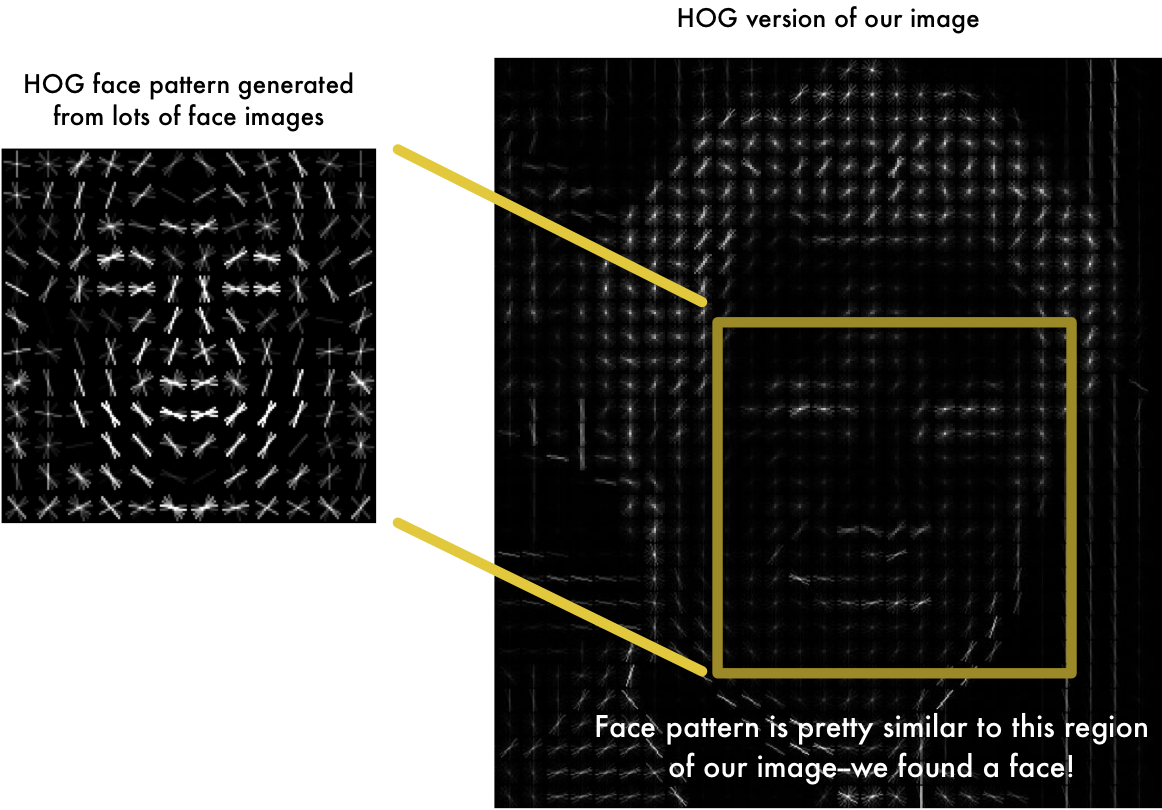
\includegraphics[width=100mm, keepaspectratio]{03_images/hog.png}
    \caption{HOG algoritmust demonstráló ábra \cite{artc_gold}.}
    \label{fig:hog}
\end{figure}

\subsubsection{Arcok orientációja}
Mivel egy valós környezetben az emberek nem mindig néznek a kamerába, így az arcukat különböző orientációkban, elfordulásokban rögzíti a kamera. Ezt figyelembevéve a „face-recognition” Python modul az arcokat transzformálja a feldolgozása során. Oly módon, hogy a szemek és az ajkak mindig ugyanazon helyen legyenek a képen. Ez megkönnyíti az arcok összehasonlítását.
Az arcok összehasonlításához a „face landmark estimation” algoritmust használja. Sokféle módja van két arc összehasonlításának ennek, de a modul a Vahid Kazemi és Joseph Sullivan által 2014-ben kifejlesztett megközelítést \cite{artc36} alkalmazza.
Az alapötlet, hogy definiálunk 68 specifikus pontot, ami minden arcon megtalálható. A pontokat a jellegzetes arcvonások mentén határozták meg, mint az áll, szemöldök, orr, ajkak és az arc körvonala, ahogyan a mellékelt \refstruc{fig:arcpontok} is szemlélteti.
\begin{figure}[!ht]
    \centering
    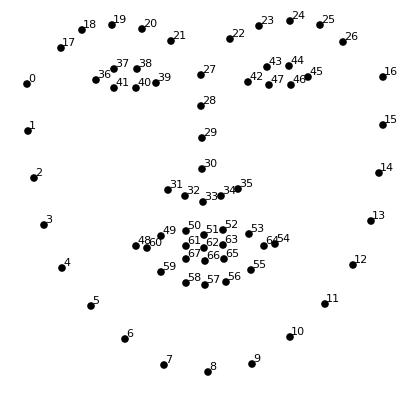
\includegraphics[width=75mm, keepaspectratio]{03_images/arcpontok.png}
    \caption{Arcot leíró jellegzetes pontok \cite{artc_gold}.}
    \label{fig:arcpontok}
\end{figure}

\subsection{3. lépés: arcok felismerése}
A felismerés lényege, hogy az emberi arcot leírjuk egy csak az egyénre jellemző módon. Kitétel, hogy az adattípus és formátuma összehasonlítható legyen az arcok között. A cél, hogy ugyanazt az arcot látva ez az adat megegyezzen, különböző arcok esetében pedig eltérőt kapjunk. Az emberek viselkedéséből kiindulva egy választás lehet a szem- vagy hajszín, arc formája, de ezek a paraméterek nem igazán értelmezhetőek egy számítógép számára, amely a kép egyes pixeleit vizsgálja. A kutatók rájöttek, hogy a legpontosabb megközelítés az, ha „hagyják”, hogy a számítógép maga találja ki az arcok összehasonlítását képező paramétereket és összegyűjtse ezeket az adatokat. Erre használt módszer a mély tanulás (deep learning), mely segítségével meghatározható, az arc mely részei fontosak a méréshez. A megoldás egy konvolúciós háló betanítása, amely minden egyes archoz meghatározott számú összehasonlítási pontot generál.

A korábban bemutatott Python-os „face-recognition” modul esetében, aminek Dlib az alapja egy 128 dimenziós vektort állít elő, ami részletesen leírja az arcvonásokat, az arc ismertető jegyeit. Ez a vektor alapján válik kvantálttá, gépi módon összehasonlíthatóvá az arc. A betanítás folyamat röviden leírva: gyakorló képeket biztosítunk a konvolúciós háló számára, melyekről megadjuk, hogy ki található rajtuk. Elvárjuk, hogy olyan 128 elemű vektort készítsen a képekről, melyek euklidészi térben értelmezve közel esnek egymáshoz (távolságuk minimalizálására törekszik), ha két azonos ember arcáról készültek. Távol esnek egymástól a vektorok, ha két különböző ember arcáról képet vizsgál. Megfelelő mennyiségű gyakorló képet biztosítva mély tanulás a háló paraméterei úgy módosulnak, hogy az előző két kitételt minél pontosabban hajtsa végre \cite{artc_gold}. Ezt a betínítást a „face-recognition” modul megalkotója már elvégezte, a \refstruc{sec:facerec}ban leírt pontosságot elérve.

\clearpage %Page break
\section{Hardveres tervezési szempontok}
\label{sec:sec-cam}
Mivel a Biscee robot már fel van szerelve az erre a célra megfelelő hardverrel, kettő BASLER acA1300-60gc kamerával (\refstruc{fig:cam}), így ez a feltétel már teljesült. Következő lépésként a kamera képéhez hozzá kell férni. A roboton futó ROS keretrendszer segítségével, melyet a \az+\refstruc{sec:inros}ben mutatok be, ez könnyen a megvalósítható. A ROS hasznos eszközöket biztosít a külső eszközök elérésére. A keretrendszeren belüli feldolgozáshoz egyértelmű választás volt az OpenCV Python nyelvre implementált modulja. A cél, hogy a feldolgozás valós időben dolgozzon, mert akkor ítélhető hasznosnak az információ, ha rögtön tudjuk kik vannak a robot látóterében. Emiatt fontos annak a csatorna sebességének az optimalizálása, amin keresztül eljut a kamerától az arcfelismerő kódban feldolgozhatóságig a kép. Szempontok, amiket tervezésnél nem lehet megkerülni: a gyorsaság, a minőség és a hardveres lehetőségek, azaz erőforrások használata.

\begin{figure}[!ht]
    \centering
    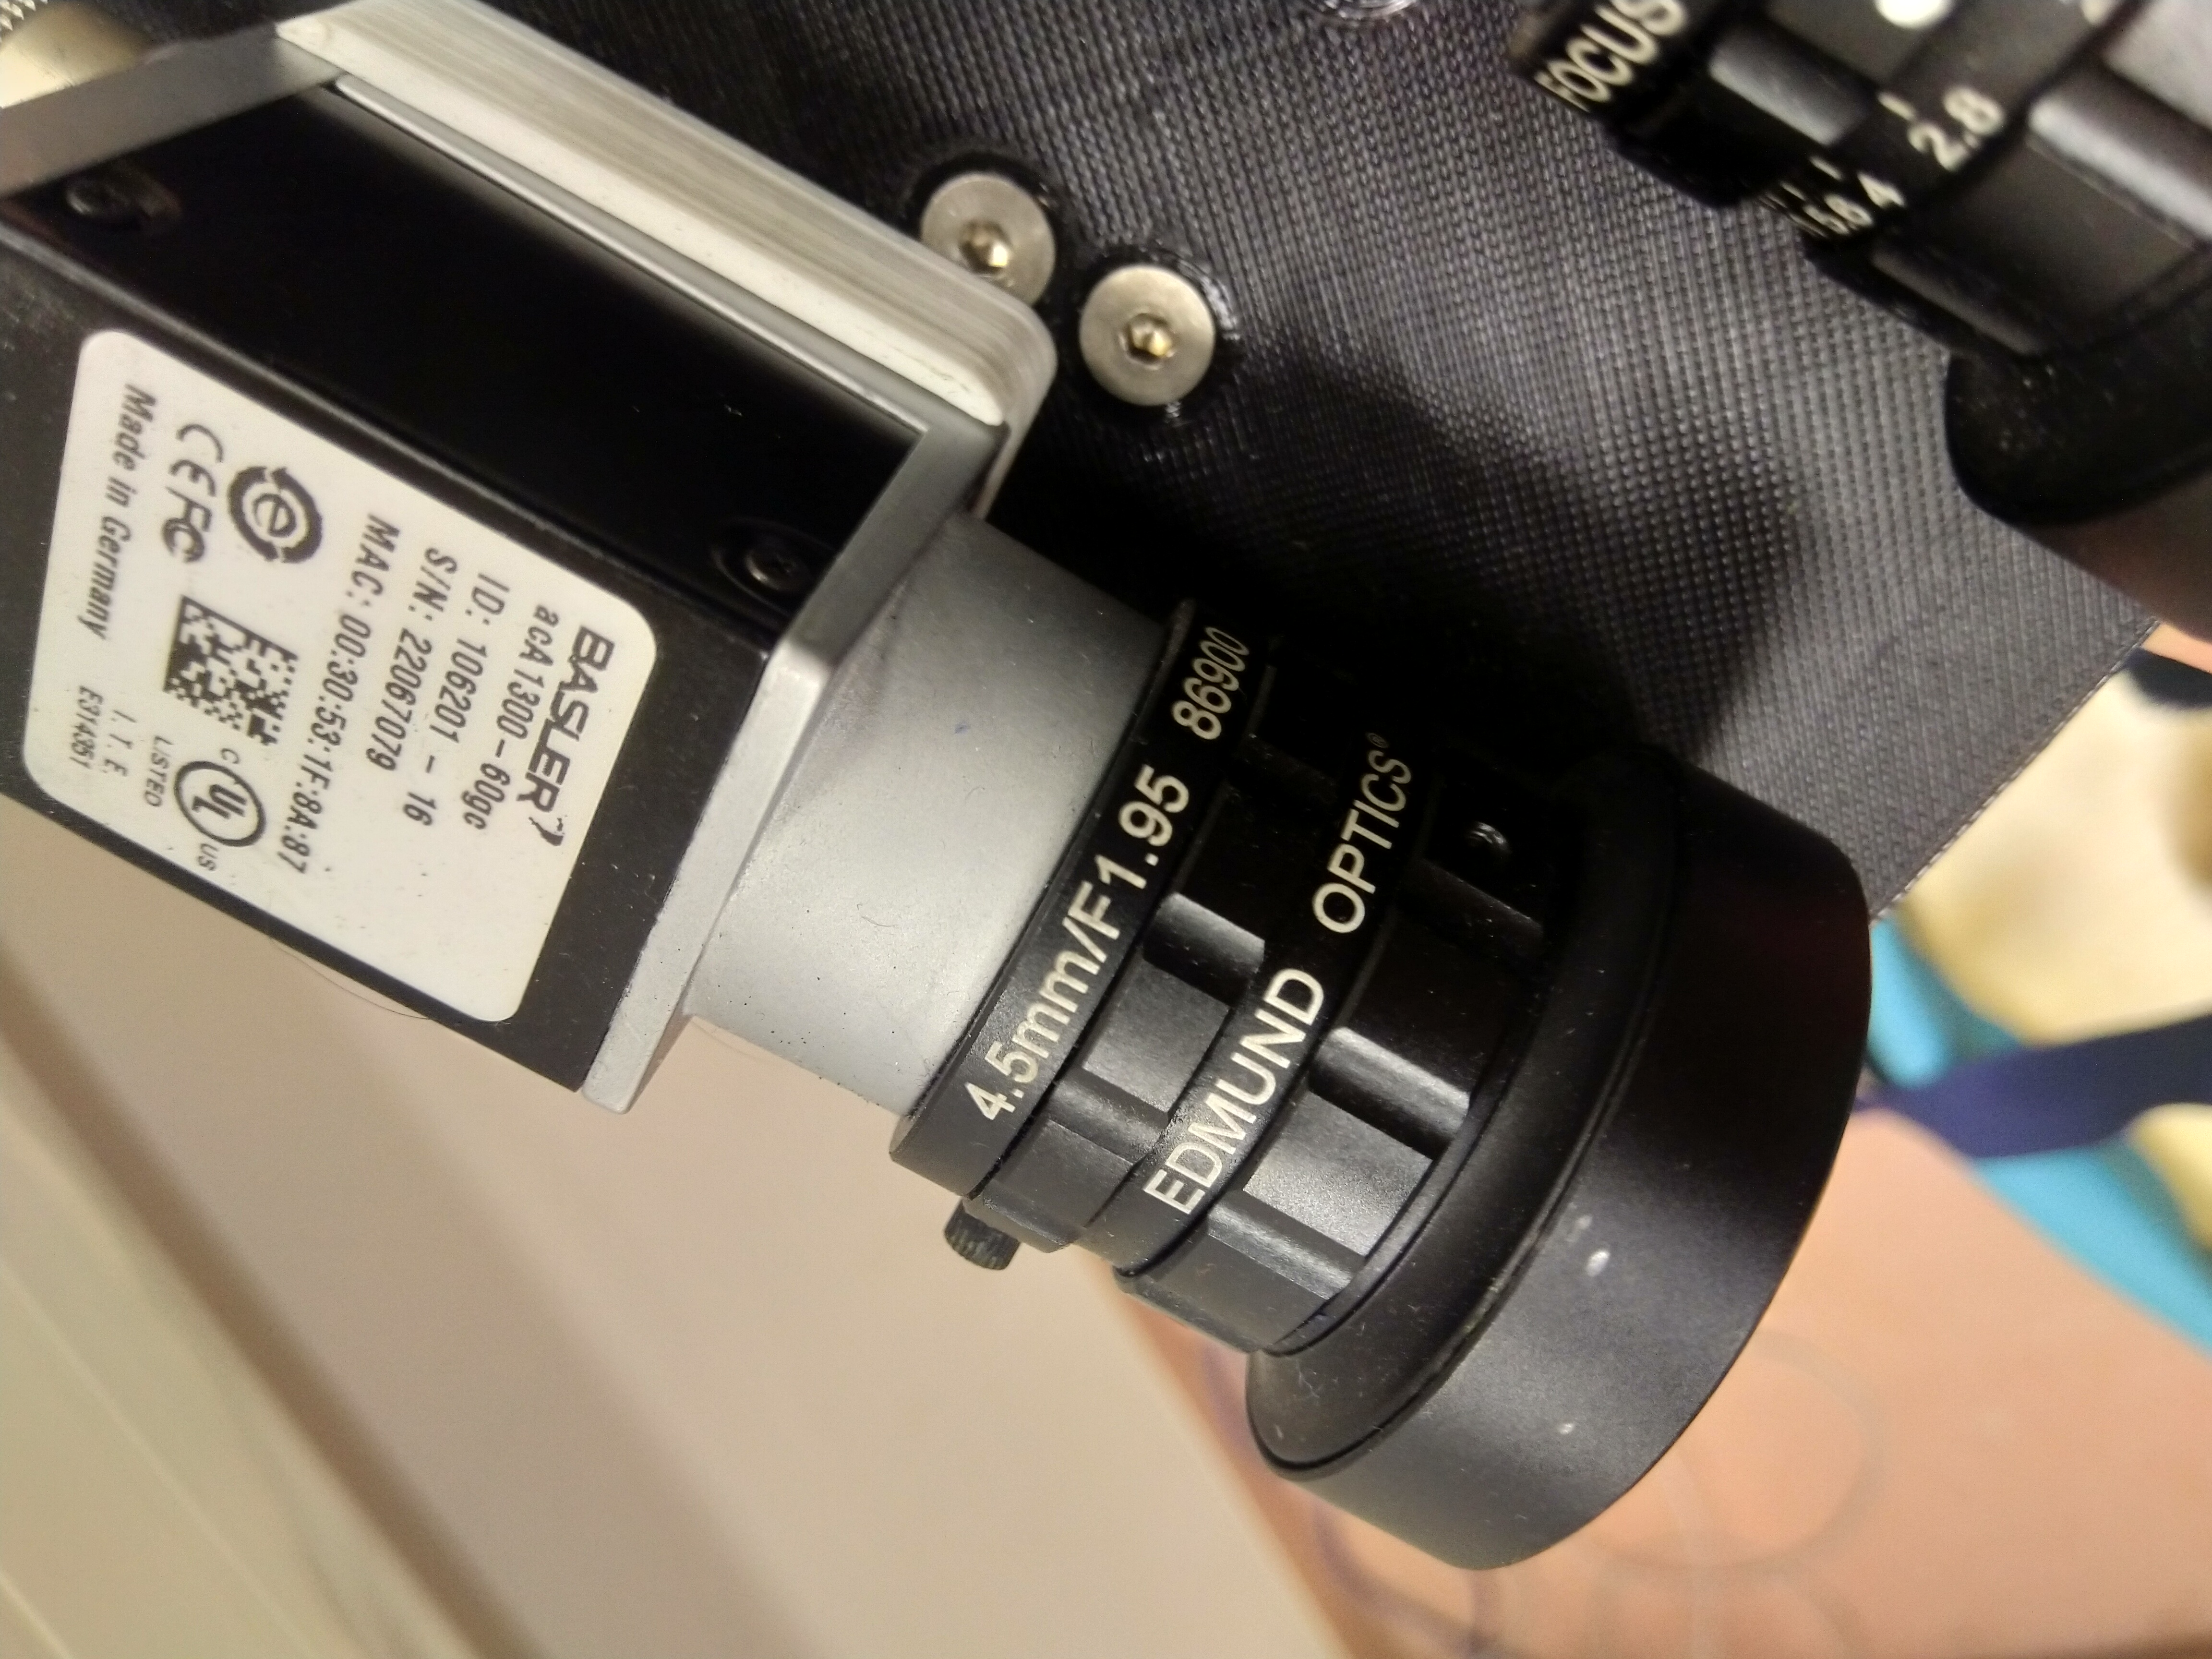
\includegraphics[width=80mm, angle=180, keepaspectratio]{03_images/kamera1.jpg}
    \caption{BASLER acA1300-60gc kamera.}
    \label{fig:cam}
\end{figure}

Ebben a fejezetben a paraméterek kapcsolatáról írok. Minél kevesebb időt szeretnénk feldolgozásra fordítani, annál erősebb hardver szükséges. Egyértelműen minél több erőforrást tudunk a feldolgozásra biztosítani, annál gyorsabb lesz a folyamat. Minél jobb minőséget (nagyobb felbontást) szeretnénk elérni, annál nagyobb a hardveres követelmény. A jobb minőség több információt jelent, amivel az algoritmusnak számolnia kell. Ebből kifolyólag több számítási kapacitásra van igény. A minőség (felbontás) és gyorsaság közötti kapcsolat már következik az előzőkből. Az erőforrásokban mindenképpen kompromisszumot kell kötnünk, ezért fontos, hogy megtaláljuk azt a minőséget, ami még megfelel az információ elérésére, de nem lassítja a folyamatot, oly módon hogy az információ elértéktelenedjen. Megállapítható, hogy ez egy szigorúan valós idejű rendszer, mivel az információ, ami jelen esetben az jelenti, hogy milyen arcokat ismert fel a robot, tehát kik azok a személyek akik a látóterében tartózkodnak, az idő elteltével elértéktelenedik. 
\chapter{Algoritmus elhelyezése ROS-ban}
\label{sec:inros}

Ebben a fejezetben leírom, hogyan helyeztem el a tervezett algoritmust ROS-on (Robot Operating System-en) \cite{ros} belül. Kitérek az ROS fejlesztési elveire, illetve az algoritmus leírásában használt kifejezésekre, melyek szükségesek a megértésben. Bemutatom a tervezett csomagot, elemeit és működését. Használt kommunikációs csatornákat, rétegeket és a felhasznált modulokat, könyvtárakat. A fogalmak bemutatásához az ROS dokumentációját \cite{ros} használtam alapul.

\section{ROS bemutatása}
A ROS (Robot Operating System) könyvtárakat és eszközöket biztosít, amelyek segítenek a szoftverfejlesztőknek robotokon alkalmazások létrehozásában. Hardveres absztrakciót, eszközillesztőket, könyvtárakat, megjelenítőket, üzenettovábbítást, csomagkezelést és még sok mást eszközt biztosít egy környezetben. A ROS nyílt forráskódú, BSD licensz\footnote{BSD licensz: \url{https://www.freebsd.org/copyright/freebsd-license/}} alatt van licencelve.

A ROS egy meta-operációs rendszer, mely olyan szolgáltatásokat is nyújt, amelyek egy operációs rendszerben eleve be vannak építve, beleértve a hardveres absztrakciót, az alacsony szintű eszközvezérlést, az általánosan használt funkciók megvalósítását, a folyamatok közötti üzenettovábbítást és a csomagkezelést. Megkönnyíti csomagok létrehozását és futtatását több számítógépen, ehhez eszközöket és könyvtárakat biztosít.

ROS-ban létrehozott számítási gráffal (Computation Graph) modellezhető kommunikációs kapcsolatok hálózata és „peer-to-peer" megvalósítása. Többféle kommunikáció valósítható meg ROS-on belül, szinkron kommunikáció formájában „service”-eken keresztül vagy aszinkron „topic”-okon keresztül. Adatok tárolását „parameter server”-en biztosítja.
A ROS célja, hogy a megírt kód újrafelhasználható legyen különböző kutatásokban, fejlesztésekben. Folyamatok alá egy elosztott keretrendszert biztosít. „Node”-ok hozhatók létre, ezek olyan egységek, melyek képesek információkat küldeni, fogadni vagy feldolgozni és továbbítani. A „node”-ok ROS-on belül elkülönült rendszereket alkotnak, a változókat külön képesek kezelni, de egymással meg is tudják azokat osztani. Ennek a felépítésnek előnye, hogy komplex a folyamatokat, rendszereket könnyen átlátható részekre lehet szétbontani.

\section{ROS keretrendszer elvei} %TODO ITT TARTOK 23:18
A készítők minimális tárhely igényre és az írt kódok felhasználók közötti megosztásának megkönnyítésére törekedtek, mely segíti az integrálást különböző robotokra tervezett keretrendszerekkel. A ROS-t már integrálták az OpenRAVE-vel, az Orocos-szal és a Player-rel. Pythonn és C++ programozási nyelven van lehetőség csomagok fejlesztésére. Tesztelést megkönnyíti a „rostest”: beépített tesztrendszer, amely aszisztál tesztek írásában és lebonyolításában. A ROS alkalmas nagy futásidejű rendszerek és hosszú fejlesztési folyamatok kivitelezéséhez.

\section{ROS-ban használt fogalmak}
Három szintre különíthető el a ROS felépítése\footnote{ROS concepts: \url{http://wiki.ros.org/ROS/Concepts}}: fájlrendszer (Filesystem level), számítási gráf (Computation Graph) és a közösség (Community) által fejlesztett csomagok szintje. A fájlrendszer szintű fogalmak főként a lemezen, tárhelyen található ROS erőforrásokra vonatkoznak. A Computation Graph a „node”-ok kapcsolata, gráfelméleti értelmezésében „node”-ok alkotják a gráf csomópontjait. Ebben a fejezetben e két koncepciós szint fogalmait mutatom be a dolgozat érdemi részének megértése céljából.

\subsection{ROS fájlrendszer}
\subsubsection{Csomagok}
A csomagok jelentik a szoftverek ROS rendszerben való rendszerezésének fő egységeit. Egy csomag tartalmazhat ROS futásidejű folyamatokat („node”-okat), ROS-tól függő könyvtárat, adatkészleteket, konfigurációs fájlokat vagy bármi mást, ami hasznosan össze van szervezve futtatáshoz. A csomagok a ROS legmagasabb szervezettségi szintjei, a legkomplexebb egység, amit összeállíthat és kiadhat egy fejlesztő, egy csomag.

%\subsubsection{Meta-csomagok}
%A meta-csomagok speciális csomagok, amelyek egymáshoz kapcsolódó csomagokat tartalmaznak. A meta-csomagokat használhatók verziók közötti kompatibilis megoldásához.

\subsubsection{Package manifest}
A manifest-ek a csomagok főkönyvtárában található (A \verb|package.xml|) fájlok, melyek meta adatokat adnak a csomagokról, beleértve a fejlesztő nevét, a csomag verzióját, leírását, licencinformációit, függőségeit és egyéb meta információkat, például a használt „exportált” csomagokat. A \verb|package.xml| csomagjegyzékek REP-0127-es\footnote{REP-0127: \url{https://www.ros.org/reps/rep-0127.html}} szabvány szerint vannak definiálva.

\subsubsection{Repository}
Egy repository az ugyanazon ROS verzióra készült csomagok gyűjteménye, egy projekthez tartozó csomagok összesége. Egy robothoz tartozó „repository” tartalmazza a működéséhez szükséges telepített és használt csomagokat.

\subsubsection{Üzenet „message” leíró fájlok}
A \verb|.msg| kiterjesztésű fájlokban kell definiálni az üzenetek leírását, a kommunikáció adatszerkezetét. Csomagonként lehet definiálni különböző \verb|.msg| fájlokat, általánosan a \verb|package/srv/MyServiceType.srv| elérési útvonalon. Egy csomagban definiált üzenet másik csomagban is hivatkozható és használható lesz, fordítás és megfelelő függőségek megadása után.

\subsubsection{Szolgáltatás „service” leíró fájlok}
A \verb|.srv|” kiterjesztésű fájlokban leírt szolgáltatások határozzák meg a kérések („request”) és válaszok („response”) adatstruktúráit. Általános elérési útvonaluk: \verb|package/srv/MyServiceType.srv|. Az üzenetekkel egyező módon, egy csomagban definiált „service”-ek másik csomagban is hivatkozhatóak és használhatóak lesz.

%TODO új oldal?
\subsection{Computation Graph}
ROS folyamatok „peer-to-peer" hálózata, amelyek együtt dolgoznak fel adatokat. A hálózatot leíró folyamatok kommunikációs hálójának rendszerezési fogalma a fájlrendszer feletti architekturális szinten a „Computation Graph”. A következő pontokban a gráfot alkotó elemeket mutatom be.

\subsubsection{Node-ok}
A „node”-ok vagy csomópontok, olyan folyamatok, amelyek számítást, adatfeldolgozást végeznek. ROS moduláris felépítésének egységei. „Node”-okba szokás csoportosítani a különböző feladatokat, például egy „node” felelős a térképezésért, egy másik pedig a motorok vezérléséért. ROS-ban „node”-okat írhatunk C++ nyelven „roscpp”\footnote{roscpp: \url{http://wiki.ros.org/roscpp}} vagy Python nyelven a „rospy”\footnote{rospy: \url{http://wiki.ros.org/rospy}} könyvtárak („ROS client library”-k) felhasználásával.

\subsubsection{ROS Master}
Egy „nameservice”, tárolja a gráf „node”-jainak információit, segítségével találják meg egymást a „node”-ok és tudnak üzeneteket küldeni, szolgáltatásokat hívni. A „ROS Master" névadási és regisztrációs szolgáltatásokat nyújt a ROS rendszer minden „node”-ja számára. Nyomon követi a „topic”-ok „publisher”-eit és „subscriber”-eit és „service”-eket. A „Master" szerepe az, hogy lehetővé tegye az egyes ROS „node”-oknak egymás helyének meghatározását. Miután ezek a csomópontok megtalálták egymást, „peer-to-peer" kommunikációval közölhetnek adatokat egymással. A „Master" biztosítja a „parameter server"-t is.

\subsubsection{Parameter Server}
Lehetővé teszi kulcs és adat párok tárolását, a „Master" része. Innen elérhetőek a paraméterek a „node”-ok számára. Ilyen paraméterek lehetnek a robot fizikai dimenziói, mozgásra képes alkatrészek rotációja, elmozdulása, csatlakozó pontok és a robothoz kapcsolt szenzorok koordinátái.

\subsubsection{Üzenetek - „messages”}
A „node”-ok üzenetek küldésével kommunikálhatnak egymással. Egy üzenet egy adatstruktúra, amely adattípust és annak elnevezését tartalmazza. A szabványos primitív típusok (\verb|int, bool, float, string|) támogatottak, csakúgy, mint ezen primitív típusok tömbjei. Az üzenetek tetszőlegesen is tartalmazhatnak beágyazott, a felhasználó által primitív tagokból definiált struktúrákat és azok tömbjeit.

\subsubsection{Topic-ok}
A „topic”-ok vagy témák, az üzenetek továbbítására használt csatornák küldő-fogadó (subscriber-publisher) szemantikával. Egy „node” úgy küld üzenetet, hogy közzéteszi azt egy adott „topic”-on. A „topic” egy név, amely az üzenet tartalmának azonosítására szolgál. Egy bizonyos típusú adat iránt érdeklődő „node” feliratkozhat a megfelelő „topic”-ra. Az adott „topic”-on minden publikált adat után meghívódik a feliratkozott „node”-ban egy „callback” függvény, amelyben feldolgozhatjuk a kapott adatot. Egy „topic”-nak több adója és feliratkozója lehet egyidejűleg, és egyetlen „node” több „topic”-on is közzétehet és feliratkozhat rá. Általában az adók és a feliratkozók nincsenek tudatában egymás létezésének. Az információtermelést leválasztják annak fogyasztásáról. Egy „topic”-ot egy virtuális üzenetbusznak tekinthetünk. Minden busznak van neve, és bárki csatlakozhat a buszhoz üzenetek küldése vagy fogadása céljából, amennyiben az adatcsomag típusa megfelelő.

\subsubsection{Szolgáltatások - „services”}
A „subscriber-publisher” kommunikációs paradigma „many-to-many" azaz többen publikálhatnak a csatornára és többen is elérhetik az adatot, ezzel szemben a szolgáltatások két „node” között teremtenek kommunikációs csatornát. A modell: kérés-válasz (request-reply), azaz egy szerver „node” bizonyos név alatt egy szolgáltatást biztosít, amit egy másik „node”-on belül meg tudunk hívni. A hívás következtében a szerverként működő „node” meghív egy függvényt, így tekinthető távoli eljáráshívásnak. A hívó „node” megvárja a választ, ezzel megakasztva belső működését.

\section{ROS verzió}
ROS-ból léteznek disztribúciók, amik különböző fő verziókat jelentenek, ezekbe csoportosítva a ROS csomagokat. A disztribúciók célja, hogy lehetővé tegyék a fejlesztőknek, hogy egy stabil kódbázissal dolgozzanak mindaddig, amíg készen nem állnak az új verzióra való átállásra. Disztribúciók kiadása után korlátolt mértékben hibajavítások még fejlesztésre kerülnek hozzájuk, de jellemzően semmi olyan frissítést nem adnak ki a ROS fejlesztői, ami eltörné a kommunikációt azonos disztribúcióra írt csomagok között. A disztibúciók kiadása a Linux Ubuntu operációs rendszer fő verzióinak kiadását követi.

A Biscee roboton jelenleg futó csomagok nagy része ROS Melodic\footnote{ROS Melodic Morenia: \url{http://wiki.ros.org/melodic}} verzió alatt lett fejlesztve. Mivel csak a Python 2-es verziója használható csomagok fejlesztésére ez a verzió alatt, ezért kénytelen voltam ROS Noetic-et\footnote{ROS Noetic Ninjemys: \url{http://wiki.ros.org/noetic}} használni, ami már támogatja a Python 3-at, ami elengedhetetlen az OpenCV használatához. A különböző verziók közötti átjárásra már vannak létező megoldások, ezért nem limitálja az algoritmus használatát a roboton.

\section{ROS node-ok és kommunikációjuk}
A „node”-ok A ROS számítást végző egységei. Kombinációjuk gráfot alkot (Computation Graph) és „topic”-okon vagy „service”-eken keresztül kommunikálnak egymással. A cél, hogy egy „node” egy kiosztott feladatot lásson el, elszeparálva ROS-on belül a robothoz szükséges folyamatokat kisebb egységekre. Ennek előnye, hogy segíti a hibakeresést, egy-egy feladat felülvizsgálatához vagy lecseréléséhez elég az ezt specifikusan ellátó „node” vizsgálata, ismerete. Az esetleges hibák izolálva vannak „node”-okon belül így egy „node” leállása nem hat ki a robot teljes működésére, nem gátolja a többi „node” operációját. Megosztott feladatok miatt az egy helyre leírt kód mennyisége is csökken, ami átláthatóbbá teszi fejlesztői oldalról. Nem jelent problémát a különböző nyelven írt „node”-ok közötti kommunikáció sem, a ROS által biztosított komminkációs módok képesek áthidalni. Például egy „node” kezeli a lézeres távolság mérést, egy másik a motorok irányítását, külön „node”-ban implementálhatóak csak a lokalizációhoz tartozó feladatok és így tovább. A mintát követve, könnyen bővíthető és fejleszthető egy robot funkciókészlete.
Minden „node” rendelkezik egy névvel, ami egyedileg azonosítja a gráfban. ROS-ban „node”-okon belül egy programozási nyelv használható (Python vagy C++), melyekhez két könyvtár áll a fejlesztők rendelkezésére: „rosccp" és „rospy". Mivel a csomagot Python nyelven fejlesztettem, ezért a következő két szakaszban (\refstruc{sec:ros_sp1} és \refstruc{sec:ros_s2}) a „rospy" könyvtár által biztosított ROS architektúrába illeszkedő kommunikációs módokról írok.

\subsection{Subscriber-publisher modell}
\label{sec:ros_sp1}
% http://wiki.ros.org/rospy/Overview/Publishers%20and%20Subscribers
Aszinkron kommunikációs forma, röviden „Pub/Sub" minta, amit a szerver nélküli vagy mikroszolgáltatás architektúrákban használnak. Két elemből áll: egy küldő / „publisher” és egy fogadó / „subscriber”. A publisher elküldi az üzenetet, a subscriber fogadja. A modell két előnye, hogy segíti a kommunikációban résztvevő egységek független működését és használható eseményvezérelt programozásra. Ahogyan a \refstruc{fig:pubsub} is szemlélteti, a publisher-ek aszinkron módon küldhetnek üzenetet a csatornára, ami a megérkezésüknek megfelelő sorrendben a subscriber-ek részére elérhető. Az összes subscriber, ami ugyanarra a „topic”-ra van feliratkozva látja az összes publikált üzenetet. Az üzenet eljuttatása azonnal megtörténik, amint felkerült a „topic”-ra, ez különbözteti meg a hagyományos üzenetközvetítési modellektől, ahol a felhasználónak vagy szolgáltatásnak kell lekérnie az üzenetet. A „Pub/Sub" elgondolás elszigeteli a csatorna két oldalán levő „publisher"-eket a „subscriber"-ektől, azaz nem tudnak egymás létezéséről. Javítja ezzel az alkalmazás biztonságát. Aszinkronitása segíti a nagy forgalom melletti folyamatos működést. Az egységek (ROS esetében „node”-ok) közötti „Pub/Sub" modellben az üzeneteket egy „buffer”-be gyűjti, és a „buffer”-t minden „subscriber" kimenetére eljuttatja. Megadható a „buffer” mérete, vagyis hány üzenet eltárolására legyen alkalmas. Ennek megválasztása függ a használat céljától. Ha egy üzenetet meghatározott frekvencián küldünk, akkor célszerű akkora „buffer” méretet választani, ami a frekvenciához jól társul. Ha változó időközönként küldünk egy vagy több üzenetet célszerű nagyméretű „buffer”-t megadni. A „topic”-on közölt üzenetek adatmodelljét \verb|.msg| fájlokban lehet megadni, amiket aztán lefordít „roscpp"-ben és „rospy"-ban elérhető osztályokra \cite{pubsub1}\cite{pubsub2}.
\begin{figure}[!ht]
    \centering
    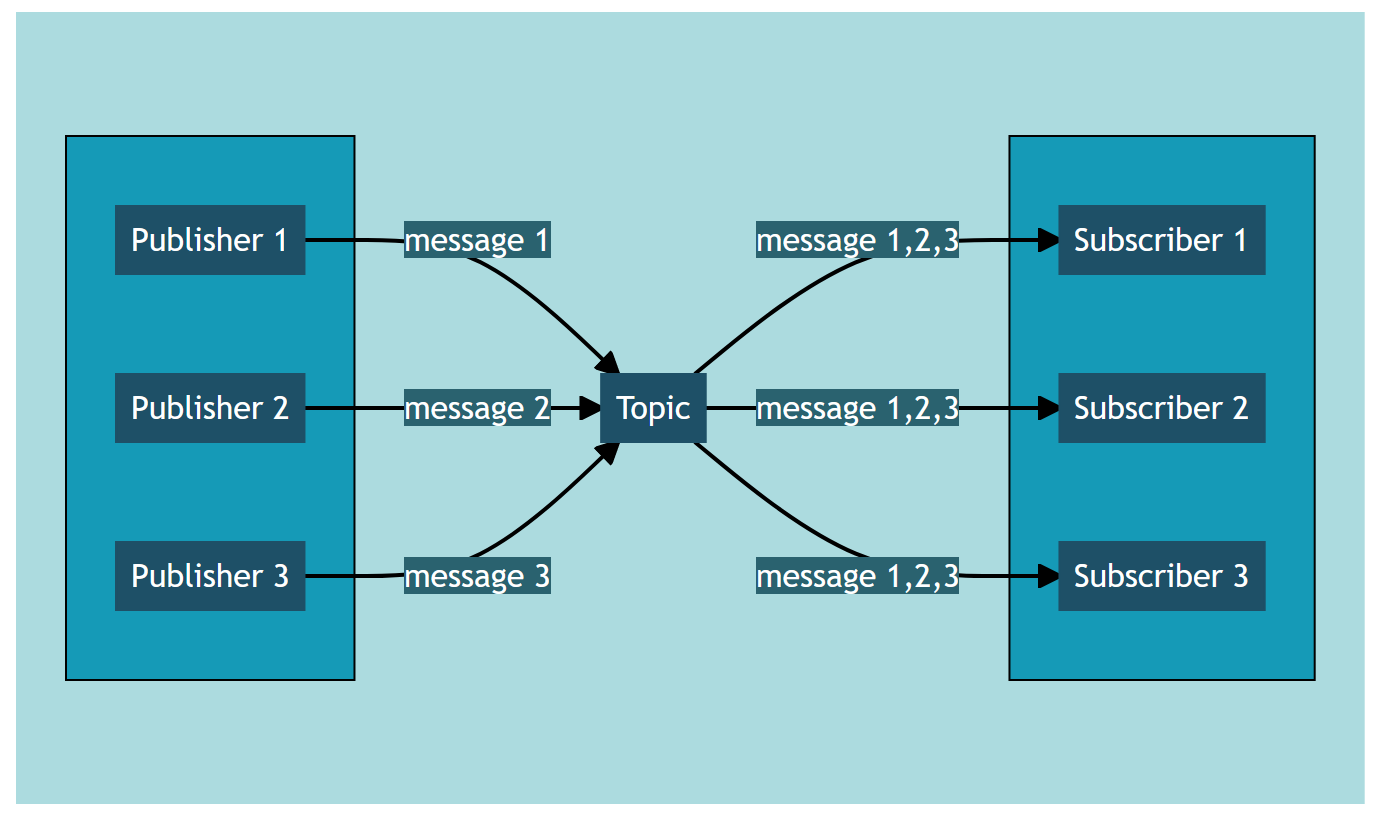
\includegraphics[width=150mm, keepaspectratio]{02_mermaid/mermaid02_pubsub.png}
    \caption{Publisher-subscriber modell.}
    \label{fig:pubsub}
\end{figure}
 \clearpage
\subsection{Service-request modell}
\label{sec:ros_s2}
% TODO forrás: http://wiki.ros.org/ROS/Tutorials/WritingServiceClient%28python%29
% https://learn.microsoft.com/en-us/azure/architecture/patterns/async-\verb|”request”|-reply
A szolgáltatások azaz „service"-ek egy másik mód a gráf „node”-jainak (csomópontjainak) kommunikációjára. A „service"-ek hívás-válasz (call-and-response) modellen alapulnak. Különbség a „topic”-okon való kommunikációval ellentétben, hogy csak akkor történik adatátadás, amikor egy kliens kifejezetten meghívja. Típusuk leírását \verb|.srv|” fájlban tehetjük meg, ami az üzenetek mintájára lefordul és utána hivatkozható lesz. Ugyanakkor az üzenetekhez képest két részből állnak: egy kérésből (request) és egy válaszból (response). A szolgáltatások meghívása szinkron történik. A kliens elindítja a „request”-et a szerver felé, mire a szerverben egy megadott „callback” függvény fut le. A futásidejétől függetlenül a kliens addig vár, amíg nem kapott valamilyen visszatérési értéket, amit a „response” tartalmaz. Amiben különbözik a „Pub/Sub” modelltől, hogy szinkron, azaz amíg a kliens a hívásra vár blokkolja a program futását. Célszerű olyan esetekben alkalmazni, amikor fontos információra vagy adatra van szükségünk. Ha a szolgáltatás meghívása után fel szeretnénk dolgozni az információt, vagy használni szeretnénk akkor előnyös, hogy megakasztja a futást a „response” beérkezéséig, s amint megérkezett az adat engedi, hogy fusson tovább a kód.
\begin{figure}[!ht]
    \centering
    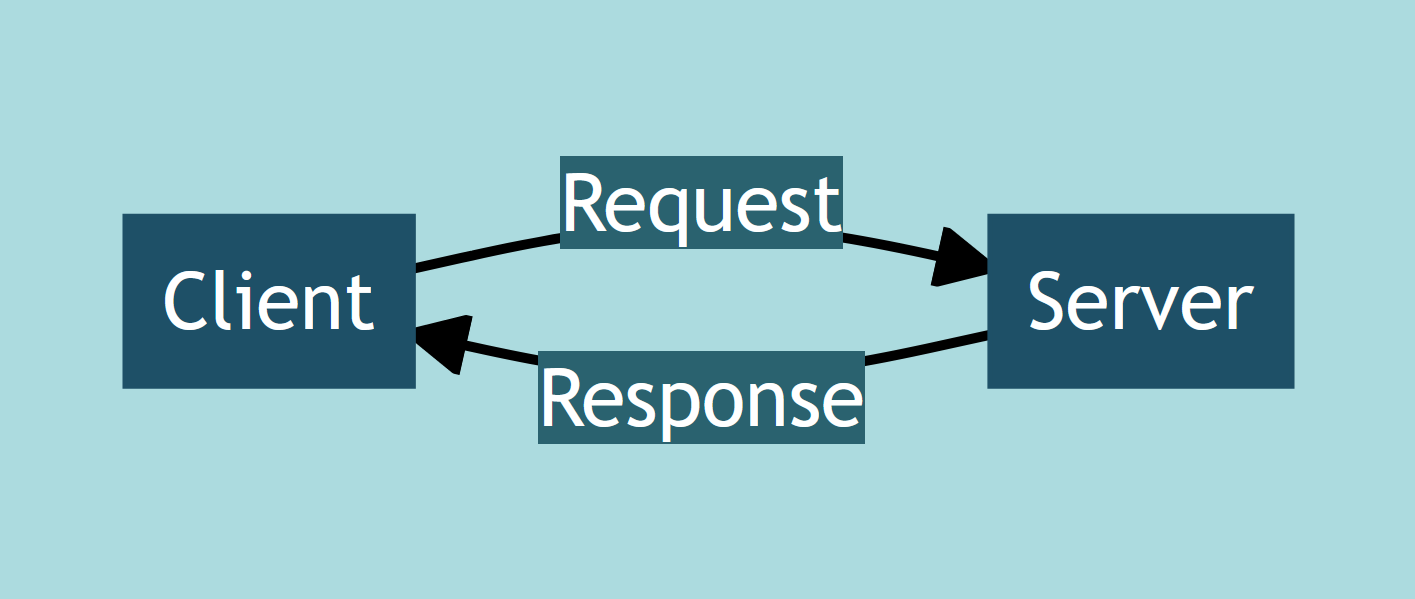
\includegraphics[width=100mm, keepaspectratio]{02_mermaid/mermaid03_service.png}
    \caption{Service-request modell.}
    \label{fig:service}
\end{figure}


\clearpage
\section{Tervezett csomag}
Ebben a fejezetben egy áttekintést biztosítok, milyen elemek alkotják az általam létrehozott csomagot. Leírom a ROS mellett használt fontos modulok működését, „node”-ok be- és kimeneteit alkotó „subscriber”-ek és „publisher”-ek és a bennük létrehozott változók, illetve függvények, melyek működésük megértésének szempontjából fontosak.

\subsection{Elhelyezés ROS-on belül}
ROS keretrendszer alapelveibe illeszkedően egy csomagot hoztam létre, ennek előnye, hogy bármilyen roboton, melyen ROS fut könnyen telepíthető. A csomag három „node”-ból áll. A külön „node”-ok létrehozása segíti a különböző folyamatok csoportosítását és az erőforrások felhasználásának ütemezését. A „node”-ok párhuzamosan futnak egymás mellett és „topic”-okon, illetve „service”-eken keresztül kommunikálnak egymással. A három „node” az alábbi ábrán látható (\refstruc{fig:fullmin}). A kamera képének elérésére készített „node” az OpenCV Python nyelvre készített csomagját\footnote{opencv-python: \url{https://pypi.org/project/opencv-python/}} használja. Az arcfelismerés fő folyamatára „Face recognition node” szolgál. Hozzá kapcsolódva egy külön \verb|ImageProcessor| osztályba szerveztem ki a kép feldolgozásával kapcsolatos feladatokat, mint az arcok észlelése és a felismert arcok megjelölése. A „Face database node” a \verb|DatabaseManager| osztályt használva kezeli és tárolja az adatokat. Az utolsó két „node” közösen támaszkodik a \verb|DataInterface| osztályra, az adattípusok közötti fordítások, átalakítások elvégzésében.

\begin{figure}[!ht]
    \centering
    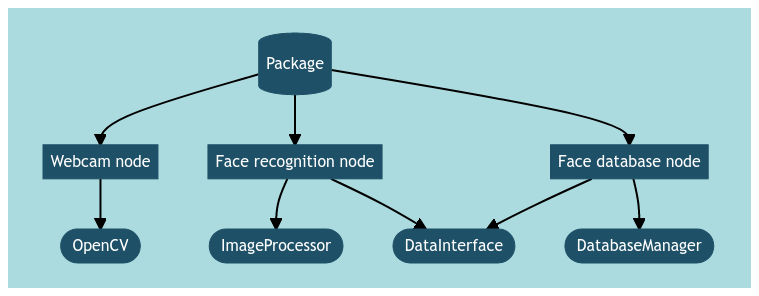
\includegraphics[width=150mm, keepaspectratio]{02_mermaid/mermaid01_minimal.png}
    \caption{Csomag belső kommunikációs csatornái.}
    \label{fig:fullmin}
\end{figure}

\clearpage
\subsection{Felépítés}
A három „node”-ot a csomag \verb|scripts| mappájában helyeztem el, alkalmazkodva a ROS-ban általánosan használt fájlrendszer kialakításhoz. Ezeket a „node”-okat: \verb|image_publisher.py|,  \verb|face_recognition_core.py| és \verb|face_database.py| fájlokban implementáltam. A ROS kétféle könyvtárat biztosít: „rospy” és „roscpp”, Python és C++ nyelvekhez. A fájlnevek kiterjesztéséből (.py) is látható, hogy python nyelven fejlesztettem. A választásom fő indoka, hogy ezen a nyelven van a legtöbb programozói tapasztalatom. További indoklás, hogy a Biscee roboton eddig alkalmazott csomagok nagy része is ezen a nyelven íródott, így fontos, hogy architekturálisan illeszkedjen ebbe a környezetbe, megkönnyítve a többi felhasználó és fejlesztő munkáját. Továbbá a használt „face-recognition" könyvtár is python nyelvben készült, ezért egyértelmű volt a választás.
\begin{figure}[!ht]
    \centering
    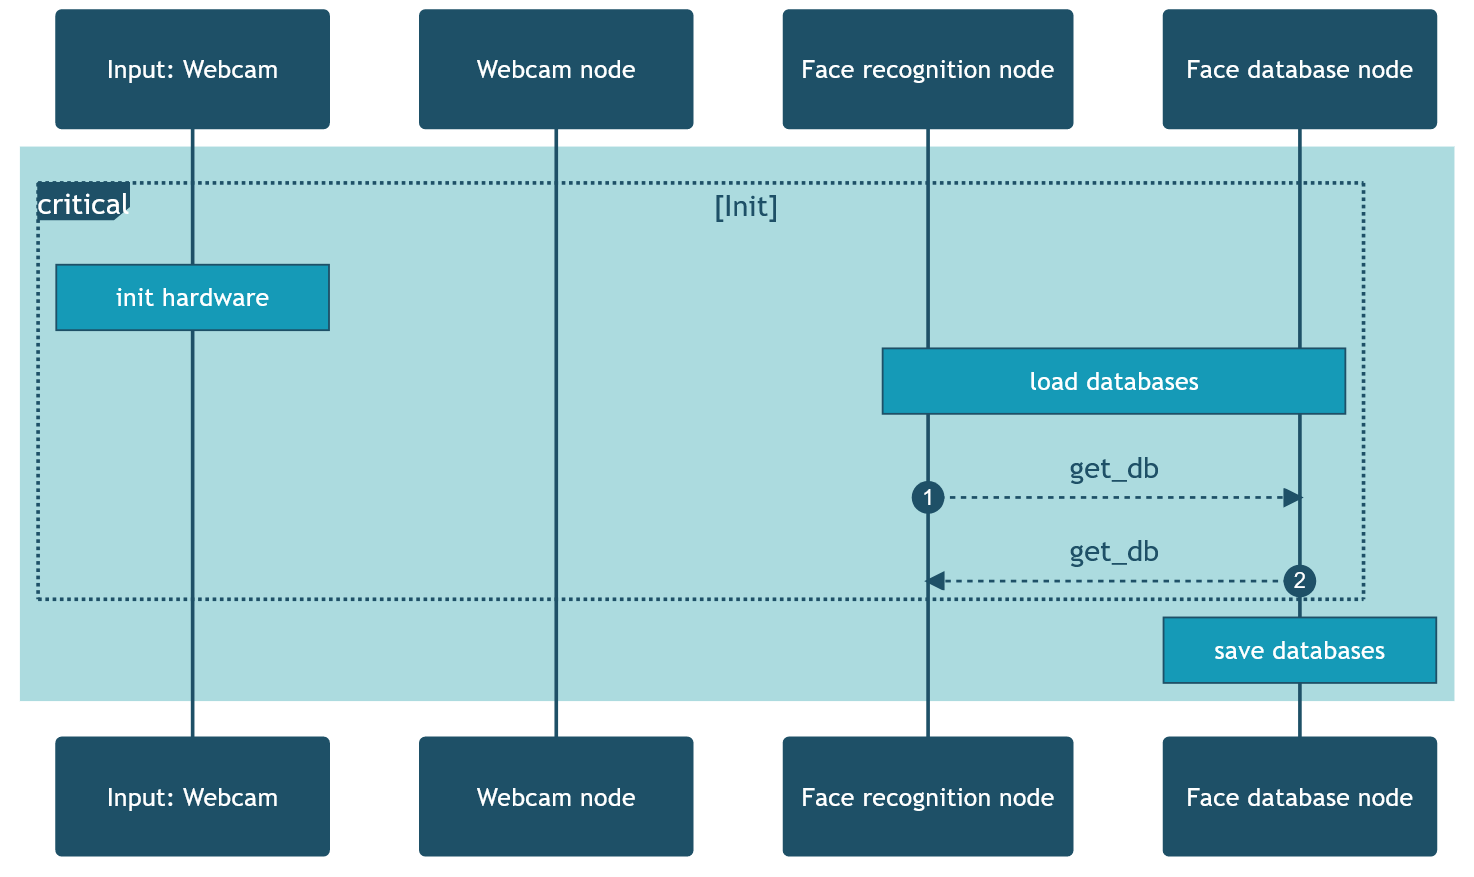
\includegraphics[width=155mm, keepaspectratio]{02_mermaid/full_init2.png}
    \caption{Csomag belső kommunikációs csatornái inicializáláskor.}
    \label{fig:fullcomm1}
\end{figure}
%TODO: részletes leírás a képről

A kommunikációs csatornák ábrázolása a „node”-ok, ki- és bemenetek között: inicializálás közben (\refstruc{fig:fullcomm1}) és működés közben (\refstruc{fig:fullcomm}). Működés közben használt „topic”-okat folytonos vonallal, a „service"-eket szaggatott vonallal ábrázoltam. Az inicializálás és működés közbeni kommunikációt a \refstruc{sec:modules}ban taglalom „node”-okra bontva.

A csomagot (\refstruc{fig:fullcomm}), mint rendszert úgy terveztem, hogy egy bemenettel és egy kimenettel rendelkezzen. A bemeneti információ, amire szükség van egy élő kamera kép. A célroboton már létezik egy „node”, ami képes ennek az információnak a biztosítására, de a saját csomagom írása közben nem volt lehetőségem a roboton fejleszteni, illetve a fentebb említett célom, ami a ROS egyik elve, hogy a csomag használható legyen bármilyen roboton (feltéve, hogy kompatibilis a verzió és a hardware-es, szoftveres feltételek ki vannak elégítve). Ez okból kifolyólag írtam egy saját „node”-ot, aminek az a feladata, hogy csatlakozzon a látást biztosító kamerához, és ennek a képét továbbítsa a csomagban létrehozott többi „node” számára, melyek elvégezhetik ennek a bemenetnek a feldolgozását, majd segítségévél az arcfelismerést és a hozzá tartozó feladatokat.

\begin{figure}[!ht]
    \centering
    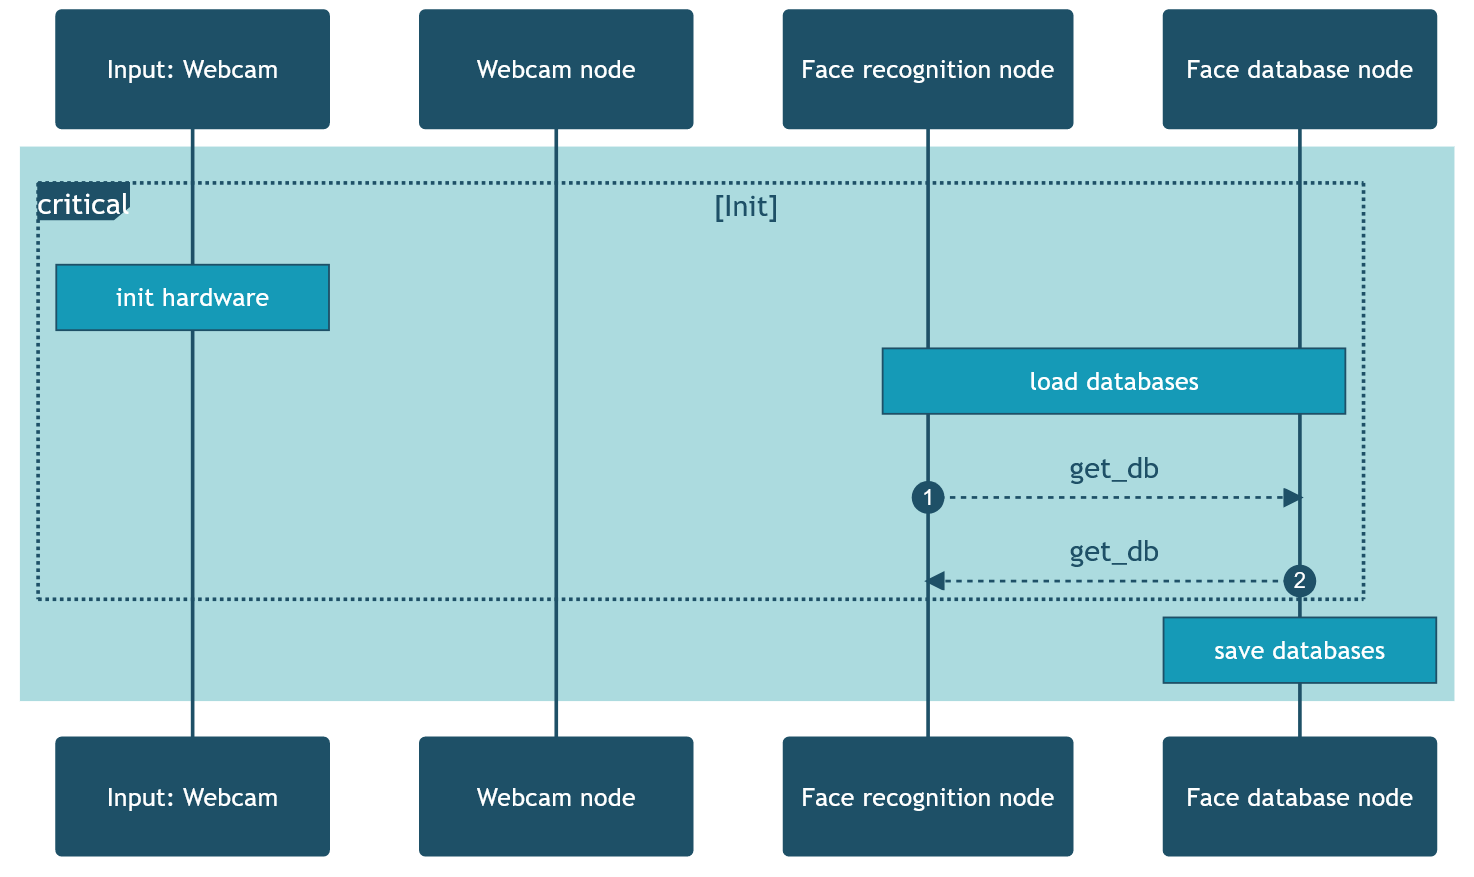
\includegraphics[width=155mm, keepaspectratio]{02_mermaid/full_init2.png}
    \caption{Csomag belső kommunikációs csatornái részletesen.}
    \label{fig:fullcomm}
\end{figure}

\clearpage
\section{Csomag moduljai}
\label{sec:modules}
    \subsection{Kamera kezelését végző node}
Az \verb|image_publisher.py| fájlban található „node” feladata, hogy a robothoz csatlakoztatott kamera élő képen Opencv-python modul segítségével végez egy elő feldolgozást, majd továbbítja a kép teljes feldolgozását, az arcok felismerését végző „node” számára.
\begin{figure}[!ht]
    \centering
    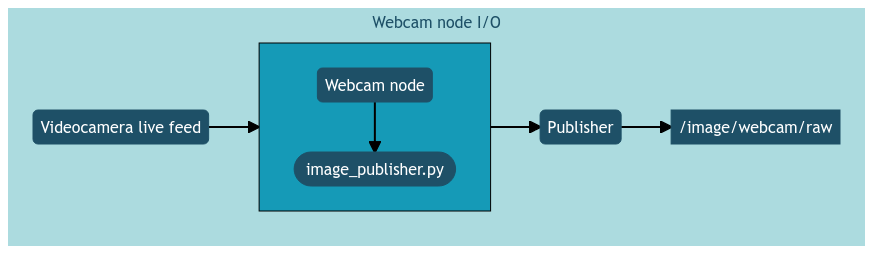
\includegraphics[width=125mm, keepaspectratio]{02_mermaid/mermaid10_wc_io.png}
    \caption{Kamera kezelő „node" „I/O"-ja.}
    \label{fig:wcio}
\end{figure}

Opencv-python modul (továbbiakban csak cv2), a nyílt forráskódú OpenCV projekt Python programozási nyelvre készült könyvtára számítógépes látáshoz, képfeldolgozáshoz. A cv2 \verb|VideoCapture| osztályának segítségével olvassa be a csatlakoztatott kamera képét, itt megadhatóak paraméterek, melyek közvetlenül befolyásolják a kiolvasott kép felbontását, enkódolását és a kiolvasás sebességét. Ezt követően a beolvasott képet át kell alakítani ROS „topic”-on publikálható formátumú üzenetté. A folyamatot a \refstruc{fig:wcp} szemlélteti. A publikálás elvégzéséhez a \verb|cv_bridge| modul segít. A modul, mint a nevéből is következik hidat biztosít a cv2-vel beolvasott kép és a ROS-ban publikált üzenet formátuma között. Az átalakítást követően az üzenetet a \verb|/image/webcam/raw| „topic”-on publikálja.
\begin{figure}[!ht]
    \centering
    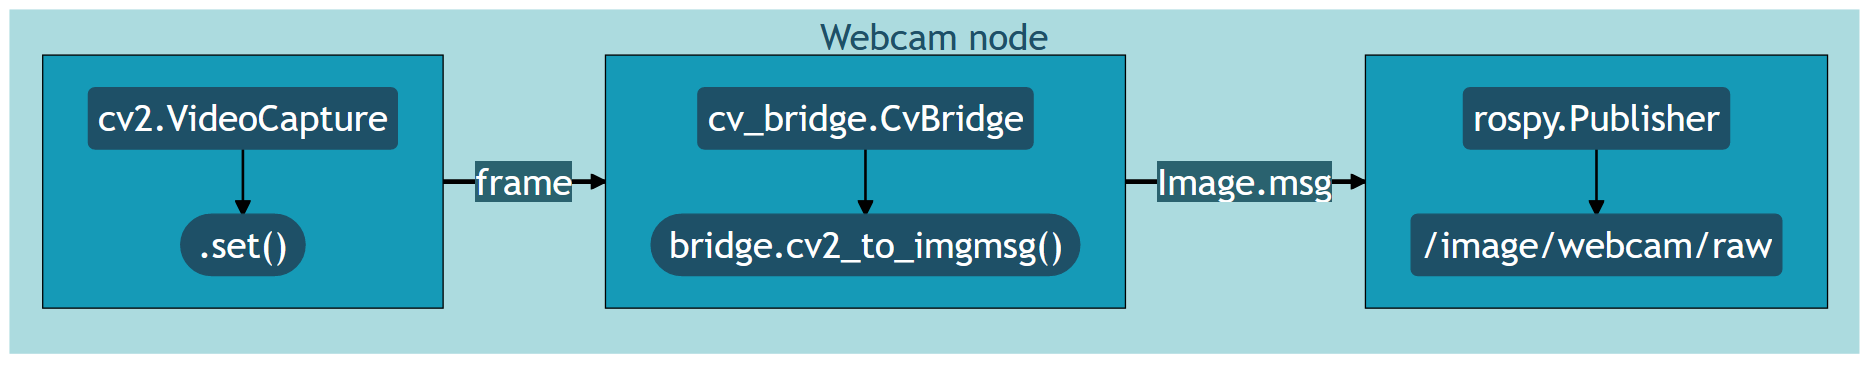
\includegraphics[width=150mm, keepaspectratio]{02_mermaid/webcam_node3.png}
    \caption{Kamera kezelő „node" folyamatábrája.}
    \label{fig:wcp}
\end{figure}

A „topic” elnevezése az általános ROS szokásjogot követi, amelyik üzenet egy képnek valamilyen enkódolását tartalmazza \verb|/image| nevű „topic”-ra kerül, ezen belül megnevezve mi a kép forrása, ami jelen esetben fejlesztés közben egy webkamera volt, illetve utólag megjelölve „raw”, aminek jelentéstartalma, hogy ez a kép teljes egészében, amit a kamera lát. Tehát még nincsenek rárajzolva az emberek arcát jelölő négyzetek és neveik.

\subsection{Arcfelismerést végző node}
Ez a „node” alkotja a csomag magját, ez a legfontosabb része, a \verb|face_recognition_core.py| fájlban implementáltam. Itt történik az emberek észlelése és azonosítása. A kommunikációhoz használt csatornáit a \refstruc{fig:frio} jeleníti meg.
%\begin{figure}[!ht]
%    \centering
%    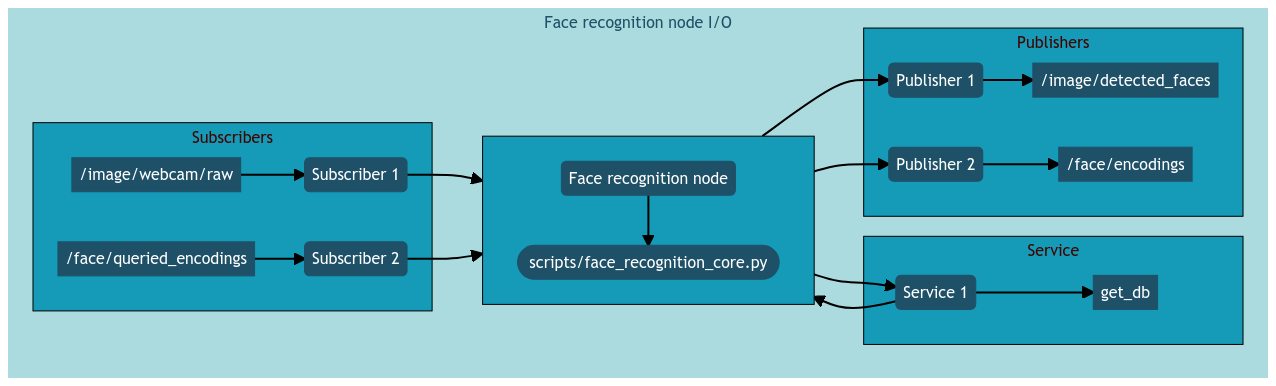
\includegraphics[width=150mm, keepaspectratio]{02_mermaid/mermaid20_fr_io.png}
%    \caption{Arcfelismerést végző „node" „I/O"-ja.}
%    \label{fig:frio}
%\end{figure}
%TODO: ábraleírás van ennyi annyi subja pubja mik a topicok

\subsubsection{Bemenetek}
Arcfelismerést végző „node” három bemenettel rendelkezi (\refstruc{fig:fri}). Az első „subscriber" feliratkozik a \verb|/image/webcam/raw| „topic"-ra, ahonnan megkapja a kamera képét \verb|image.msg| formátumban, amit a \verb|CvBridge| osztály \verb|.imgmsg_to_cv2()| függvénye alakít át felhasználható, elemezhető adattá. A második „subscriber" az adatbázist kezelő „node" által indított kommunikáció fogadására szolgál. Általam definiált \verb|Encodings.msg| formátumban megkapott adatokat a szintén általam írt \verb|DataInterface| osztály \verb|.msg2enc()| függvénye fordít a „node"-ban futó kód működéséhez szükséges formátumúvá. A „subscriber"-ek mellett kliensként is működik, a \verb|get_db| „service"-en keresztül kéri le az adatbázist kezelő „node"-tól az adatokat, itt szintén szükséges egy átalakítás, mint a második „subscriber"-ről érkező adatok fogadása során. Az alsó ábrán (\refstruc{fig:fri}) látható, hogy a \verb|DataInterface| osztály által átalakított adatok milyen formátumúak.
\begin{figure}[!ht]
%TODO szétdarabolni az ábrát NEM
    \centering
    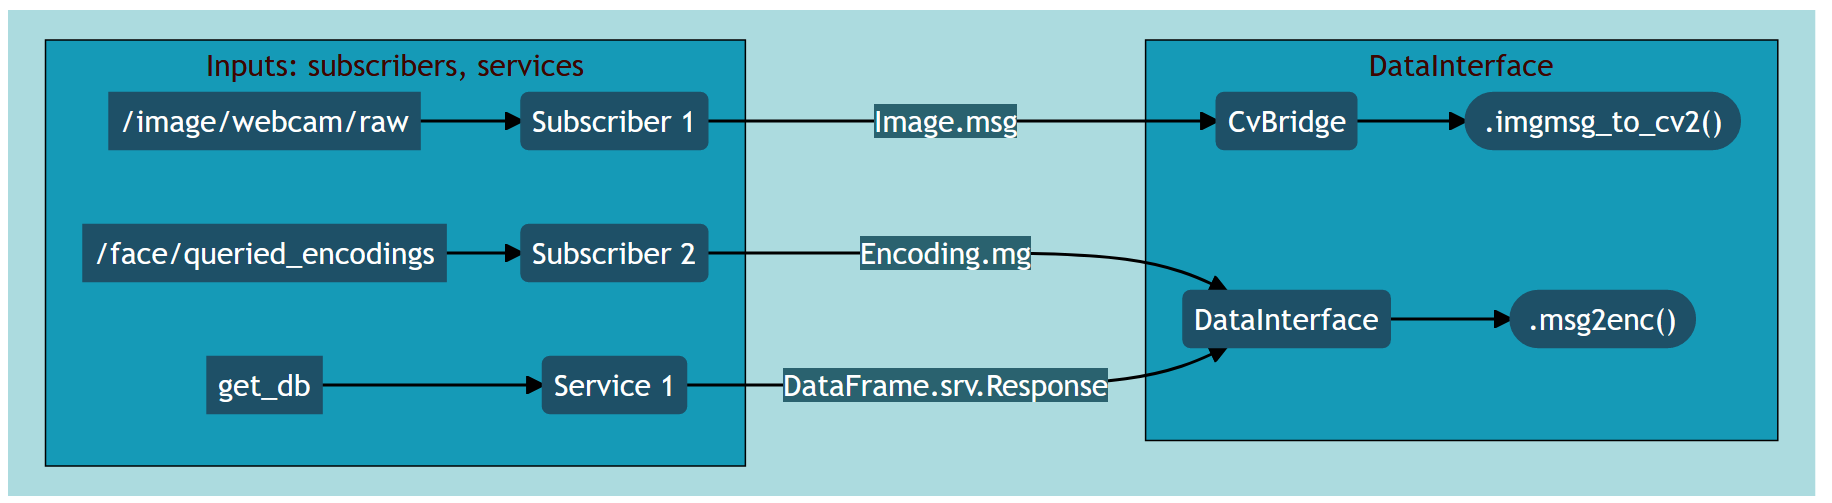
\includegraphics[width=150mm, keepaspectratio]{02_mermaid/fr_bemenet1.png}
    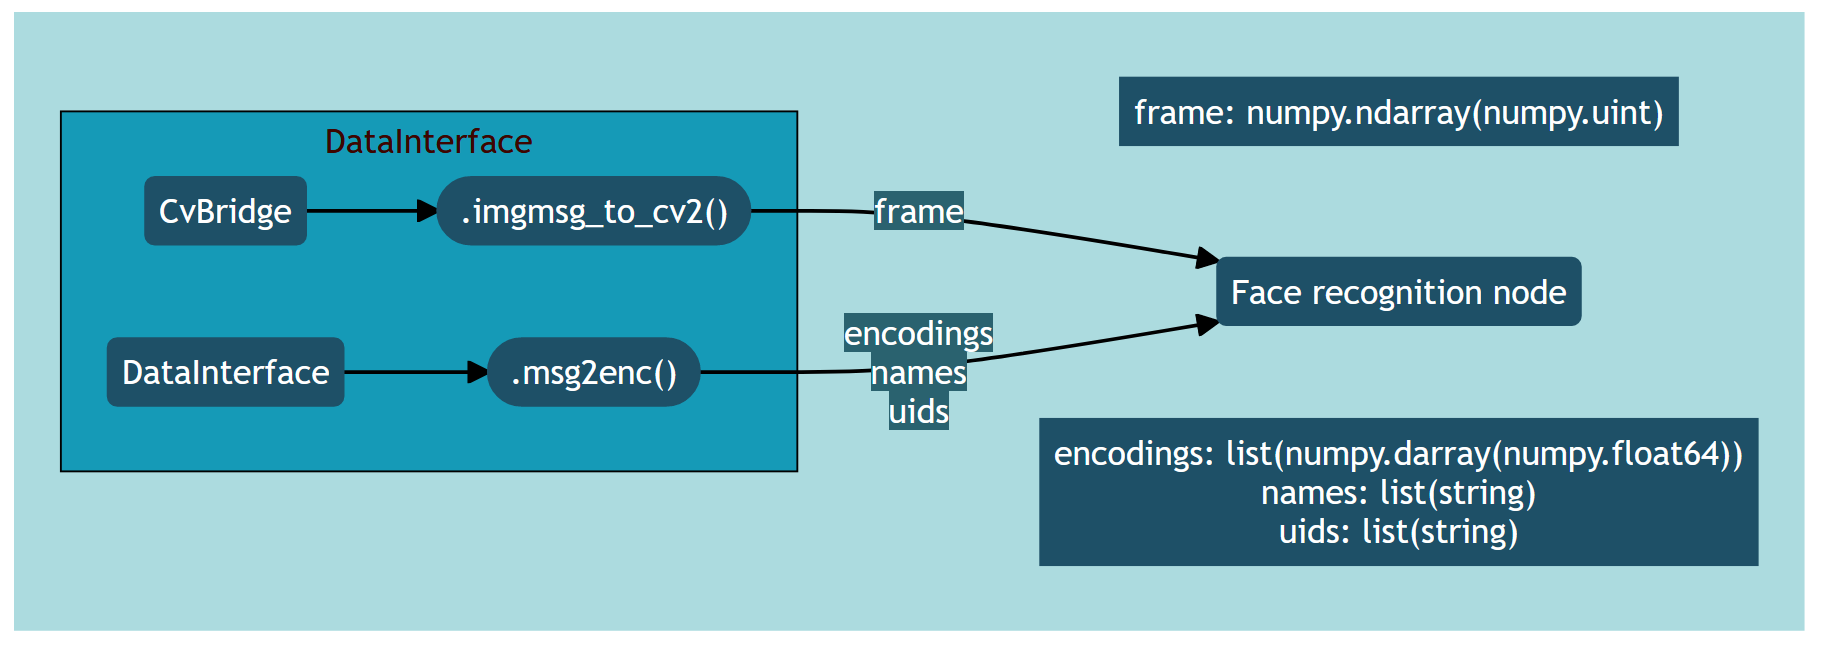
\includegraphics[width=151mm, keepaspectratio]{02_mermaid/fr_bemenet2.png}
    \caption{Arcfelismerést végző „node" bemenetei.}
    \label{fig:fri}
\end{figure}

\subsubsection{Kimenetek}
A „node" kettő „publisher"-rel rendelkezik (\refstruc{fig:fro}), amelyből az első szolgál az arcokat megjelenítő kép továbbításáért. A második „publisher" a felismert emberek arcának adatait adja át az adatbázist kezelő „node" részére. Egy „service"-t ér el kliensként, amin keresztül lekérheti a szükséges adatbázist. 
\begin{figure}[!ht]
    \centering
    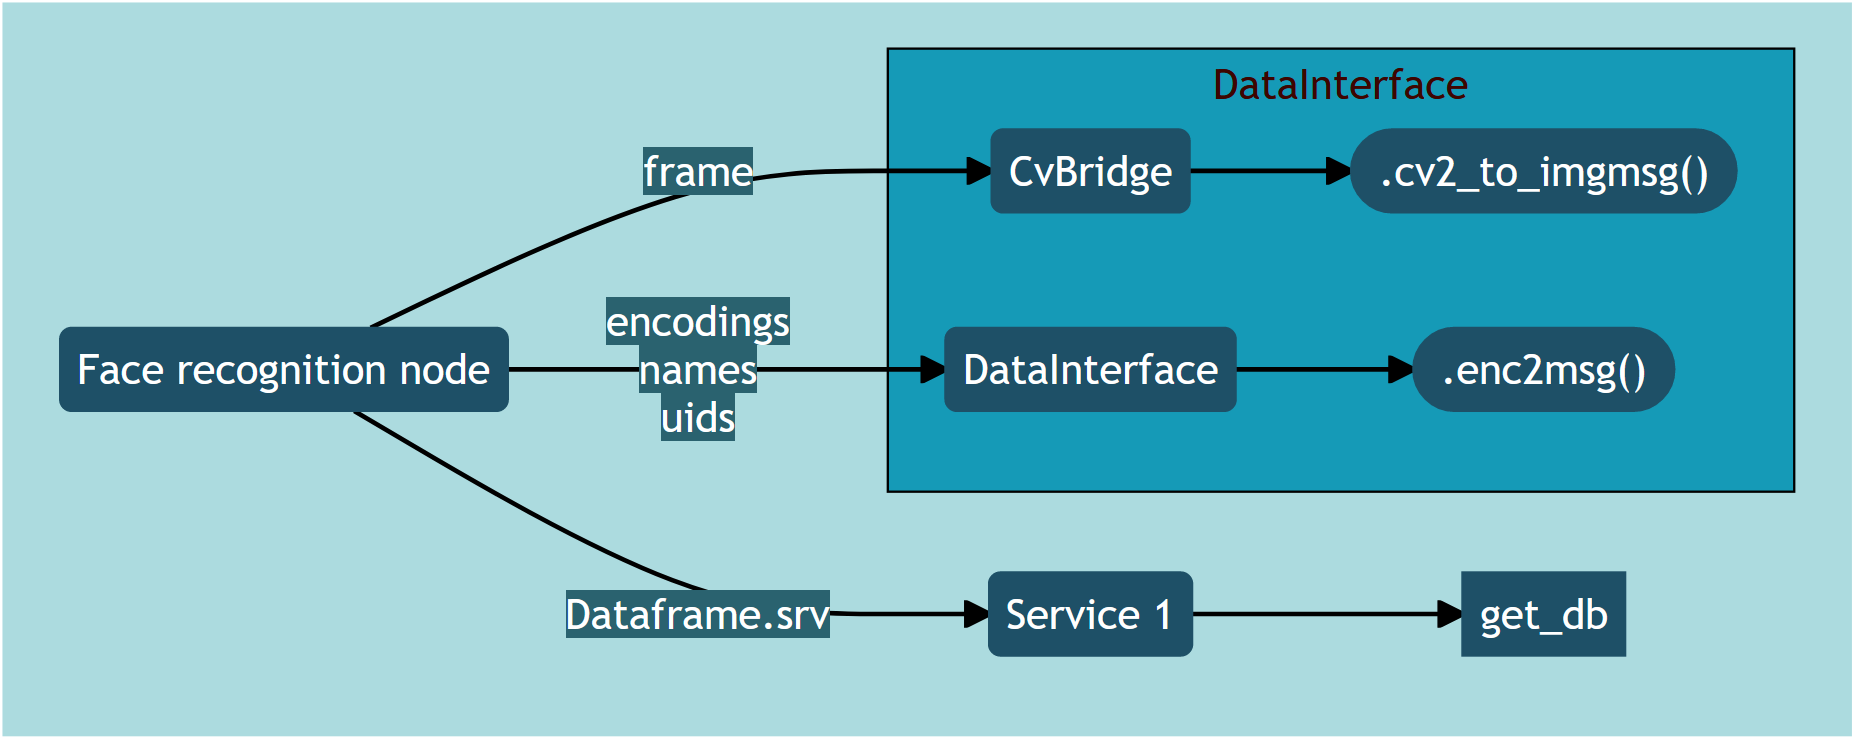
\includegraphics[width=150mm, keepaspectratio]{02_mermaid/fr_kimenet1.png}
    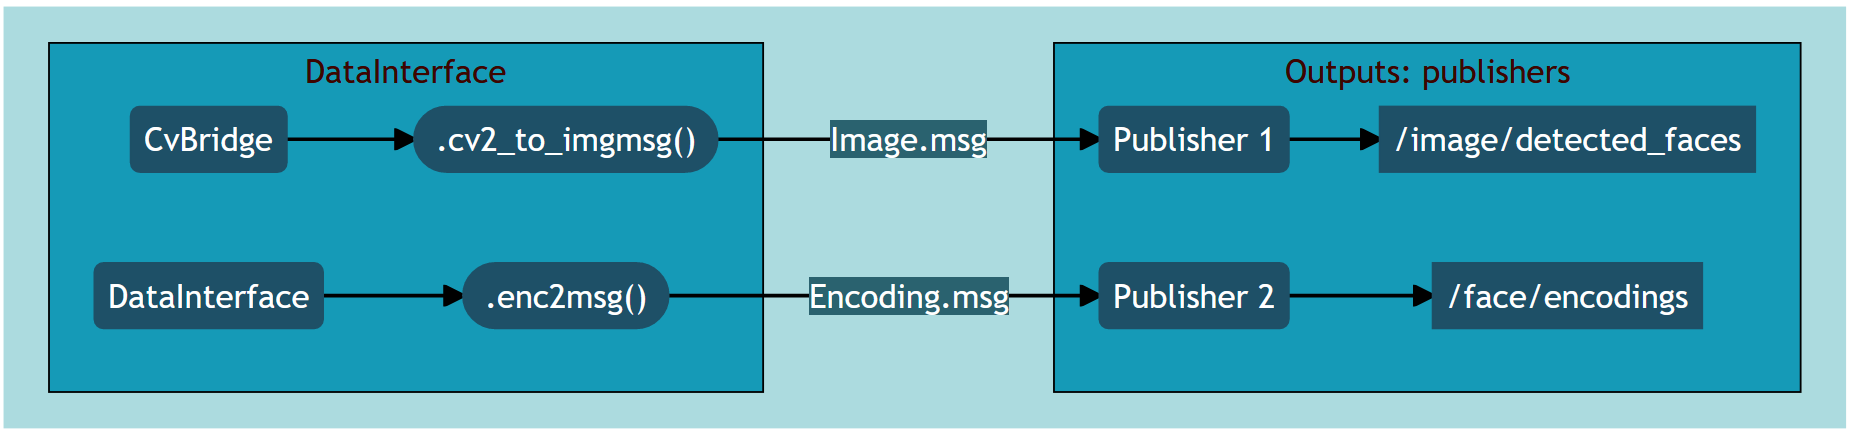
\includegraphics[width=150mm, keepaspectratio]{02_mermaid/fr_kimenet2.png}
    \caption{Arcfelismerést végző „node" kimenetei.}
    \label{fig:fro}
\end{figure}

\subsubsection{Részletes működés}
%todo mellékletben ábrát berakni initről
A „node” inicializálásakor példányosítja az \verb|ImageProcessor|-t és a \verb|DataInterface|-t. Az \verb|src/image_processor.py| fájlban van az \verb|ImageProcessor| osztály, amit a képkockák feldolgozására írtam. A \verb|DataInterface| osztályt a \verb|src/data_interface.py| fájlban implementáltam a gyakran előforduló adattípusok közötti konverzió lekezelésére. Ezeket közös „namespace”-be fordítom, így a csomag össszes „node”-jából elérhetőek. Ezekről részletesebben a következő fejezetben írok. Szintén az \verb|inti(self)| függvényben beállítom az arcok észlelésénél szükséges tolerancia értékét 0.6-nak választottam. Itt fut le egy kérés az adatbázist biztosító „node” felé, amiben lekérem az indításhoz szükséges adatbázist. Az adatbázis kialakítást részletesen az adatbázis „node” fejezetében fogom tárgyalni. Az arcfelismerést végző „node” működésének megértéséhez a lényeg, hogy létezik egy kisméretű adatbázis az adatbázist kezelő „node”-on belül, melyben megadható azon emberek arcainak enkódolása, akikkel potenciálisan gyakran találkozik a robot. Ezt az adatbázist egy „request”-en keresztül kéri le, és tölti fel a benne található adatokkal a „cache”-t. Ennek gyakorlati célja, hogy a mindenkori bemenetként szolgáló képen észlelt arcokat először ebben a „cache”-ben található arcokkal veti össze így gyorsítva a feldolgozást. A fel nem ismert arcokat a \verb|/face/encodings| „topic”-on adja át az adatbázisnak, ami elvégzi ezeknek a feldolgozását szimultán. Egyszerre fut a két „node”, így az adatbázis „node”-ban a megkapott ismeretlen arcok szortírozása nem akadályozza a kamera képének valós idejű feldolgozását.

Inicializáláskor regisztrálom a „publisher”-eket és egy „subscriber”-t, továbbá a szükséges lokális változókat.  
Az \verb|/image/webcam/raw| „topic”-ra feliratkozva éri el a webkamera képét. Minden „topic”-on megjelenő üzenet után meghívja a „callback” függvényét (\refstruc{fig:fcb}), amiben először „cv\textunderscore bridge" segítségével visszaalakítja az üzenetet egy olyan adattípusra amin már el tudja végezni a feldolgozással járó műveleteket. 

\begin{figure}[!ht]
    \centering
    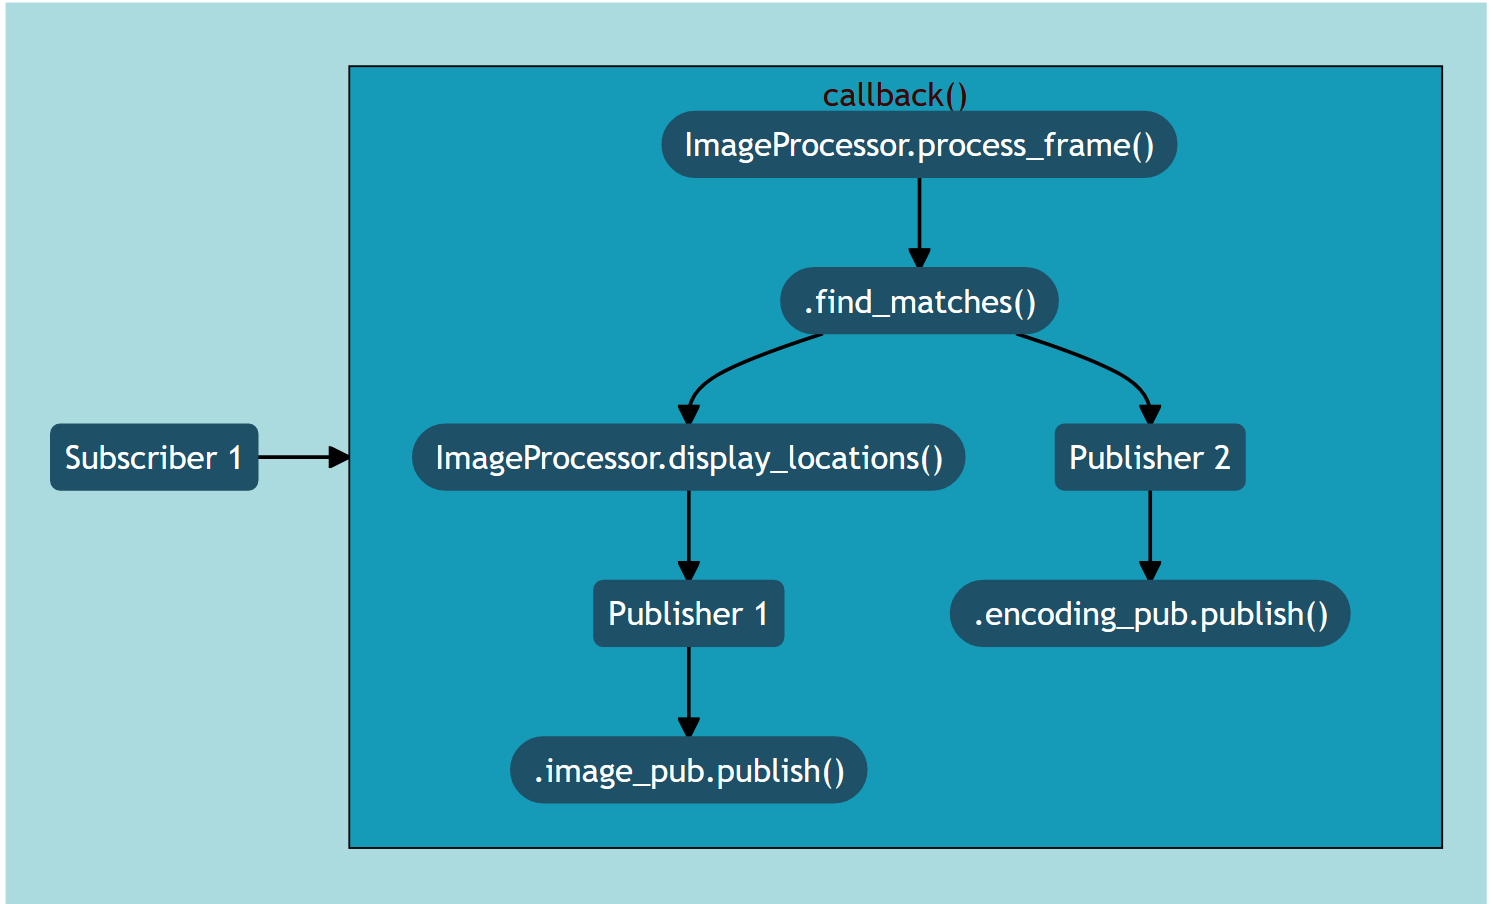
\includegraphics[width=125mm, keepaspectratio]{02_mermaid/face_callback.png}
    \caption{Arcfelismerést végző „node" „callback" függvényének működése.}
    \label{fig:fcb}
\end{figure}

Az üzenet átalakítása után a kapott képkockán először az \verb|ImageProcessor| osztály segítségével \verb|.process_frame()| függvénnyel elvégez egy arc keresést, amely visszaadja az adott képkockán található emberi arcok helyét és enkódolását. Ezt minden másik képkockán végzi el, csökkentve a hardver terhelését. A rendszer működésének tekintetében, mivel másodpercenként 25 képkockát rögzítünk (tesztelés során) ezért van bőven elég adatunk arról, hogy kiket lát a robot, szóval a teljes folyamat szempontjából jelentéktelen, hogy minden második képkockát kihagyunk. Az arcok lokációja és enkódolása egy-egy lista, amely elemszáma a képen észlelt emberi arcok száma. A helyszín lista elemei is listák. Egy arc helyét egy köré rajzolható téglalappal lehet legegyszerűbben definiálni, amit négy „integer” számmal határozza meg a „face-recognition” modul: kettő koordinátával, amik egy csúcsot jelölnek (bal felső csúcspont) és a téglalap két oldalának hosszával. Az enkódolás szintén két dimenzióban értelmezhető, az egyik dimenzió az észlelt arcok száma, a másik 128 darab „float64” típusú számból álló lista. Ezek a 128 elemű listák írják le az egyénre jellemző vonásokat. Hogy ezen belül melyik szám mit jelent, arról nincs információnk, mert ezeket egy konvolúciós háló állítja elő, aminek a belső működése számunkra egy fekete-doboz. Ugyanakkor ez a működés jelen esetben nem is jelentene semmilyen plusz információt, csupán azt az egy dolgot kell tudnunk, hogy két 128 elemű lista annál jobban fog egymáshoz közelíteni, minél jobban hasonlítanak az arcok. Ha két különböző képen ugyanazt az embert látja, akkor közel ugyanazt a 128 elemű listát kapjuk vissza. Ezen alapul az arcok összehasonlítása.

Az arcok lokációinak és „enkódolásainak” birtokában még az eredeti „callback”-en belül elvégez egy arcfelismerést. Az összes észlelt arcot összehasonlítja az összes „cache”-ből betöltött arccal. Ezt az összehasonlítást a \verb|find_matches()| függvény végzi. Végig iterál a „cache”-ben tárolt arcokon és mindegyikkel összeveti az észlelt arcokat a \verb|face_recognition.compare_faces()| függvénnyel. A ciklus annyiszor fut le ahány arcot talált a program a képen. Minden ciklusban a fenti függvény kimenete egy „boolean” lista. A tárolt arcok sorrendjének megfelelően igazat vagy hamist ad annak függvényében, hogy a beállított tolerancia érték szerint hasonló arcot talált-e. Szintén ugyanebben a ciklusban, amiben az észlelt arcok listájából egyet vet össze az összes eddig eltárolt arc információjával, megvizsgálja milyen távolságra van tőlük \verb|face_recognition.face_distance()| függvényben. A távolságot euklideszi térben kell értelmezni. Már említett módon, a konvolúciós háló ad bármely arcról egy 128 elemű listát. Gyakorlatilag egy 128 dimenziós térben számolja a függvény a távolságot. Az arcok összehasonlításának egy lista lesz az eredménye, mely tartalmazza rendre a tárolt arcoktól való távolságát, ami azt reprezentálja mennyire hasonlít hozzájuk. Ezt a listát összevetve azzal, amiben azt tároljuk, hogy melyik arc reprezentál találatot, a találatok közül ki tudjuk választani azt, aminek a legkisebb a távolsága a vizsgált arctól.

A \verb|find_matches()| függvény az észlelt arcokat kettőféleképpen csoportosítja: felismert, ezeket ellátja az adatbázisból kiolvasott névvel, illetve nem felismert „Unknown”, az olyan arcok akikkel nem talált egyezést a betöltött „cache”-ben. A függvény kimenete két lista: nevek és „uid"-k, mindkettő az észlelt arcok „enkódolásait” tartalmazó lista sorrendjének felel meg. A név lista értelemszerűen az „enkódoláshoz" tartozó név változókat tárolja „string” formátumban. A „uid” listában, szintén „string” adattípusban annak az arcnak az egyedi azonosítóját tartalmazza, amihez a vizsgált „enkódolás" legközelebbi egyezést talált. Ez pedig arra szolgál, hogy miután a „node” átadja az adatbázis-t kezelő „node”-nak a listákat a feldolgozás során tudja növelni egyel az értékét a megfelelő archoz tartozó találat számláló mezőnek.

A \verb|find_matches()| függvény visszatérési értéke egy „boolean” változó, a függvény elején vizsgálom, hogy a helyszíneket tartalmazó lista hosszabb-e, mint nulla azaz, talált-e arcot. Ha nem akkor nem is végzi el az összehasonlításokat és hamis értékkel tér vissza. Ha hosszabb a lista, mint nulla, tehát az előző \verb|ImageProcessor.process_image()| függvény észlelt emberi arcot, akkor elvégzi az összehasonlítást és felülírja az osztályváltozóként deklarált nevekből és „uid”-kból álló listákat. Ezt a visszatérési értéket vizsgálom a következő lépésben. Az arcokat a képkocára rajzoló függvény az \verb|ImageProcessor.display_faces()| csak akkor fut le, ha észlelt arcokat a program. Ennek a kivitelezésnek az oka a spórolás az erőforrásokkal. Egyértelmű, hogy ha nem észleltünk arcokat nincs szükség azok kirajzolására, tehát felesleges meghívni a \verb|.display_faces()| függvényt. Abban az esetben, ha észleltünk arcokat és meghatároztuk a nevüket, legyen ismert név vagy nem ismert „Unknown”, kirajzoljuk a „locations” listában található koordináták alapján az arcokat jelölő téglalapot és aláírjuk a hozzátartozó nevet. Háromféle kategóriát különítek el a kirajzolásnál. Az első a névvel felismert arcokat  zöld színnel, a felismert, de név nélküli „Unknown\textunderscore id” arcokat kékkel és a még nem osztályozott „Unknown” arcokat pirossal rajzolja ki a függvény. A képkockára rárajzolás után a módosított képkockát publikálom az \verb|/image/detected_faces| „topic”-on. A „topic”-ra való közlést megelőzi egy átalakítás a \verb|CvBridge.cv2_to_imgmsg()| segítségével. Gyakorlatilag a kép üzenet formátumot fogadó „callback” függvény egy üzenet adattípusban kapja meg a képet, amit vissza alakít cv2-ben és „face-recognition"-ben feldolgozható képpé, majd a feldolgozást követően visszaalakítja üzenet formátumba, hogy ROS keretrendszerben elküldhető legyen.

Ezt a publikálást minden „callback” híváskor végrehajtom, hogy a kimeneti kép folyamatos legyen. Ugyanakkor beépítettem, már fentebb kifejtett módokon, az erőforrásokkal való spórolás céljából különböző ellenőrző lépéseket, tehát nem minden „callback” híváskor módosul az üzenetként megkapott kép. Ha nem talál arcot, akkor ugyanazt a megkapott képet továbbítja, csak egy különböző „topic”-ra. A kép publikálása után, ami minden hívásban megtörténik, implementáltam még egy publikálást, amiben nem képet, hanem az azon észlelt majd felismert arcokhoz tartozó információkat („enkódolás", név, „uid”) listákat küldöm a \verb|/face/queried_encodings| „topic”-ra. Ez az adatbázis kezelő „node” számára való információ átadás csatornája. Itt két erőforrás felhasználást csökkentő lépést iktattam be. Egyrészt vizsgálom, hogy talált-e emberi arcot a képen, ha nem akkor felesleges elküldeni a nulla elemeket tartalamazó listákat. Másrészről egy időzítő osztályváltozót hoztam létre, ami 25 „callback” hívásonként engedélyezi csak a közlést a „topic”-on. Erre azért van szükség, mert az adatbázist kezelő „node” erre a „topic”-ra feliratkozott „callback” függvényének a futásideje hosszú és műveletigényes. Ha emberi viselkedéshez akarjuk hasonlítani, itt történik meg az, amikor meglátunk egy arcot, nem jut eszünkbe a személy neve, és elkezdünk rajta gondolkozni. Nincs szükségünk arra, hogy másodpercenként 25 képet alkossunk arról az arcról, elég egyszer „ránéznünk" (mintavételeznünk). Így implementáltam a programban is. Ha 25 képenként, azaz 1 másodpercenként (mivel 25 fps-el rögzít) látunk egy emberi arcot, akkor már elkészíti róla az „enkódolást", amit átadhat az adatbázisnak a bővebb felismerés lefolytatásához. De erről a folyamatról részletesebben az adatbázis kezelő „node” leírásában írok.

\subsection{Arcok észlelését végző osztály}

Ebbe az általam írt osztályba szerveztem ki az arcok felismerését és képkockára rajzolását. A csomag kimenete az élő webkamera kép, rajta az arcok helyét jelölő kerettel és a keret alatt egy négyzetben az emberek nevével.
Osztályváltozóként lehet megadni a színkódokat; három különböző színnel ad visszajelzést, ami az emberek felismertségét jelenti. Zöld színnel az inicializáláskor megtanított emberek arcát jelöli, akikhez név is társul, kékkel az egyszer már látott és elmentett arcokat, ahol a név: „Unknown\textunderscore id” és a még nem elmentett, először látott arcokat pirossal és „Unknown” névvel.

Az osztály két fügvénnyel rendelkezik, az első: a \verb|.process_frame(frame)|, ahol a \verb|frame| változóban megadott képkockán végzi el az arcok keresését. Először a megadott \verb|factor| értékkel méretezi át a képet. Ez a lépés erőforrás optimalizálás céljából indokolt. Kisebb kép is tartalmazza ugyanazt az információt az arcokról, ami szükséges a sikeres felismeréshez, de kisebb méretű képet hamarabb dolgoz fel az algoritmus, kevesebb erőforrás igény mellett.  Ez után a képet át kell alakítani RGB formátumra. A cv2 modul által rögzített képkocka egy több dimenziós mátrix, ahol minden pixelnek van három szín értéke, melyeket nem piros-zöld-kék sorrendben tárol, hanem kék-zöld-piros sorrendben, mely a modul sajátossága. Viszont a „face-recognition” modul számára RGB formátumú képre van szükség. Az áttranszformálás után ez az első függvény megkeresi az arcok helyét, amit egy egy dimenziós listaként kapunk meg, majd a helyek segítségével megalkotja az arcokhoz tartozó enkódolást. Ez egy „n” dimenziós lista, ahol „n” az arcok száma és mindegyik eleme egy 128 elem hosszúságú lista, ami az arcok reprezentációjára szolgáló vektor értékeit tárolja. A függvény kimenete a helyszín lista és az enkódolások listája.

A második függvénye az osztálynak a \verb|.display_locations()|. A függvény argumentumai: \verb|frame| – a képkocka amire rajzol, \verb|locations| – az arcok helyei a képen, és a \verb|names| – az arcok nevei. Mivel az arcok koordinátáit méretezett képen határoztuk meg, ezért át kell őket transzformálni, ez egy szorzást jelent a \verb|.process_frame()|-ben használt tényező reciprokával. A kapott koordinátákkal a cv2 modul \verb|.rectangle()| és \verb|.text()| függvényeivel a képkockára rajzolja az arcok köré a keretet a megfelelő színnel és alá írja a neveket. A függvény a módosított képkockával tér vissza. Paraméterek, amiket tetszés szerint meg lehet választani: betűtípus, betűméret, színek, keret vastagsága.

\subsection{Adatbázis}
Az adatbázis 6 oszlopból épül fel (\refstruc{tab:adatb}) és minden arcról készített enkódolás külön sort képez. „Name” oszlopban a személy neve, arcának „enkódolása” pedig a „Face” oszlopban van. Minden archoz tartozik egy egyedi „uid” (az „Id" oszlopban), ennek az azonosítás és az adatok megkülönböztetésének szempontjából van szerepe. A „Folder” és „Filename” oszlopok azon „enkódolásokhoz" tartozó fájlok és mappájuk nevét jegyzik, amik a csomag \verb|images| mappájában találhatók. Az új látott arcok feldolgozása során az adatbázis korábbi adataival hasonlítja össze őket, és számolja, hogy melyiket találta optimális egyezésnek. Ezt az adatot a „Matchcounter” oszlop gyűjti, egy egész „integer” számmal jelöli hányszor bizonyult találatnak egy adott enkódolás az összehasonlítás folyamán. Ahányszor pozitív egyezést talál megnöveli egy számmal. Innen lehet következtetni arra, hogy mely enkódolás a legpontosabb egy arcról.
\begin{table}[!ht]
	\footnotesize
	\centering
	\begin{tabular}{ l c c }
		\toprule
		Elnevezés & Jelentés & Típus \\
		\midrule
        Name & archoz tartozó név & string\\
        Id & uid & string\\
        Folder & mappa neve & string\\
        Filename & fájl neve & string\\
        MatchCounter & egyezések száma & integer\\
        Face & enkódolás & list\\
		\bottomrule
	\end{tabular}
	\caption{Az adatbázis oszlopai.}
	\label{tab:adatb}
\end{table}

Mivel az adatbázis minden elemét meg kell különböztetnünk egymástól, ezért kell egy attribútum, ami alapján ezt elvégezhetjük. A név nem egy jó választás, mivel egy ember arcáról több „enkódolást" is le tudunk menteni. Mappa és fájlnév sem használható, mert ezzel csak az adatbázis inicializálásakor betöltött enkódolások rendelkeznek. Ezért hoztam létre egy külön „Id” oszlopot amiben a Python egy moduljának \verb|uuid.uuid4()|\footnote{python uuid: \url{https://docs.python.org/3/library/uuid.html}} függvényével generálok egy véletlenszerű azonosítót RCF4122 szabvány\footnote{RCF4122 szabvány: \url{https://www.rfc-editor.org/rfc/rfc4122}} szerint. Ezt utána „string”-ként tárolom, mivel ilyen formában át tudom adni „message”-eken és „service”-eken keresztül. Mivel ROS-on belül nincs „uuid” osztály, ezért csak „string”-re átalakítva tudom „node”-ok között átvinni. Logikátlan lett volna, ha nem „string”-ként tárolom, mivel rendszeresen oda és vissza kellett volna alakítanom. Így egyszer létrehozáskor átkonvertálom „string”-é és utána bármikor használható és összehasonlítható lesz.



%TODO: „uid” – stringben tárolás könnyű összehasonlítás python példa jupyter notebook
%TODO2: táblázat az adatoknak
%Name (név): string
%Id (egyedi azonosító): string
%Folder (mappa): string
%Filename (fájlnév): string
%MatchCounter (találatok száma): int
%Face (arc kódja): tömb valami…

\subsection{Adatbázist kezelő node}
A \verb|face_database.py| fájlban található \verb|FaceDatabase| „node" feladata, hogy adatbázist biztosítson az arcokról készített enkódolások tárolására. Adatbázis gyanánt a Pandas modul \verb|DataFrame| osztályát használom, amit a könnyű kezelhetősége és kis tárhely igénye miatt választottam. További előnyei, hogy nincs szükség külön adatbázis például MySQL futtatására. Mindezek mellett fontos tervezési lépésként úgy döntöttem, hogy készítek egy \verb|DatabaseManager| osztályt, ami abban a tekintetben bonyolít a csomag felépítésén, hogy egy plusz architekturális réteg került bevezetésre. Előnye, hogy ebben az osztályban a Pandas féle \verb|DataFrame| specifikus lekérdezések és adatmódosítások kicserélhetőek másik adatbázis kezelő moduléra. S mivel az adatbázist kezelő „node”-ban nincsenek közvetve meghívva a \verb|DataFrame| osztály tagfüggvényei, a saját \verb|DatabaseManager| osztály függvényeit használja. Ennek a tervezési döntésnek köszönhetően nem jelentene semmilyen problémát, ha másik adatbázis kezelőre cseréljük ki. 

A „node” a ROS-on belüli kommunikációhoz egy „subscriber”-t, egy „publisher”-t használ (\refstruc{fig:dbio}). A \verb|/face/encodings| „topic”-ra feliratkozott „subscriber”-rel kapja meg az élő kamera képén észlelt, felismert emberek arcainak enkódolását, neveit, „uid”-ját. A \verb|/face/queried_encodings| „topic”-on publikálja a lekért emberekhez tartozó arcok neveit. Egy „service” biztosítja az indításkor a „face-recognition” „node” felé a kezdő adatbázis lekérését.

\begin{figure}[!ht]
    \centering
    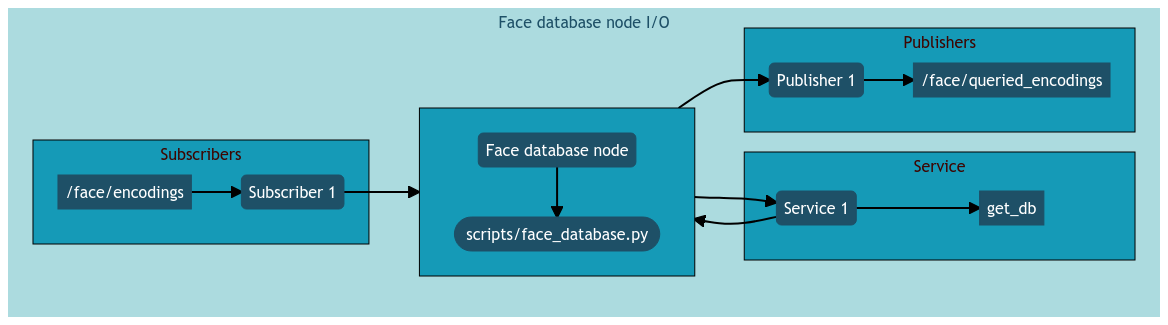
\includegraphics[width=150mm, keepaspectratio]{02_mermaid/mermaid30_db_io.png}
    \caption{Adatbázist kezelő „node" „I/O"-ja.}
    \label{fig:dbio}
\end{figure}

\subsubsection{Bemenetek}
Az adatbázis kezelő „node” a bevett szerver-kliens architekturális elrendezésben szerverként viselkedik, mellyel lekérhető futásidőben az adatbázis. Jelenleg a működés szempontjából lényeges kezdő adatbázis lekérésre van lehetőség. A \verb|get_db| név alatt kínál egy meghívható „service”-t amit bármelyik „node”-ból le lehet kérni, ez a funkcionalitás is a ROS alapelveinek köszönhető. A csomag robotra illesztésekor ennek köszönhetően más csomagok „node”-jaiból indított „request”-el el lehet kérni az adatbázist, ha erre szükség lenne. A csomagomban jelenleg egy „node”-ban implementáltam a hívást. A „face-recognition” „node” küldhet „request”-et az adatbázis kezelő „node”-nak amellyel inicializáláskor áttölti a kezdő adatbázis tartalmát a saját „cache”-be.

A \verb|/face/encodings| „topic”-ra feliratkozott „subscriber” felelős azért, hogy az arcokat felismerő „node”-ban erre a „topic”-ra küldött adatokat beolvassa. Minden publikált adatcsomagnál meghívja a „callback” függvényt, ami feldolgozza ezeket. Mivel ROS-on belül nincs lehetőség több dimenziós lista vagy tömb elküldésére, ezért egy dimenziós formában érkeznek az adatok, amiket a \verb|DataInterface| osztály \verb|.msg2enc()| függvényével alakítja vissza a megfelelő formátumra.

\begin{figure}[!ht]
    \centering
    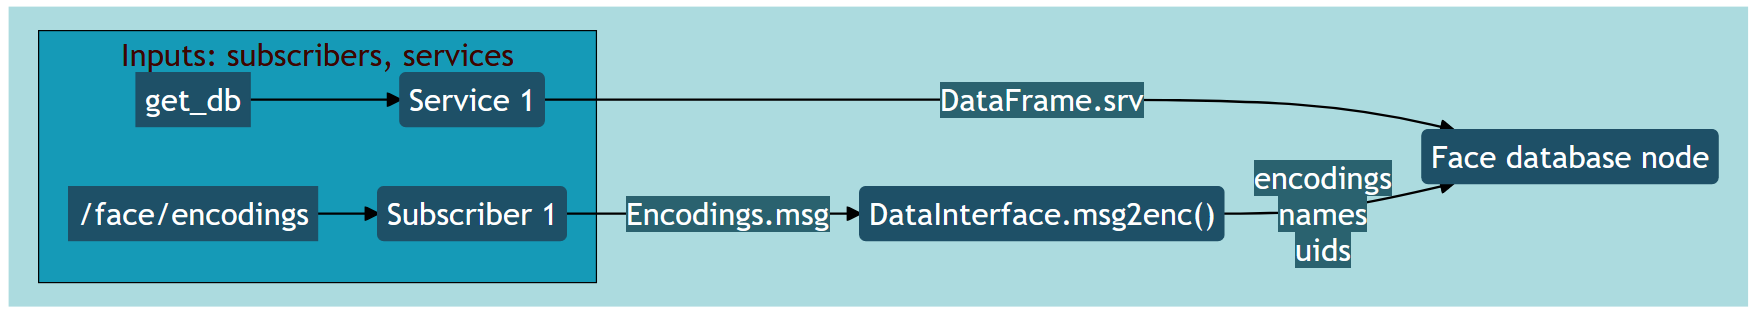
\includegraphics[width=150mm, keepaspectratio]{02_mermaid/db_bemenet1.png}
    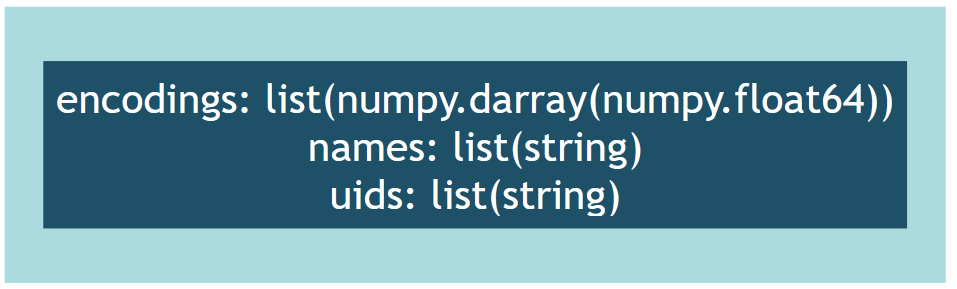
\includegraphics[width=70mm, keepaspectratio]{02_mermaid/db_bemenet2.png}
    \caption{Adatbázist kezelő „node" bemenetei.}
    \label{fig:bdi}
\end{figure}

\subsubsection{Kimenetek}
A \verb|get_db| „service” az előző fejezetben leírtak szerinti meghívásakor küldi el a szükséges adatokat. Emellett a „publisher” biztosítja a lekért arcokhoz tartozó adatok publikálását az arcfelismerést végző „node” felé. Itt szintén a \verb|DataInterface| osztály felhasználásával fordul le az adatbázis struktúrájának megfelelő tartalom.
\begin{figure}[!ht]
    \centering
    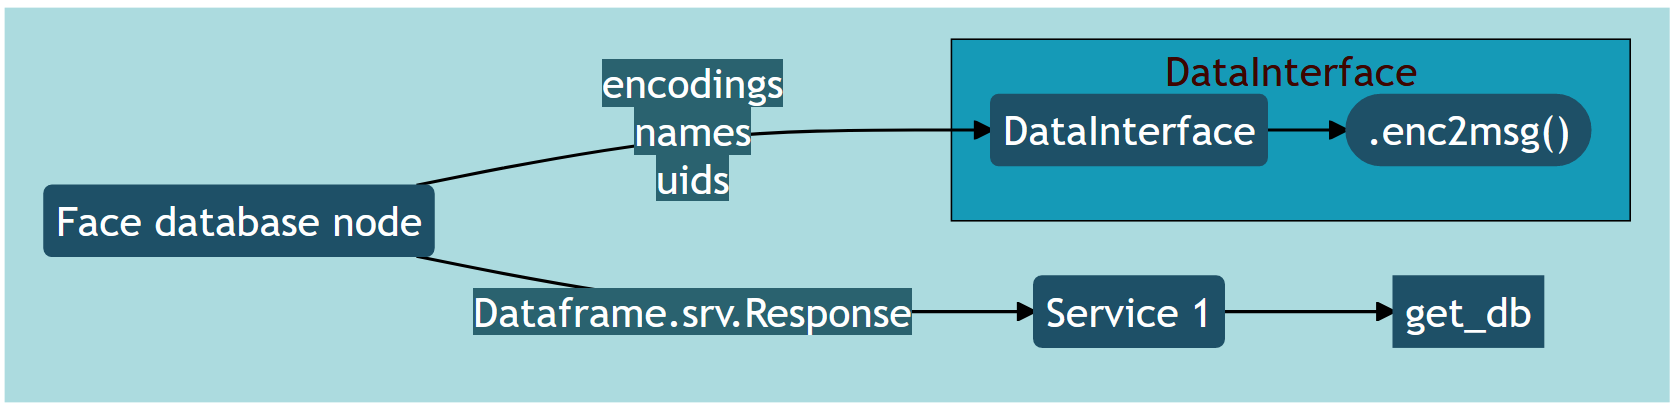
\includegraphics[width=150mm, keepaspectratio]{02_mermaid/db_kimenet1.png}
    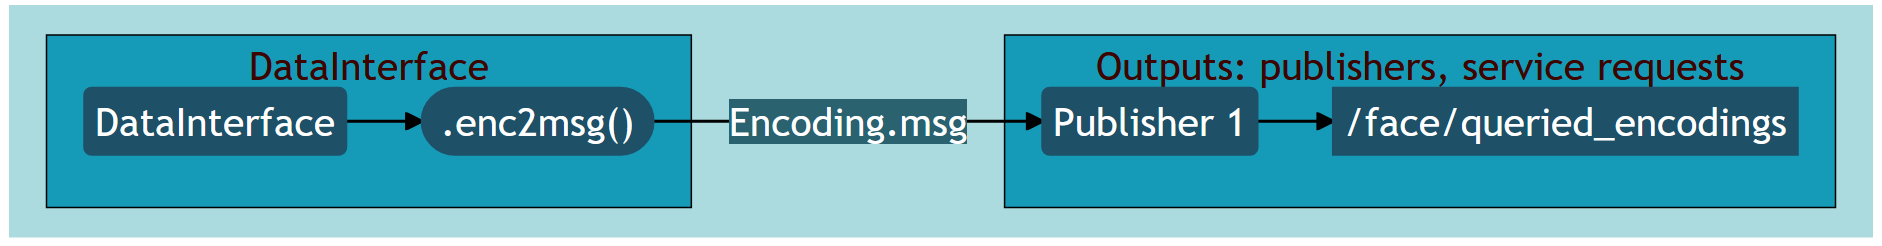
\includegraphics[width=150mm, keepaspectratio]{02_mermaid/db_kimenet2.png}
    \caption{Adatbázist kezelő „node" kimenetei.}
    \label{fig:dbo}
\end{figure}

\subsubsection{Részletes működés}
A \verb|face_database.py| \verb|main| függvénye a szokványos felépítést követve először inicializálja a „node”-ot, majd a megadott „rate” frekvencia értékkel futtatja \verb|rospy.spin()| fügvénnyel. A „FaceDatabase” osztály a „node” implementációjának kezdésekor beállítja az osztály változóit, inicializálja a „subscriber”-t és „publisher”-t. Valamint létrehozza az adatbázisokat. Leállításakor elmenti a használt adatbázist.

A függvény három adatbázist hoz létre. Az első „Start” vagy kezdő adatbázis, ezzel töltődik fel a „face-recognition”-ben a „cache”. Ez az az adatbázis, amely azon a kulcsfontosságú emberek adatait tartalmazza, akiket előreláthatólag gyakran kell felismernie a robotnak. Az arcfelismerést végző „node” először ebben az adatbázisban kutat egyezés után, ha nem talál, akkor adja át az adatbázist kezelő „node”-nak az észlelt arcok „enkódolását”. A második és harmadik adatbázis megegyezik tartalom tekintetében inicializáláskor. Mint az a kódban is látható, a „Main” vagy fő adatbázist fájlból olvassa ki és utána a futásidőben használt „live\textunderscore df” vagy élő adatbázis adatait innen másolja ki. A programkód futás közben ezt a „live\textunderscore df” adatbázist módosíthatja csak, a fő adatbázist nem tudja szerkeszteni. Azért ezt a megoldást használom, mert előnyös, hogy ha van egy olyan adathalmaz, amihez bármilyen meghibásodás, vagy zavar esetén vissza tudunk térni. Ennek a funkciónak az implementálására azért volt szükség, mert a \verb|pandas.DataFrame| osztály nem rendelkezik beépített biztonsági mentés kezelő funkcióval. Az adatbázisok kezelésére írt \verb|DatabaseManager| osztály inicializálja az adatbázisokat. Ha nem találja a fájlokat, akkor létrehozza és feltölti őket a rendelkezésre álló adatokkal. Ezeket az adatokat képekből nyeri ki, amelyeket megadhatunk a csomag \verb|/images/known_faces/| mappájában. A struktúra, amit felépítettem az arcok tárolására az alábbi: minden ismertnek titulált arcról készült képet az előző mappában személyenként külön-külön mappába kell rendezni. Lehetőség szerint a képen egy ember legyen látható, mert az algoritmus jelen implementációja szerint egy fájlt csak egy archoz tud társítani, ha több ember szerepel a képen akkor az először észlelt arcot kapcsolja a névhez. A személy nevét a mappa neve adja. Tehát, például ha \verb|/images/known_faces/mate| mappában talál a szoftver három \verb|.png| kiterjesztésű fájlt, akkor beolvassa mindegyiket, és hozzájuk a mappa nevét, azaz „mate” nevet rendeli. Az emberek elnevezése innen származik, ezt későbbieknek (a képek beolvasása után) nem lehet megváltoztatni viszont az utólagos név választás vagy módosítás funkcióját könnyen lehet implementál, egy „service” segítségével. Ez az adatbázisban egy megadott „uid”-hoz tartozó sor nevet tartalmazó mezőjét átírja a „request”-ben „string” típusban megadott értékre.

A \verb|/face/encodings| „topic”-ra feliratkozott „subscriber” meghívja az osztály „callback” függvényét (\refstruc{fig:dbcb}). Ebben a fügvényben történik az adatok feldolgozása. A megkapott adatokat a \verb|DataInterface| osztály segítségével átalakítja a  „node”, mellyel megkapja az élő kamera képről felismert emberi arcokat. Az arcokat kétféleképpen osztályozza a „face\textunderscore recognition\textunderscore core.py”-ban futó „node”.
\begin{figure}[!ht]
    \centering
    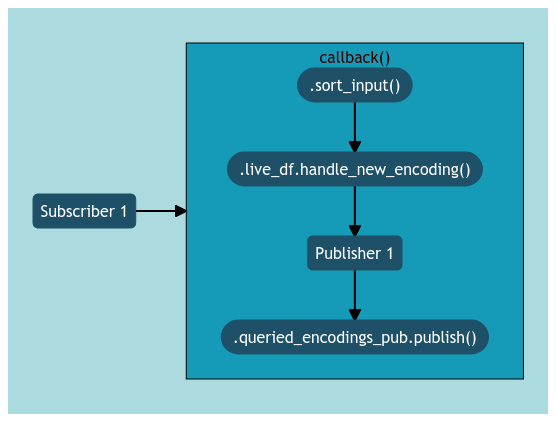
\includegraphics[width=100mm, keepaspectratio]{02_mermaid/mermaid34_db_callback.png}
    \caption{Adatbázist kezelő „node" callback függvénye}
    \label{fig:dbcb}
\end{figure}

Ha talál a „cache”-ben egyezést a felismert arcokhoz, amiket az enkódolás képvisel, akkor hozzá társítja a létező találatot jelentő ember nevét és a találat „uid”-ját. Ennek a „uid”-nak abban van szerepe, hogy a „callback” függvény így megtalálja az adatbázisból az egyezést biztosító elemet és megnövelje a „MatchCounter” mező számát. Innen lehet következtetni, hogy egy elem hányszor biztosított megfelelő felismerést. Minél közelebbi a két enkódolás, annál pontosabb az egyezés. Tehát megállapítható a „MatchCounter” száma alapján: minél nagyobb annál jobb alapot biztosított bizonyos ember felismeréséhez. Ezt követően a művelet generál egy új egyedi „uid”-t amit hozzá társít ehhez a beérkező „enkódolás”, név pároshoz és elmenti az adatbázisba. 


Ha nem talált a „cache”-ben egyezést, akkor „Unknown”-ként jelöli meg. Ez két opciót jelenthet. Az első, hogy van információnk az illetőről, de még azt nem töltöttük át a „cache”-be. A második opció, hogy valóban ismeretlen ember állt a kamera előtt. Emiatt szükséges egy összevetést végeznünk a teljes adatbázison, hogy kiderüljön létezik-e a látott ember arcához tartozó enkódolás.
Ez volt a fő tervezési gondolat a „cache” létrehozása körül. Tulajdonképpen megrövidítem azoknak az elemeknek a számát, amin végig kell iterálnia, így biztosítva az arcfelismerésre szolgáló „node” kimenetének késésének minimalizálását. Ha csak egy kisebb méretű „cache”-t kell ellenőriznie gyorsabban végez vele, mint ha az egész adatbázison tenné ugyanezt. A fel nem ismert enkódolások átadásával átszerveztem a sok feldolgozást követelő, időigényes műveletet az adatbázis kezelő „node”-ba. Itt párhuzamosan futhat és ha végzett visszatérhet aszinkron a \verb|/face/queried_encodings| „topic”-on a keresett elemekkel. Így nem lassítja az arcfelismerő „node” működését, ami ennek köszönhetően folyamatosan tud adatot biztosítani az egész csomag kimenetének tekintendő \verb|/image/detected_faces| képfolyamon.

Az „Unknown” vagy névvel ellátott enkódolások beérkezése után lefolytatott feldolgozás során megállapítom, hogy valóban ismeretlen-e a személy, vagy már a robot egy előző alkalommal találkozott az emberrel. Ha találkozott, akkor az adatbázisból kiolvassa a kód az adatait és továbbítja a „cache”-be. Ha nem ismert, azaz valóban „Unknown”, akkor generál hozzá egy id-t, ami után elmentésre kerül „Unknown\textunderscore id” névvel, egy egyedi „uid”-val és a beérkezett enkódolással. Majd az elnevezést áttölti a „cache”-be. Mivel ez aszinkron módon párhuzamosan fut le az élő kamera képen végzett észleléssel, ezért nem kizárt, hogy a következő felismerési ciklus megkezdése előtt még nem éri el az arcfelismerést végző „node” „subscriber”-re, így újra lejátszódhat az egész folyamat. Itt lehetne a csomagot még optimalizálni, oly módon, hogy az adatbázist kezelő „node” lokálisan eltárolja a lekérdezett enkódolásokat és csak akkor végzi el az újak feldolgozását, ha ebben a lokális listában nincs jelen. Ennek a kivitelezésére nem találtam optimális megoldást, mivel az ugyanarról az arcról beérkező enkódolások is különböznek: mivel két kép nem egyezik meg tökéletesen, így nincs módom egy egyszerű összehasonlítást elvégezni, amivel meghatározhatom, hogy ezt az arcot vizsgáltam-e már. Pontosabban ugyanazt az összehasonlítást tudnám elvégezni a „face-recognition” modul függvényeivel, ami amúgy is lefut a beérkező „Unknown” arcok válogatásánál. Ezért nem láttam indokoltnak, hogy egy további lépéssel bonyolítsam és lassítsam a feldolgozást. Tervezői lépés, amit ezek ellenére megtettem, hogy minimalizáljam a duplán feldolgozást, hogy a \verb|/face/encodings| „topic” publikálást kisebb frekvencián végzem, nem minden képkocka vizsgálatánál, csak minden huszonötödiknél (25 képkocka per másodperc rögzítése esetén másodpercenként egyszer). Ez időt biztosít az adatbázist kezelő „node” „callback” függvények lefutására. Az adatbázis kezelésben ez nem okoz semmilyen hibát, kizárt, hogy kétszer legyen különböző „id"-val felvéve ugyanazon emberi arc, mert az adatbázis „node”-on belüli „callback” hívások egymás után futnak le időrendben. Tehát ha kétszer beérkezik egy valóban nem ismert arc, akkor első alkalomra társul hozzá egy „id" és rögtön bekerül az adatbázisba, így a második alkalommal történő futás közben már az adatbázisból húzza le az információkat.

Gyakorlati alkalmazásban ez úgy jelenik meg, hogy addig „Unknown” felirat van jelezve az arc alatt, amíg az osztályozás folyamata le nem futott. 

%TODO: leírni mennyi ideig jelenik meg lehetne grafikon - szép álmok
\subsection{Adatbázis menedzser osztály}
Architekturális elrendezésben a \verb|pandas.DataFrame| szintje fölé írtam egy osztályt, ami annak kezelhetőségét egyszerűsíti. Előnye, hogy egy példányban tartalmazza az adatbázis nevét, fájlnevét, elérési útvonalát a fájlrendszerben (amit, bárhol legyen a csomag le tud kérni az os\footnote{os.py: \url{https://docs.python.org/3/library/os.html}} modul segítségével), oszlopok neveit osztályváltozókban (tehát minden példány ugyanazokkal az adatokkal fog rendelkezni). Ennek az adatbázis menedzser osztálynak tagja a \verb|DataFrame| osztályból képzett saját változó, amiben az adatokat tárolom táblázatos formában. Egy új példány inicializálásakor az osztály felelős az adatok feltöltéséért. Itt implementáltam a fájlok beolvasását, az arcok betöltéséért felelős \verb|.load_known_faces()| függvényben. Megalkottam pár rövid függvényt, ami megkönnyíti a használatot. A \verb|.add_db(db)| függvénnyel, össze tudunk fűzni két \verb|DatabaseManager| osztályú változót. Amelyiken meghívjuk a függvényt, annak az adatbázisához adódik hozzá a paraméter. Az összefűzés után eltávolítja a duplán szereplő elemeket, az összehasonlítás alapját az egyedi „uid” biztosítja.  Ebben az osztályban található a \verb|.inc_match_count()| függvény, amit a találatok számának megnövelésére tudok használni.

új elemek hozzáadására a \verb|f.handle_new_encoding()| függvény szolgál, ami a teljesen új arcok hozzáadását is lekezeli, amikor új nevet kell generálnia. Az osztályban még „getter” függvények találhatók, amiket a \verb|pandas.DataFrame| osztály lekéréseire építek, az adatbázist kezelő „node”-ban írt kódban frekventáltan használt szükséges adatok lekérésének megkönnyítésére. Az osztály továbbá tartalmazza az adatok elmentését biztosító \verb|.save_db()| függvényt.

A \verb|DataFrame|-eket \verb|.pkl| azaz „pickle" formátumban mentem le. A „pickle" modul\footnote{python pickle: \url{https://docs.python.org/3/library/pickle.html}} bináris protokollokat valósít meg a Python objektumszerkezetek szerializálására\footnote{szerializálás: \url{https://learn.microsoft.com/hu-hu/dotnet/standard/design-guidelines/serialization}} és deszerializálására. A „pickling” az a folyamat, amelynek során a Python objektumhierarchiát bájtfolyammá alakítják, az „unpickling” pedig az inverz művelet, amelynek során egy bájtfolyam (bináris fájlból vagy bájtszerű objektumból) visszakonvertálódik objektumhierarchiává.
%TODO: összehasonlító táblázat CSV-vel

A legnagyobb előnye, hogy gyors az írása és olvasása, kevesebb helyet foglal. Ez volt a választásom fő indoka. A hátránya, hogy emberi szemmel nem olvasható, nyilván mert bináris. Másik hátránya, hogy python specifikus vagyis másik programozási nyelv nem tud vele mit kezdeni natívan. Az alkalmazás szempontjából ez nem lényeges, ugyanis a fő adat, amit elmentek az az emberek arcáról készített „enkódolás”, amit szintén egy python modul hoz létre és dolgoz fel, tehát más környezetben amúgy se tudnánk vele mit kezdeni. További előnye, hogy a \verb|pandas.DataFrame| osztályában külön integrált \verb|.to_pickle()| függvénye segítségével mentés közben elvégezhető rajta tömörítés is \verb|zip, gzip, bz2, zstd, tar|  fájlformátumokba. A tömörítés beolvasás során se okoz problémát, mert a modul képes kibontásukra.


%\subsection{Adattípusok}
%TODO


\subsection{DataInterface osztály}
Adatok átalakítására szolgál, a kapcsolatot biztosítja több modul között. Szükséges ugyanazon adatok különböző típusba való átalakítása, erre szolgál a \verb|DataInterface| osztály. 4 függvényt írtam ebbe az osztályba. 
\begin{table}[!ht]
	\footnotesize
	\centering
	\begin{tabular}{ l c c }
		\toprule
		Függvény & Bemenet & Kimenet \\
		\midrule
		enc2msg() & face\textunderscore recognition & Encodings.msg\\
        msg2enc() & Encodings.msg, Dataframe.srv & „enkódolás"\\
        enc2srv() & face\textunderscore recognition & Dataframe.srv\\
        end2df() & Encodings.msg & pandas.DataFrame\\
		\bottomrule
	\end{tabular}
	\caption{Az órajel-generátor chip órajel-kimenetei.}
	\label{tab:TabularExample}
\end{table}
%1. enc2msg(): face\textunderscore recognition -> Encodings.msg
%2. msg2enc(): Encodings.msg / Dataframe.srv „response” -> face\textunderscore recognition
%3. enc2srv(): face\textunderscore recognition -> Dataframe.srv 
%4. end2df(): Encodings.msg -> pandas.DataFrame
%TODO: szebb táblázat vagy valami

    
\section{Beillesztés robotra} %? kell e ide vagy kifejtve inkább az elején
A csomag robotra telepítésének fontos lépése a feldolgozás optimalizálása. A tervezés folyamán igyekeztem az összes beállítható változót paraméteresen használni az opjektum orientált. Értem ez alatt, hogy az objektum orientált programozás elvébe is illően, igyekeztem minimalizálni „hard code”-olt változók számát. Adatok átadására opciként kell majd tekinteni a ROS által kínált „parameter server”-ére, ahova felvehető értékek elérhetőek az összes „node” számára.
    
    
\section{Felhasznált modulok bemutatása}
%LEHET ezt a fejezet elejére kéne rakni a ros bemutatása körülre?
\subsection{OpenCV-python modul}
Az OpenCV egy hatalmas nyílt forráskódú könyvtár a számítógépes látáshoz, a gépi tanuláshoz és a képfeldolgozáshoz. Az OpenCV a programozási nyelvek széles skáláját támogatja, mint például a Python, C++, Java stb. Az opencv-python könyvtár\footnote{opencv-python dokumentáció: \url{https://pypi.org/project/opencv-python/}} az OpenCV \verb|Python|-hoz készült csomagja. Képes képeket és videókat feldolgozni tárgyak, arcok vagy akár emberi kézírás azonosítására. Ezt a könyvtárat a kamera képéhez való hozzáférés során használtam. A kimeneti képre rárajzolt, arcokat jelölő téglalapokat és neveket is ennek a modul függvényeivel oldottam meg \cite{opencvpythoncite}.
%https://pypi.org/project/opencv-python/
%https://docs.opencv.org/4.x/d1/dfb/intro.html
%https://www.geeksforgeeks.org/opencv-python-tutorial/

\subsection{Pandas modul}
% https://pandas.pydata.org/about/index.html
% https://www.geeksforgeeks.org/introduction-to-pandas-in-python/
Pandas egy nyílt forráskódú könyvtár Pythonban adatok kezeléséhez. Bőséges eszköztárat nyújt strukturált adatokkal való munkához, beleértve az adatok olvasását és írását különböző formátumokban (például CSV, Excel, SQL). Két fő adatstruktúrát biztosít az adatokkal való munkához: a \verb|Series| és a \verb|DataFrame|. A \verb|Series| egy egydimenziós, tömbhöz hasonló objektum, amely bármilyen adattípust tartalmazhat, míg a \verb|DataFrame| egy két dimenziós adattábla sorokkal és oszlopokkal, ezt az osztályt használtam adatbázisként a projektben. Széles körű funkciókat és módszereket biztosít a \verb|DataFrame| vagy a \verb|Series| adatainak kiválasztásához és indexeléséhez \cite{pandas}.

\subsection{NumPy modul}
% https://www.geeksforgeeks.org/python-numpy/
A NumPy egy népszerű nyílt forráskódú könyvtár a Python-ban végzett tudományos számításokhoz. Függvényeket biztosít műveletek elvégzéséhez, numerikus adatok nagy és többdimenziós tömbjeinek hatékony tárolásához és manipulálásához. Valamint széles körű matematikai függvényeket a tömbökön való műveletekhez. Az \verb|ndarray| (amit a projekt során többször használtam): a NumPy fő adatstruktúrája, „n"-dimenziós tömb. Gyors és rugalmas tároló a homogén adatok (azaz ugyanolyan típusú adatok, mint például egész számok vagy lebegőpontos értékek) nagy mennyiségéhez. A NumPy \verb|ndarray| tömbjei hatékonyabbak és kényelmesebbek a Python belső listáinál vagy „tuple"-jeinél \cite{numpycite}.






% https://blog.kokanovic.org/performance-analysis-of-dlibs-cnn-face-detection/

\chapter{Mérések}
\label{sec:meresek}

Ebben a fejezetben a „face-recognition” könyvtár gyorsaságát vizsgáltam. A precizitást a „face-recognition” garantálja, 99,38\%-os pontosságot ért el a „Faces in the Wild benchmark”-on \cite{artc31}. Az etorobotikai kísérletek szempontjából a pontossághoz tartozik az, hogy a robot adekvátan reaktív, vagyis megfelelő sebességgel reagál az ingerekre (jelen esetben az arc látványára), illetve az arc orientációja sem okoz problémát. A feldolgozás sebességére optimalizáltam az algoritmus kialakításakor, mert ezzel tudtam a legtöbb javulást elérni felhasználói élmény szempontjából. A teljesítmény kiértékelésekor a sebességre, felbontásra, orientációra koncentráltam. Kettő féle mérést implementáltam. Az első mérésben a kép minőségének hatását vizsgálom a feldolgozás sebességében. Különböző felbontású képeken mérem, mennyi ideig tart egy arc feldolgozása. A másodikban egy arc orientációjának hatását vizsgálom a feldolgozási folyamat során. A mérések egyenként több képből állnak és mindegyik képen 6 különböző tesztet futtatok.
\begin{enumerate}
    \item \emph{Arcok lokalizálása:} betöltött képen méri mennyi idő alatt találja meg az arcot vagy arcokat;
    \item \emph{Arcvonások megkeresése:} a betöltött képen egy arc helyének megtalálása után méri az arcvonások felismerésének idejét;
    \item \emph{Arc „enkódolása” a helyekből:} a betöltött képen egy arc helyének megtalálása után méri az arc „enkódolássá” való alakítását
    \item \emph{Arc „enkódolása” kép formátumból:} a kép betöltése után méri az „enkódolássá” alakítás idejét
    \item \emph{Arc felismerése:} kép betöltése és az arc „enkódolása” után méri, hogy mennyi idő amíg az arcot az előre betöltött mintával összehasonlítja és megállapítja egyezésüket
    \item \emph{Felismert arc elmentése:} méri, hogy mennyi idő képre rárajzolni az arcot jelölő téglalapot és nevet
\end{enumerate}

A mérések elvégzéséhez a „face-recognition” könyvtár készítője által írt „benchmark”-ot használom, illetve ezt bővítettem ki a szükséges módosításokkal.\footnote{\url{https://github.com/ageitgey/face_recognition/blob/master/examples/benchmark.py}} A Python timeit\footnote{Python timeit dokumentáció: \url{https://docs.python.org/3/library/timeit.html}} könyvtárát használom, a 6 különböző teszt mindegyike képenként 10-szer fut és számol autómatizáltan átlagolt futási időt. A képeket a dolgozat mellékletében, a használt kódot a feltöltött ROS csomagban mellékeltem.

A teszteket egy processzor magon futtattam az alábbi környezetben:
\begin{itemize}
    \item[] \emph{Hardver}
    \begin{itemize}
        \item[$\blacksquare$] \emph{Processzor:} \verb|Intel® Core™ i5-6300U CPU @ 2.40GHz × 4|
        \item[$\blacksquare$] \emph{Memória:} \verb|16GB DDDR4|
        \item[$\blacksquare$] \emph{Grafikus vezérlő:} \verb|Mesa Intel® HD Graphics 520 (SKL GT2)|
    \end{itemize}
    \item[] \emph{Szoftver}
    \begin{itemize}
        \item[$\blacksquare$] \emph{Operációs rendszer:} \verb|Ubuntu 20.04.5 LTS; 64 bit|
        \item[$\blacksquare$] \emph{Python verzió:} \verb|3.8.10|
        \item[$\blacksquare$] \emph{face-recognition verzió:} \verb|1.3.0|
        \item[$\blacksquare$] \emph{ROS verzió:} \verb|ROS Melodic|
        \item[$\blacksquare$] \emph{opencv-python verzió:} \verb|4.6.0.66|
    \end{itemize}
\end{itemize}

A tesztek során használt képek felbontása 16:9-es képarányt követve:
\begin{table}[!ht]
	\footnotesize
	\centering
	\begin{tabular}{ l c c }
		\toprule
		Jelölés & Felbontás \\
		\midrule
		240p &  426x240 Pixel\\
		480p &  854x480 Pixel\\
        720p &  1280x720 Pixel\\
        1080p &  1920x1080 Pixel\\
		\bottomrule
	\end{tabular}
	\caption{Vizsgált felbontáso.}
	\label{tab:TabularExample}
\end{table}

\clearpage
\section{Felbontás teszt}
% https://github.com/ageitgey/face_recognition/tree/master/examples
A kép, amivel összehasonlítom a beolvasott arcokat (\refstruc{fig:felbontasteszt}) a legjobb minőségű a választott képek közül \verb|1080p| felbontással, aminek a feldolgozása külön történik a tesztek futását megelőzően, nem befolyásolja a lényeges programkód futásának idejét.

%\begin{figure}[!ht]
%	\centering
%	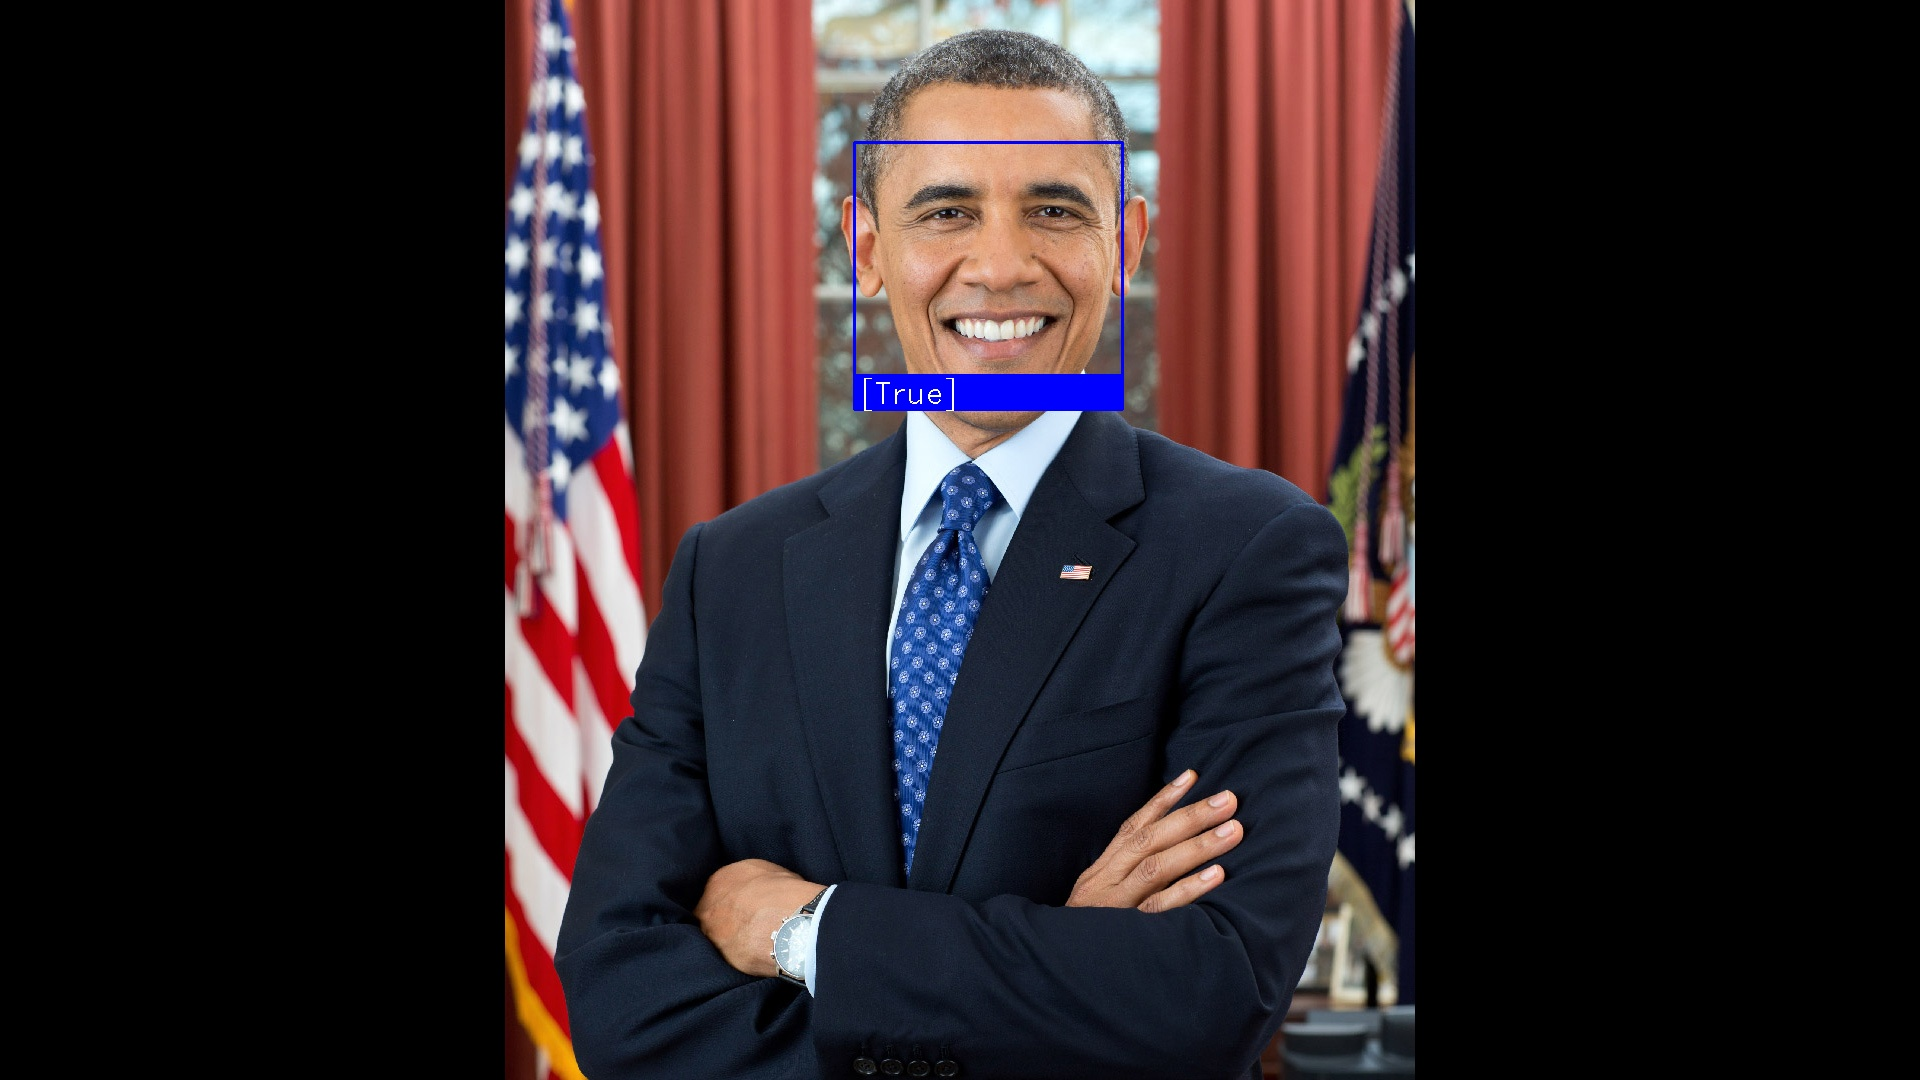
\includegraphics[width=60mm, keepaspectratio]{03_images/obama/o-obama-1080p.jpg}
%	\caption[Minta kép, a felbontás teszteléséhez]{Minta kép, a felbontás teszteléséhez\cite{artc_gold}.}
%	\label{fig:ob_test}
%\end{figure}
%\footnotetext{kép forrása: \url{https://github.com/ageitgey/face_recognition/blob/master/examples/obama-720p.jpg}}

Az \refstruc{fig:res_graphs} mutatja a mérések eredményét. A bal felső grafikonról leolvasható, hogy az arcok helyének megtalálása annál több időt vesz igénybe minél jobb minőségű a kép. Nagyobb felbontás több képpontot jelent, azaz több adatot, ami értelemszerűen nagyobb számítási kapacitást igényel. Mellette az „Enkódolás képből” grafikon a képből az arc „enkódolásának” kinyeréséhez szükséges időt mutatja be. A „Arcvonások” grafikon az arcvonások számosítása során eltelt időt ábrázolja. Az arcok „enkódolását” úgy is ki lehet nyerni a képekből, ha először lefuttatjuk az arcok helyeinek megkeresését, és aztán a helyeket tartalmazó listát is átadjuk az arcokat „enkódoló” függvény számára. Ennek a futásidejét a „Encodings from locations” grafikon mutatja be. Az ábrákból levonható következtetés, hogy amit befolyásol a kép felbontása, az az arcok helyének megtalálása. A két baloldali grafikonból jól látható, hogy amikor már előzetesen megkerestük az arcok helyét, a nagyobb felbontás nem eredményezett láthatóan több futásidőt. A teszt eredeti kimenete a mellékletekben megtalálható(\ref{lst:res_mel}).
\begin{figure}[!ht]
	\centering
	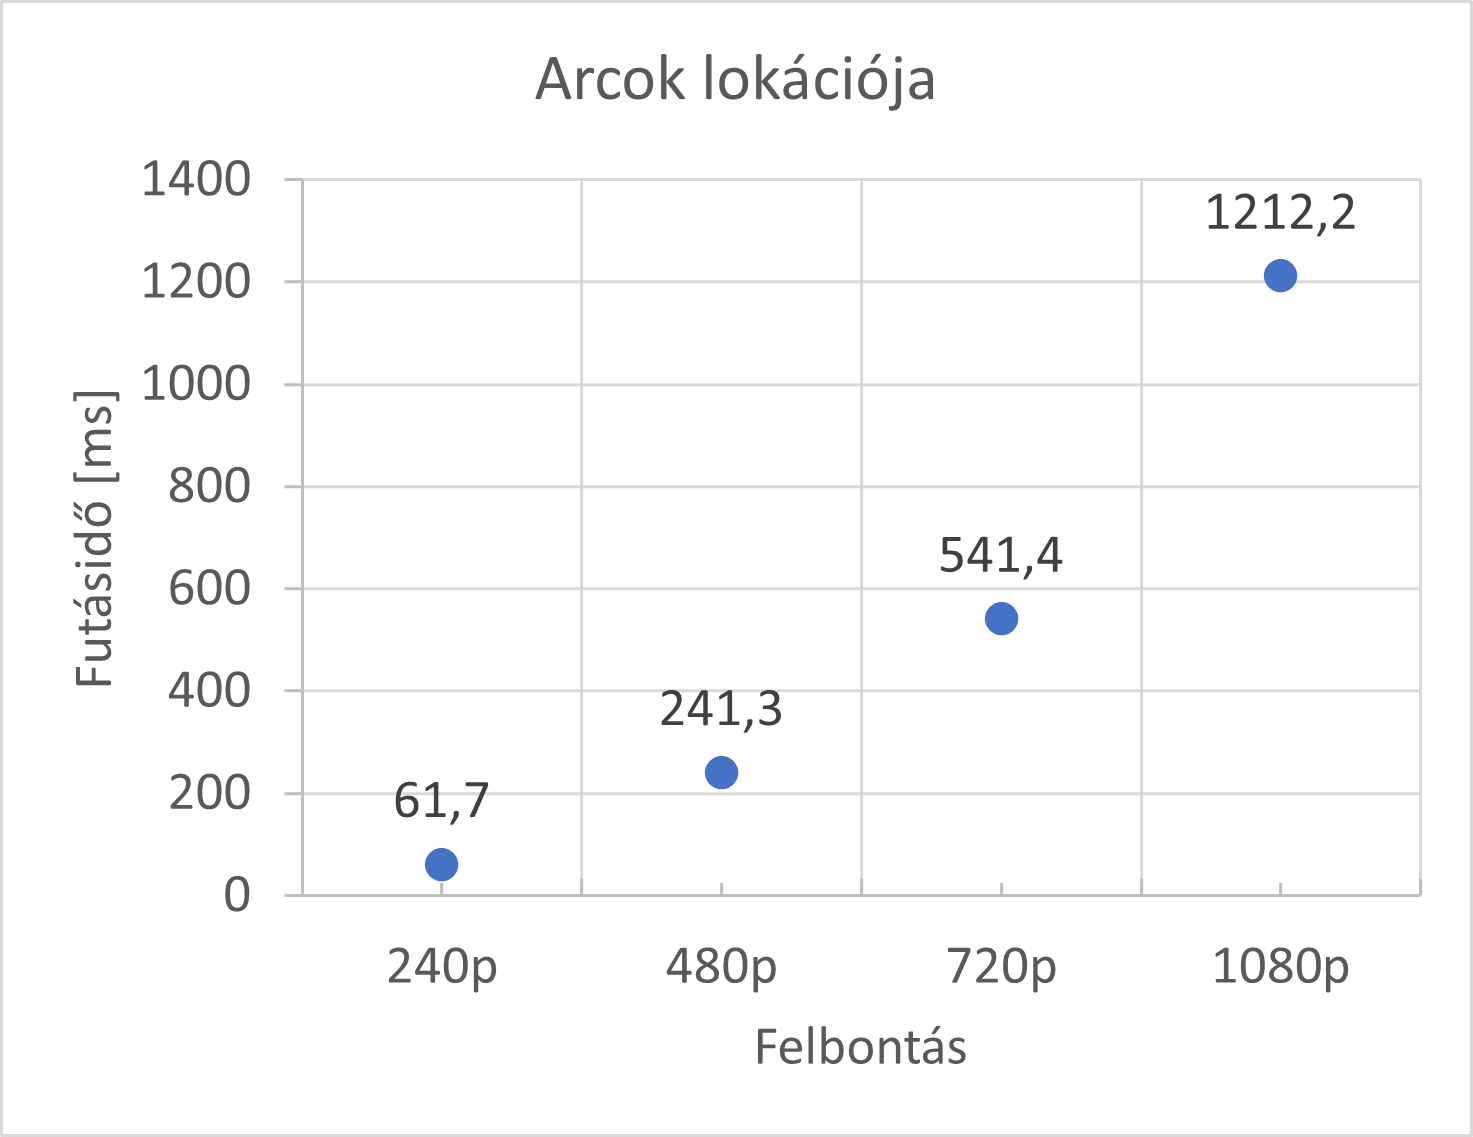
\includegraphics[width=67mm, keepaspectratio]{03_images/graph2/mennyiseg1.png}\hspace{1cm}
	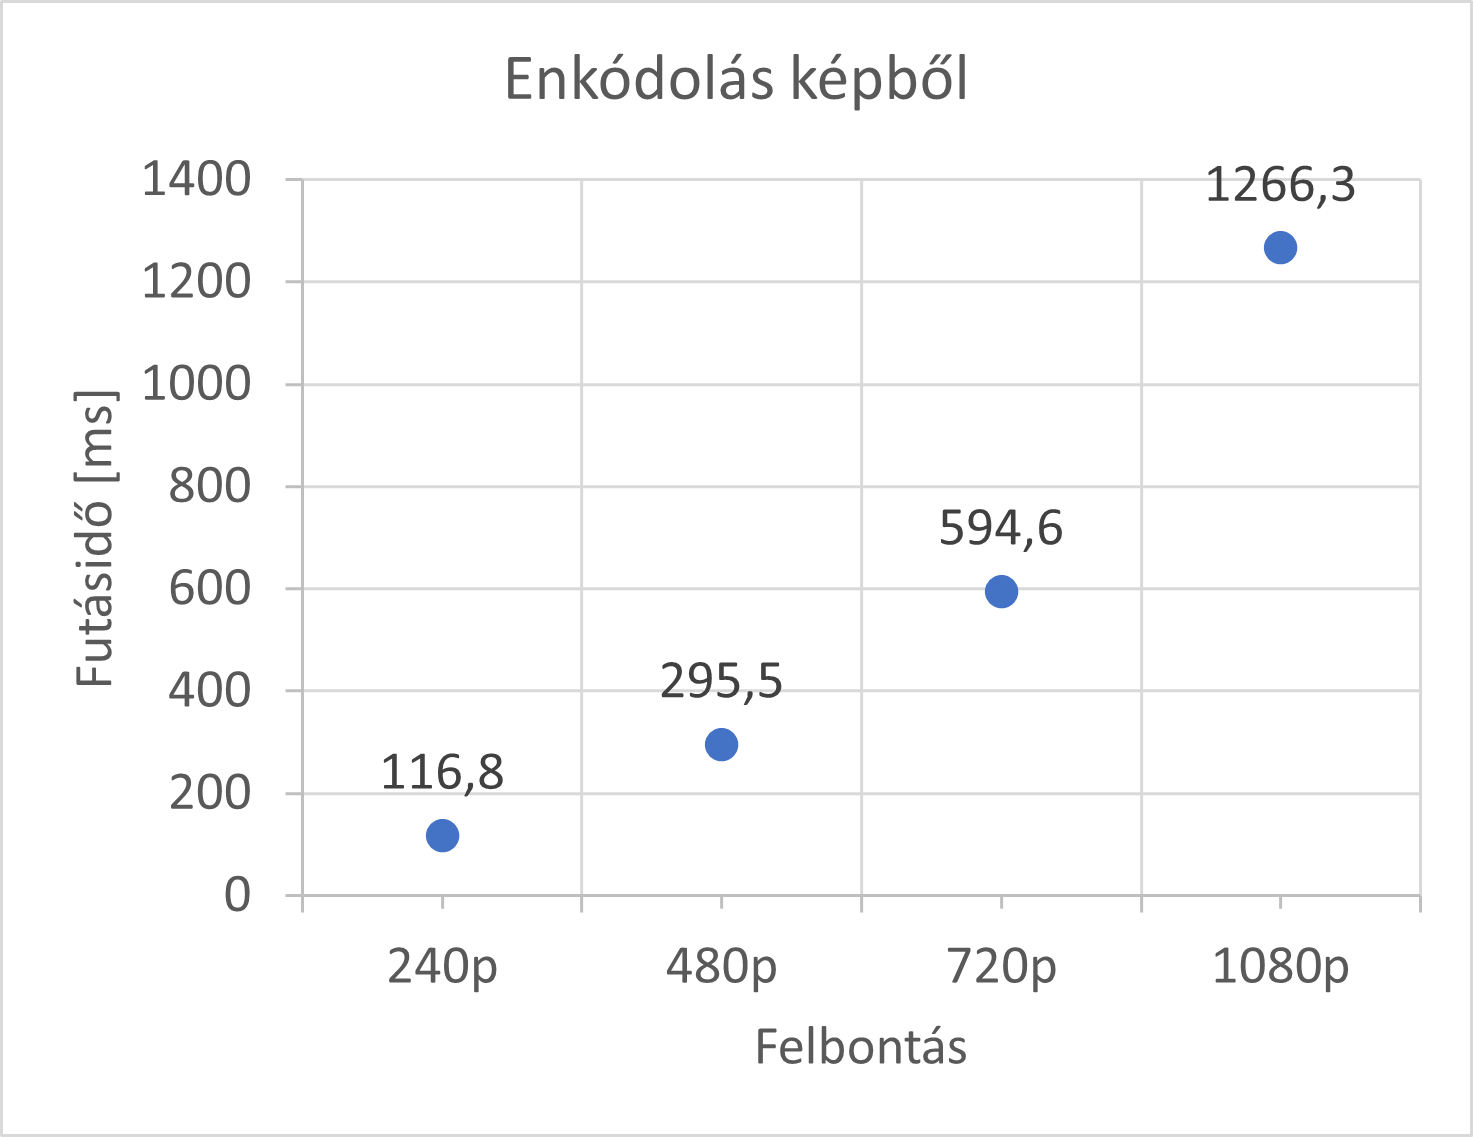
\includegraphics[width=67mm, keepaspectratio]{03_images/graph2/mennyiseg12.png}\\\vspace{5mm}
	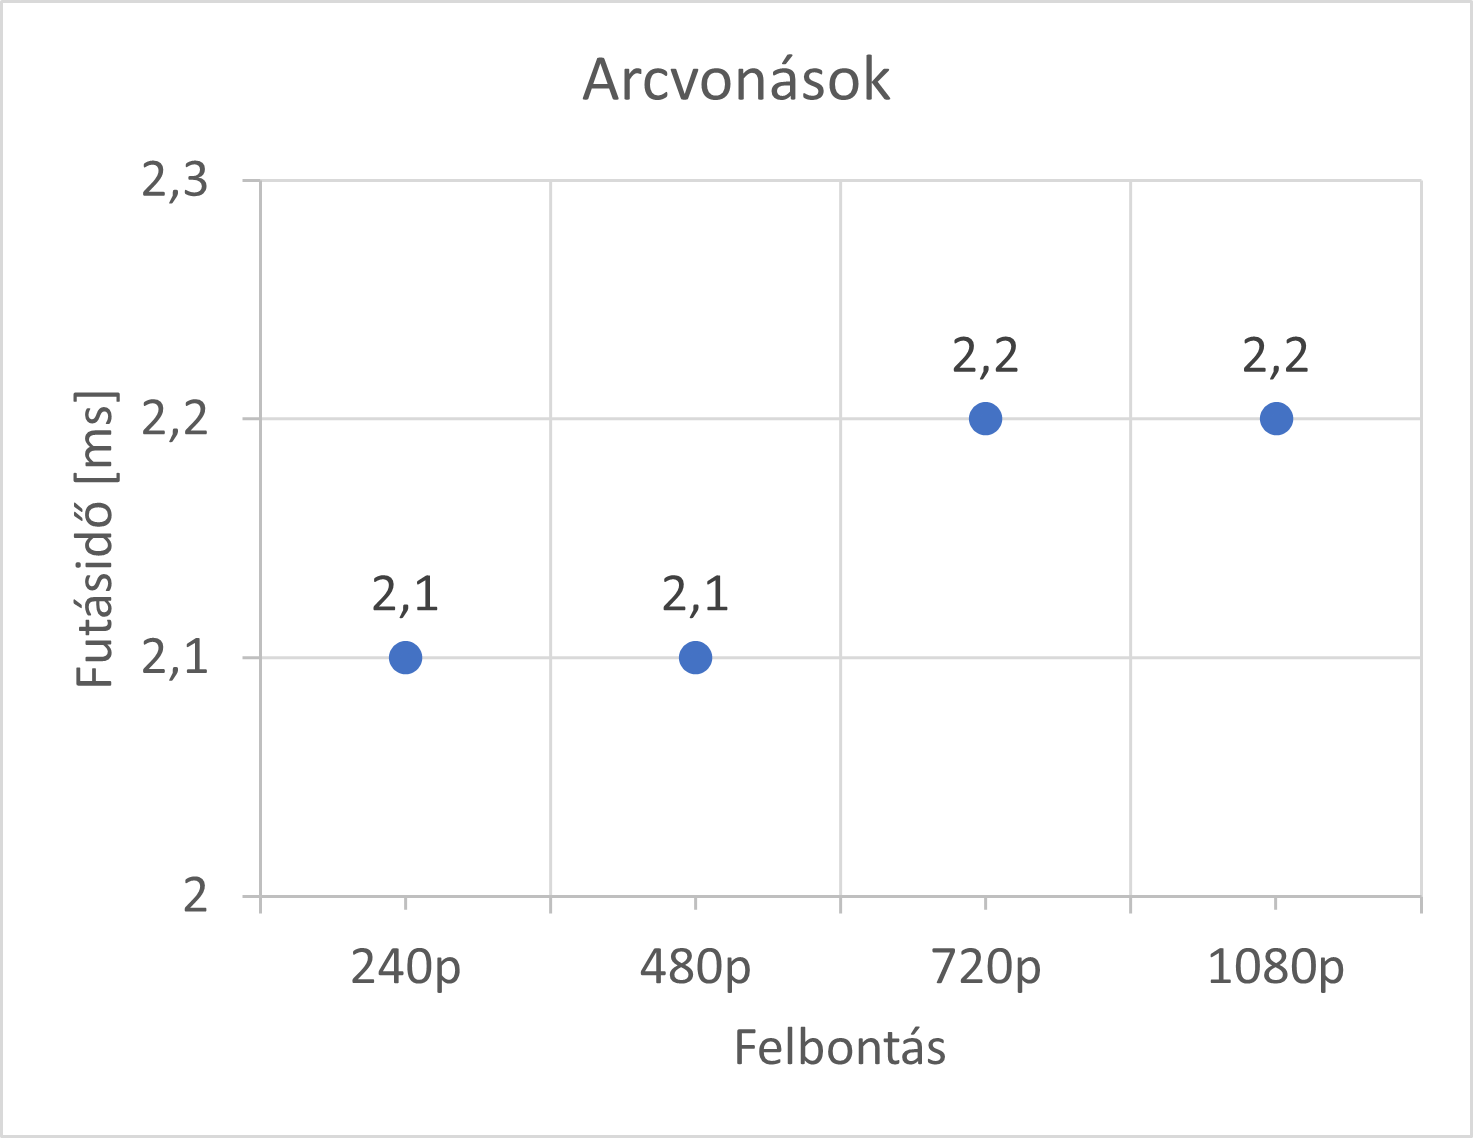
\includegraphics[width=67mm, keepaspectratio]{03_images/graph2/mennyiseg123.png}\hspace{1cm}
	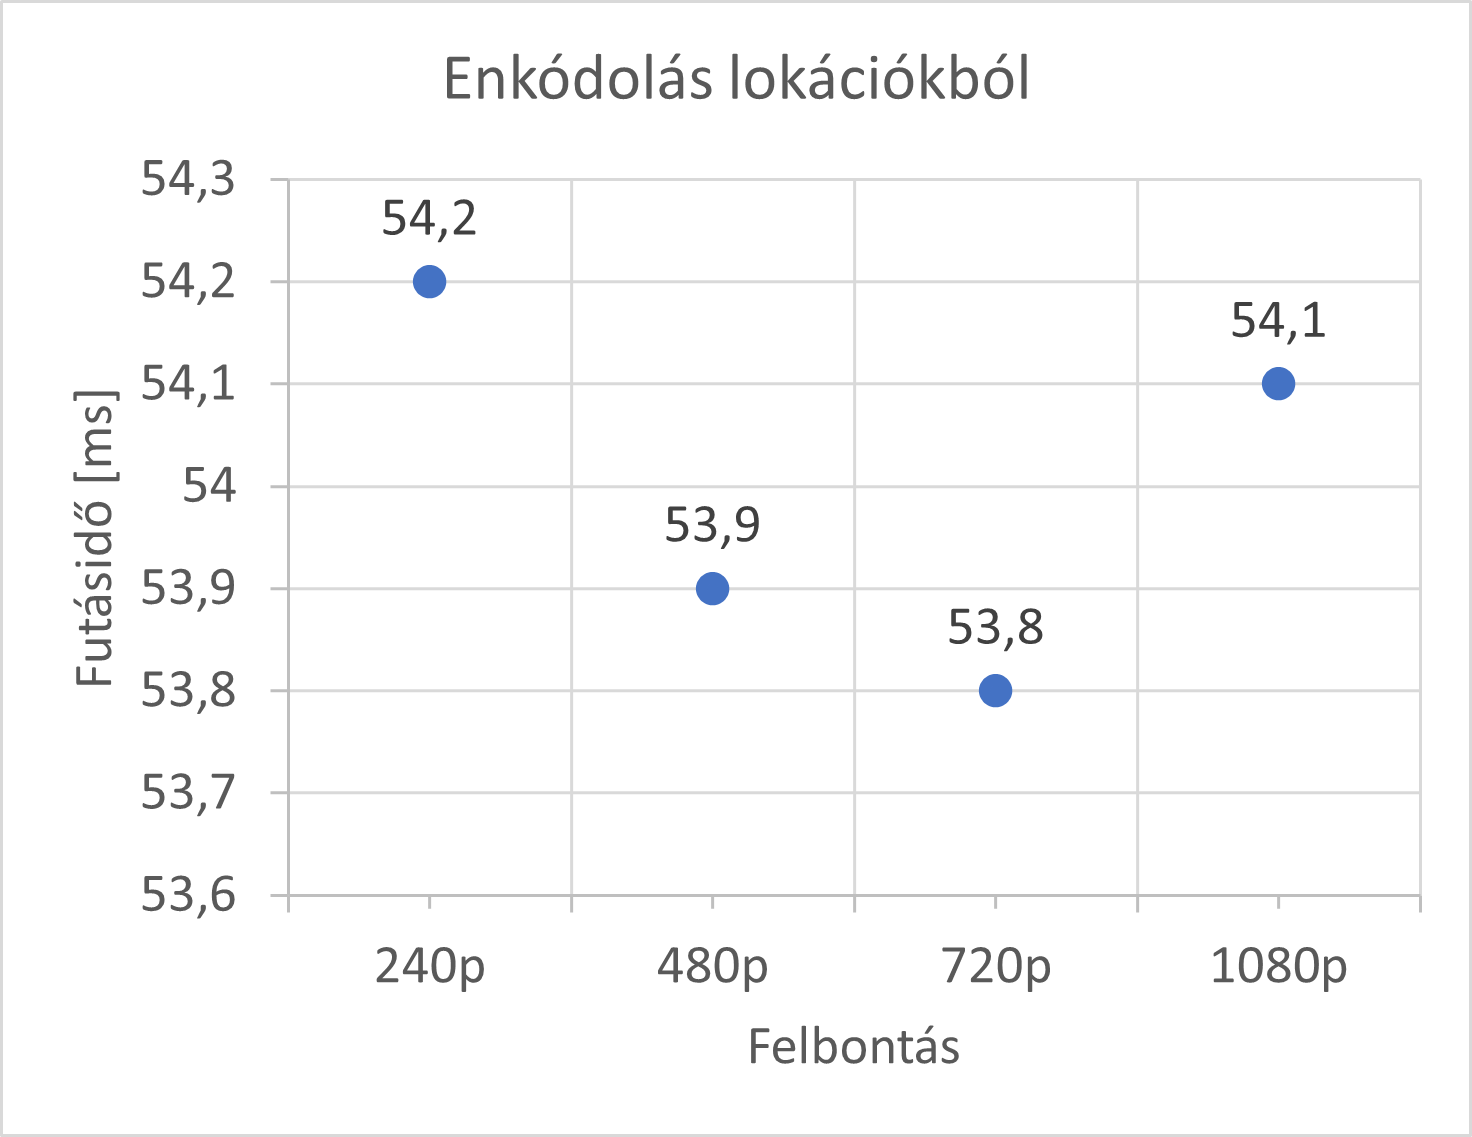
\includegraphics[width=67mm, keepaspectratio]{03_images/graph2/mennyiseg1234.png}
	\caption{Grafikonok a felbontás teszt eredményeiről.}
	\label{fig:res_graphs}
\end{figure}



 \clearpage
\section{Orientáció teszt}
% https://fei.edu.br/~cet/facedatabase.html
Valós alkalmazásban gyakran előfordulhat, hogy az emberek nem néznek bele frontálisan a robot kamerájába, ezért szükséges, hogy a szoftver képes legyen különböző orientációkban is felismerni arcokat. Ebben a mérésben a „FEI Face Database”\cite{artc41}-ből vett képeket elemeztem. Az mellékletben található \refstruc{fig:ori_test} bemutatja, hogy széles horizontálisan változó fej orientációs spektrumon képes az algoritmus arra, hogy felismerjen emberi arcokat.

A mérés során lefuttatott tesztek eredménye a mellékletben található: \ref{lst:ori_mel}. A kapott adatok szemléltetésére készítettem a lenti grafikonokat (\refstruc{fig:ori_graphs}). A minta arcnak, amihez hasonlítottam a különböző képeket egy olyat válsztottam, melyen a személy a kamerába néz. A vizsgált képek mérete és felbontása megegyezik. A grafikonokról megállapítható, hogy az elforgatott arcok nem befolyásolják se az arc helyének megkeresésére fordított időt, se az „enkódolásra” fordított időt. 
\begin{figure}[!ht]
	\centering
	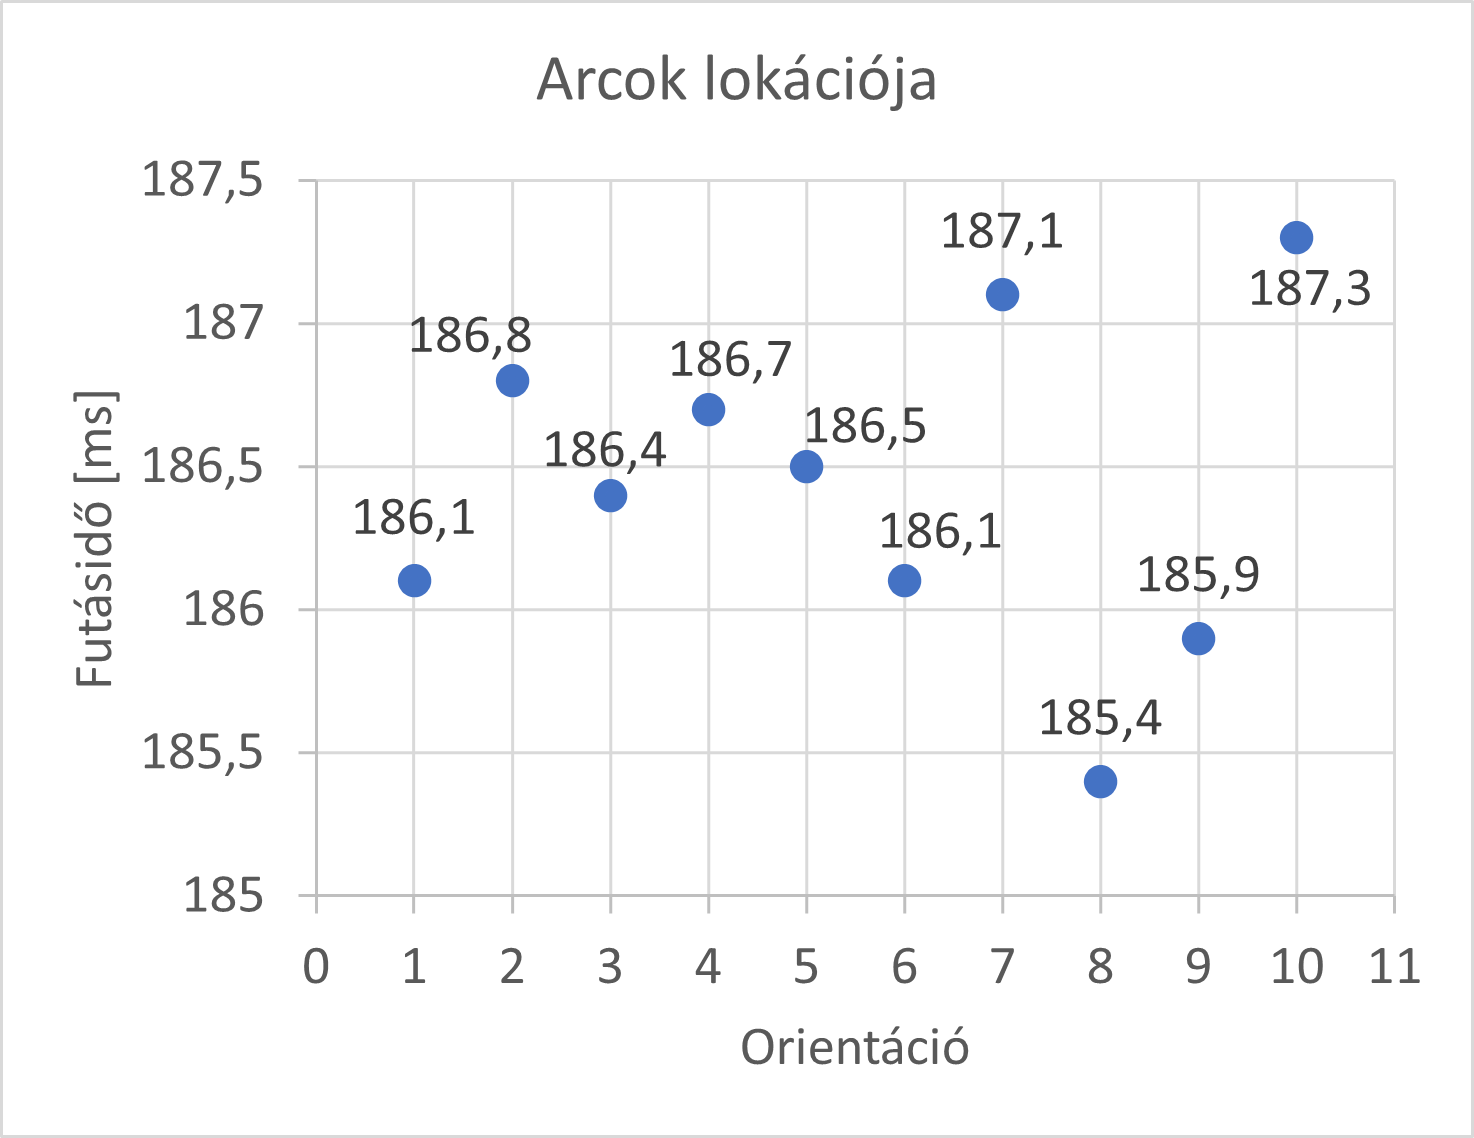
\includegraphics[width=67mm, keepaspectratio]{03_images/graph2/orientacio.png}\hspace{1cm}
	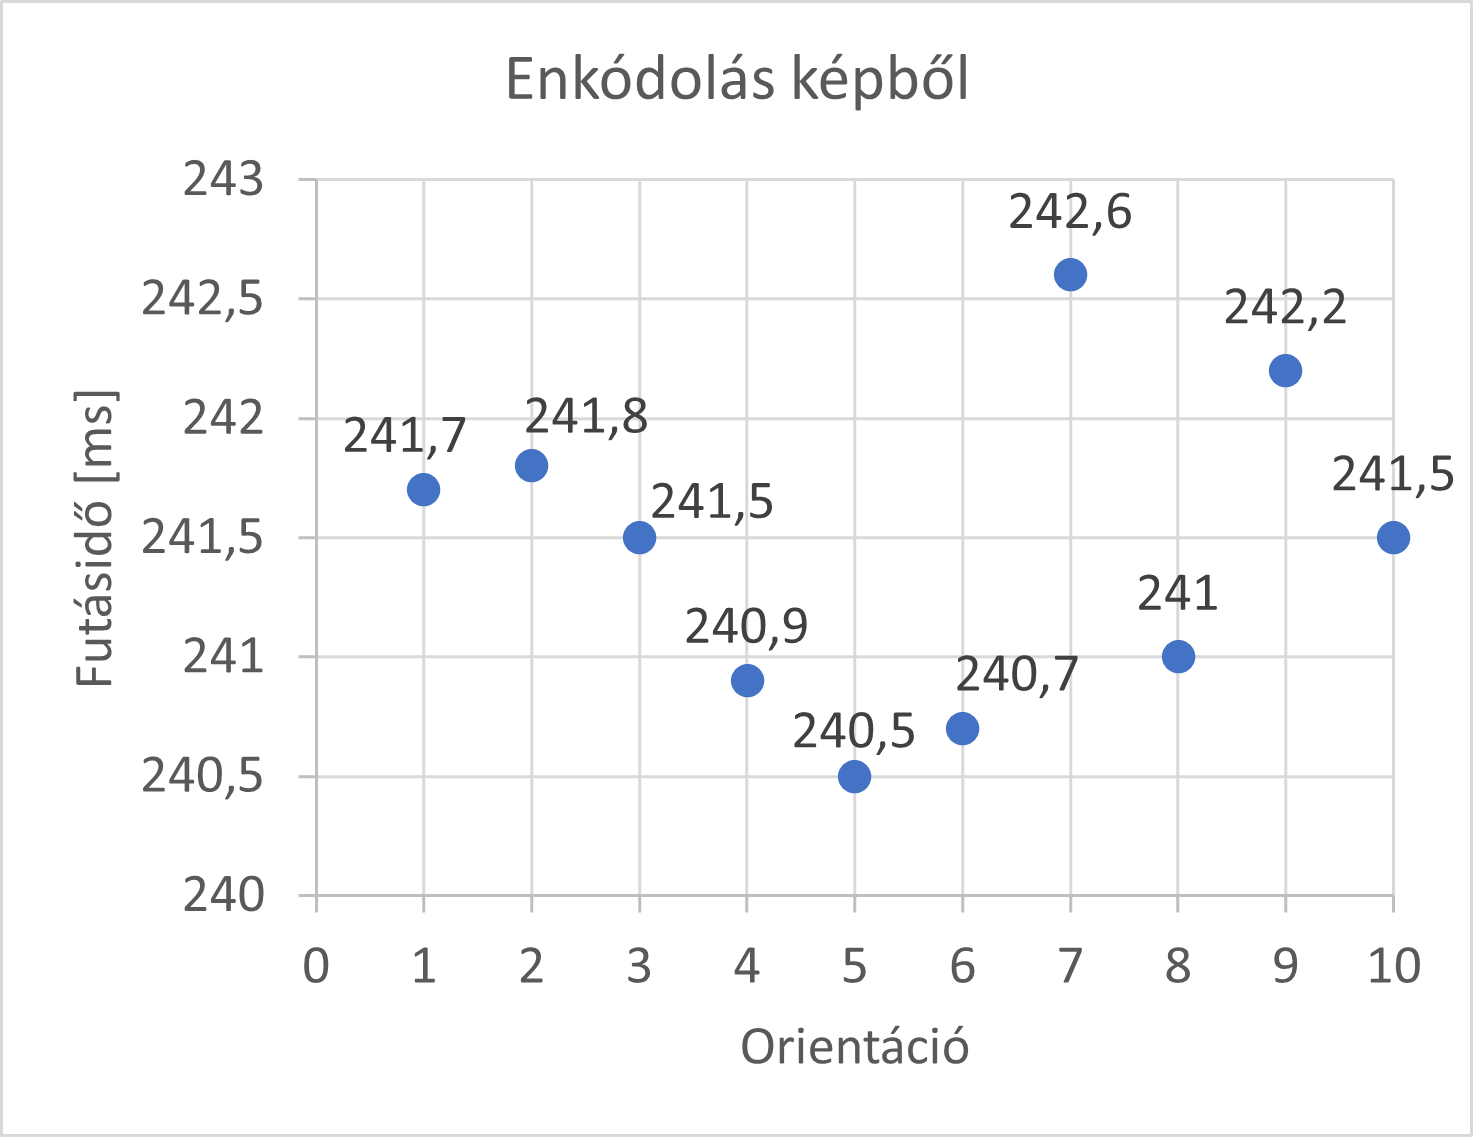
\includegraphics[width=67mm, keepaspectratio]{03_images/graph2/orientacio2.png}\\\vspace{5mm}
	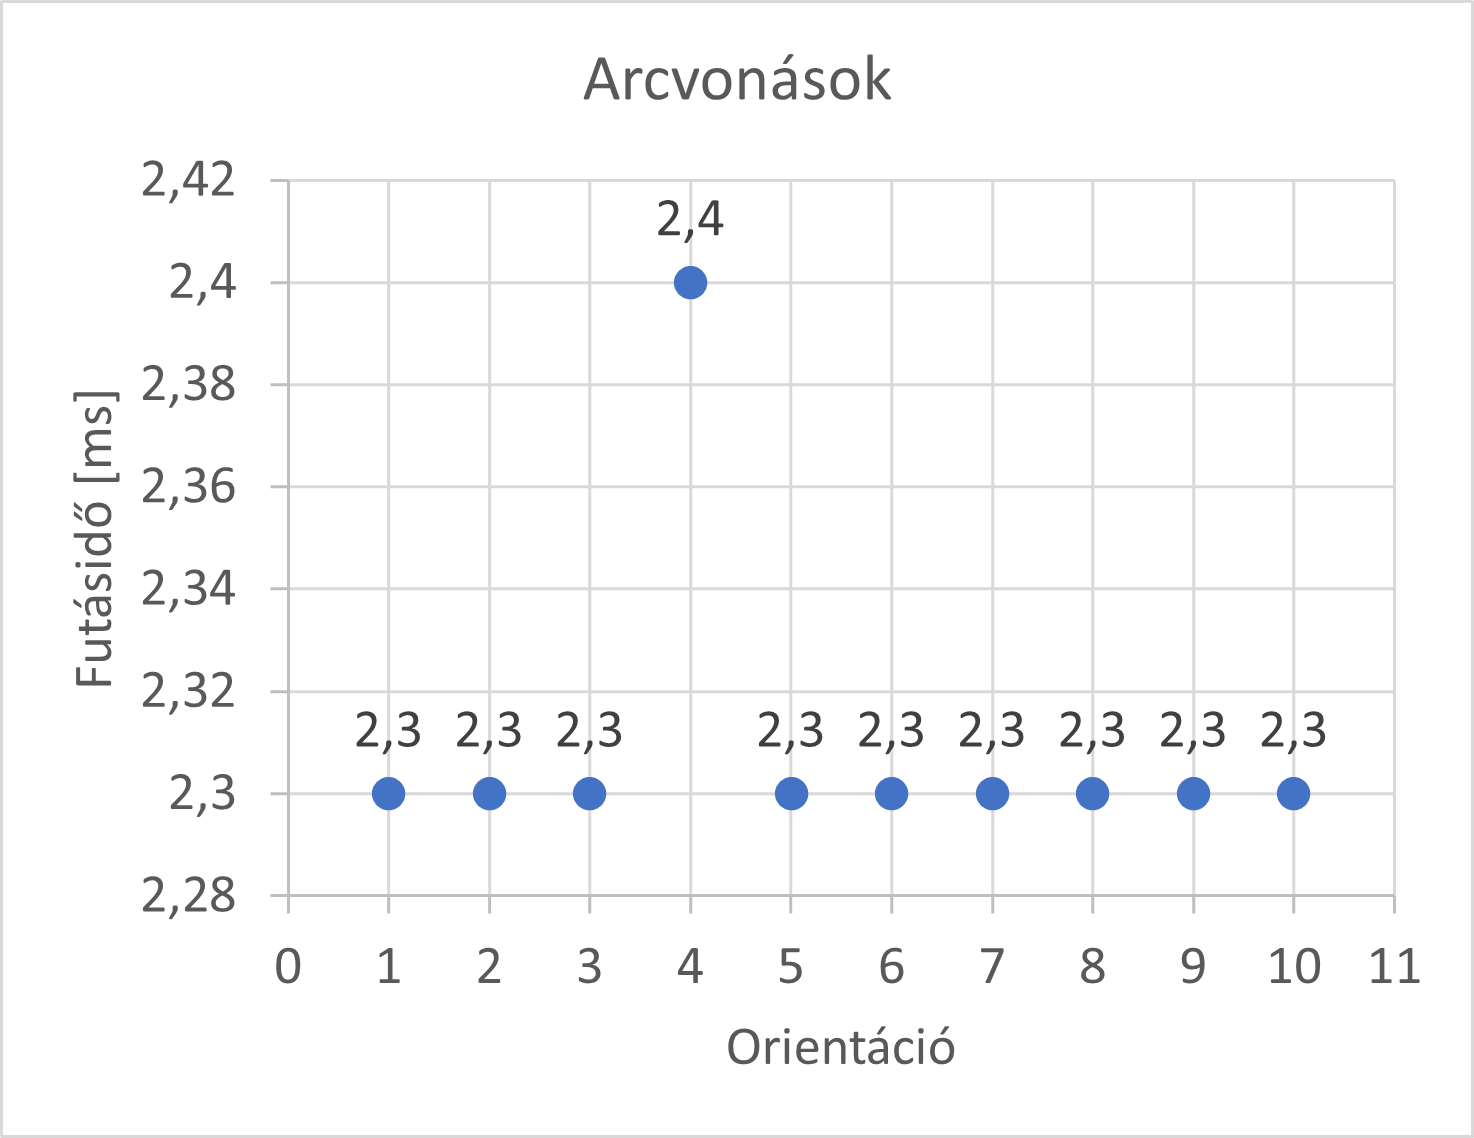
\includegraphics[width=67mm, keepaspectratio]{03_images/graph2/orientacio3.png}\hspace{1cm}
	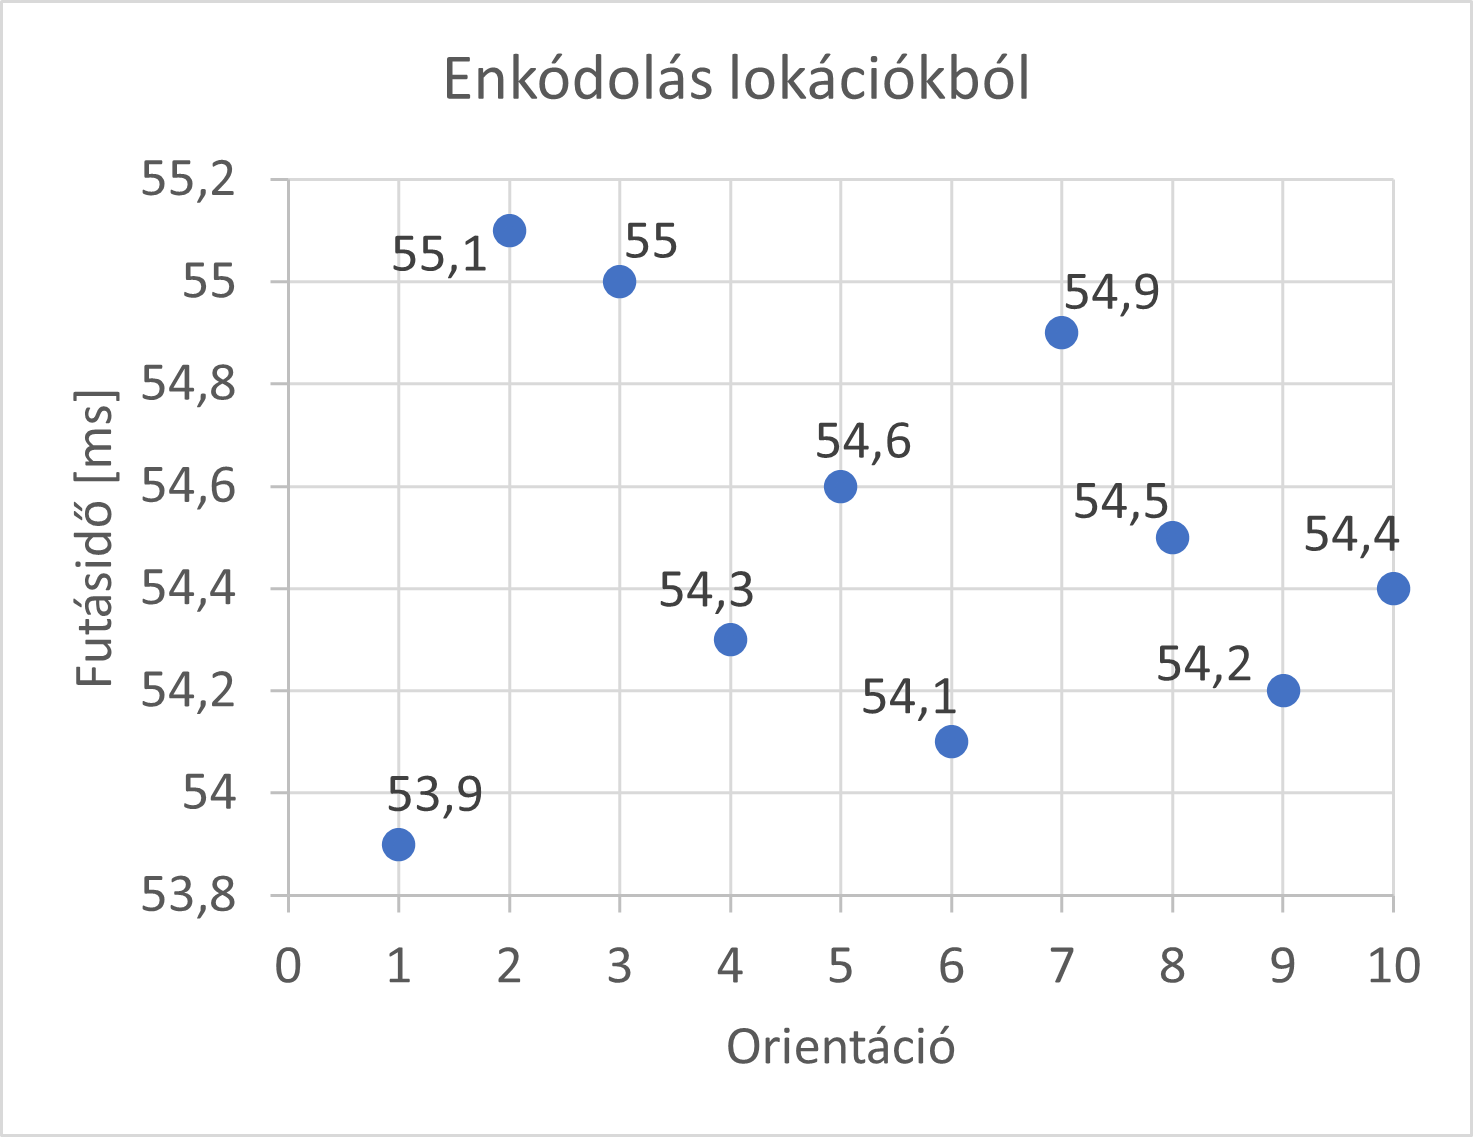
\includegraphics[width=67mm, keepaspectratio]{03_images/graph2/orientacio4.png}
	\caption{Grafikonok az orientáció teszt eredményeiről.}
	\label{fig:ori_graphs}
\end{figure}
%----------------------------------------------------------------------------
\chapter{\osszefoglalas} % (Eredmények értékelése)
%----------------------------------------------------------------------------


\section{Eredmények}
A személyfelismerő rendszer implementálása mobil szociális robotra olyan technológiai megoldás, mellyel lehetővé válik a robot számára, hogy azonosítsa az embereket és kapcsolatba lépjen velük egyéni módon. A mobil szociális robotok komplex gépek, melyek jellemzően képesek mozogni és navigálni környezetükben és emberekkel interakcióba lépni. Különböző feladatokat és szolgáltatásokat láthatnak el emberek életterében, ezért szükséges, hogy érzékeljék a mellettük létező, mozgó embereket. A robotok különböző módokon érzékelhetik az embereket. Az egyik legelterjedtebb megoldás, hogy kamerákkal szerelik fel őket és számítógépes látást használva azonosítanak embereket. A szakdolgozatomban én is egy ilyen megoldást választottam, tekintettel a cél robot: Biscee jelenlegi szenzoraira. A mobil szociális robotok olyan robotok, amelyek képesek kommunikálni és interakcióba lépni az emberekkel. A személyreszabott interakció feltétele, hogy képes legyen felhasználók megkülönböztetésére, ezért az emberek észlelése mellett fontos a felismerésük is. A technológia, amit a projekt során válsztottam az emberek felismerésére az arcon alapuló szemyélyfelismerés.

Az arcfelismerés egy olyan technológia, amely képes azonosítani az emberek arcát digitális képek vagy videók segítségével. Gyorsabb és hatékonyabb módszer a személyek azonosítására, mint például az írisz- vagy ujjlenyomat-felismerés. Biztonságosabb módszer a személyek azonosítására, mint például a jelszavak használata, mert az arcot nem lehet könnyen meghamisítani. Széles körben elérhető, és általában nem igényel különleges eszközöket vagy berendezéseket. Egyszerűen használható, mert az embereknek csak a saját arcukat kell megmutatniuk a kamera előtt, és nem kell bonyolult jelszavakat vagy más adatokat megadniuk.

A feladatom egy személyfelismerő rendszer létrehozása volt. Két felhasználási célt határoztunk meg a Biscee roboton. Az első, hogy manuálisan betanított adatokból képes legyen ember felismerésére. A második, hogy újonnan látott embereket is megjegyezzen, későbbi találkozás során emlékezzen rájuk. A létrehozott csomagot úgy alkottam meg, hogy mindkettő feladatot ellása. Képfájlokat adhatunk meg, amiken észlelt arcokat jegyez meg, hozzájuk nevet is társíthatunk. Futás során a kamerán megjelenő arcokat megjegyzi és elmenti. 

A Biscee robottal több olyan, valódi élethelyzetekben végzett kísérletet tervezünk, ahol a robot pincérsegédként működve felismerheti az emberi pincéreket, illetve egyetemi és irodai környezetben az ott dolgozókat. A személyfelismerés kialakítása Bisceen nem csak azt teszi lehetővé, hogy a robot eltérően viselkedjen az ismerős és a még ismeretlen személyekkel, de elősegíti az adatgyűjtést és az autonóm kiértékelést is a kísérleteknél.

A projekt célja egy ROS csomag fejlesztése volt Noetic verzió alatt, ami magában foglal egy
kamera kezelő „node"-ot, egy adatbázis „node"-ot és egy, az arcok felismerését ellátó „node"-ot. Az arcfelismerést a „face-recognition" Python modul használatával kiviteleztem, ami egy fejlesztőként könnyen használható könyvtár. Dlib-re épült konvolúciós hálót alkalmazva, az emberi arcokról „enkódolást" készít, ami egy 128 elemű listával írja le az arcok tulajdonságait. A létrehozott „enkódolás" számítógép számára értelmezhetővé teszi (kvantálttá) a személyek arcait, így összehasonlíthatóvá válnak. Az „enkódolások" 128 dimenziós vektorként értelmezhetők euklidészi térben, távolságot számítva közöttük megállapítható az arcok eltérése vagy egyezése. Az arcokhoz társított adatokat: név, „id" és „enkódolás" adatbázisban tárolja, ennek menedzselésére létrehoztam egy külön osztályt, ami a Pandas \verb|Dataframe| osztályára épült. A kamera képéről észlelt arcokat képes a csomag összehasonlítani az adatbázisban tárolt személyek arcaival. Az észlelt és felismert embereket megjelöli az élő képen. 

\section{Javaslatok} % Válassz egyet
A csomag fejlesztése közben több területen gondolkodtam a további bővítési lehetőségeken. Az adatbázis struktúra felé, az objektum orientált programozás koncepcióját szem előtt tartva, bővíthető a csomag egy osztállyal. Úgy gondolom hasznos lenne egy struktúrába szervezni az arcokhoz tartozó adatokat, mely így megvalósítható lenne.

A Biscee robotra való telepítés még egy fontos feladat, mely során figyelembe kell majd venni a robot hardveres erőforrásait. A feldolgozás folyamatának számos paraméterét be kell kalibrálni, hogy valós idejű rendszerként tudjon működni. Ezen paraméterek alatt értem a kamera képének felbontását, másodpercenkénti elkészített képek számát (FPS), az arcok felismerésben fontos szerepet játszó tolerancia értékének megválasztását. Mindezen változók, tényezők kalibrálása további teszteket igényel.

Az arcok feldolgozásának folyamata annál több időt vesz igénybe, minél több arccal kell összehasonlítanunk. Mivel a csomag folyamatosan tanulja meg új emberek arcait, ezért az adatbázis könnyen nagy méretűvé tud válni, főleg akkor, ha a robotot egy forgalmas helyen alkalmazzuk. A nagy adathalmaz megnöveli az újonnan látott arcok feldolgozásásának idejét. Ebből az elgondolásból hoztam létre egy „cache" adatbázist, amiben megadhatók azok a személyek, akiket a robot potenciálisan többször lát (például pincérek vagy dolgozók). Ez azért gyorsítja a feldolgozást, mert először ebben az adatbázisban keres egyezést az algoritmus és csak ez után tér át a fő adathalmazra. További optimalizáció céljából egy lehetséges fejlesztés, hogy elmentsük az előző képkockán látott arcokat és új kép beérkezésekor először ezeket az elmentett adatokat vizsgáljuk. Valós felhasználás alkalmával előreláthatólag több ideig tartózkodnak emberek a kamera látóterében, ezért több egymásutáni képkockán is meg fog jelenni az arcuk. Viszont egy képkockán kézenfekvően nem lesz akkora embertömeg jelen, hogy hatalmas adathalmazt generáljon belőlük az algoritmus, ezért ha alkalmazzuk a leírt fejlesztést, csak egy kis méretű listát kell először átvizsgálni arcfelismerés során. A kisebb adatbázison gyorsabban végez feldolgozást, ezért összességében megállapítható, hogy gyorsítani tudná a teljes arcfelismerés folyamatát.

% Keltezés, aláírás
\vspace{0.5cm}

\begin{flushleft}
{Budapest, \today}
\end{flushleft}

\begin{flushright}
\emph{\authorName}
\end{flushright}

\vfill



% Bibliográfia [Bibliography]
\addcontentsline{toc}{chapter}{\bibname}
{
    \footnotesize  % Kisebb betűméret [Smaller font size]
    \bibliography{bib/mybib}
}


% Idegen nyelvű (angol) összefoglaló [Foreign language summary]
%----------------------------------------------------------------------------
\chapter*{\summary}\addcontentsline{toc}{chapter}{\summary}
%----------------------------------------------------------------------------

\selectforeignlanguage % angol (magyar) nyelvi beállítások

Implementing a person recognition system on a mobile social robot is a technological solution that allows the robot to identify and interact with people in a personalised way. Mobile social robots are complex machines that are usually able to move and navigate in their environment and interact with humans. They can perform various tasks and services in people's living space, and therefore need to be able to sense people existing and moving alongside them. Robots can sense people in different ways. One of the most common ways is to equip them with cameras and use computer vision to identify people. For my thesis, I chose such a solution, given the current sensors of the target robot: Biscee. Mobile social robots are robots that can communicate and interact with humans. A prerequisite for personalized interactions is the ability to distinguish users, so in addition to detecting people, it is also important to recognize them. The technology that I have developed for this project to recognise people is based on face recognition.

Face recognition is a technology that can identify people's faces using digital images or videos. It is a faster and more effective method of identifying people than, for example, iris or fingerprint recognition. It is a more secure method of identifying people than, for example, using passwords, because a face cannot be easily faked. It is widely available and does not usually require special tools or equipment. Simple to use because people only need to show their face to the camera and do not need to provide complex passwords or other information.

The aim of the project was to develop a ROS package under the Noetic version, which includes a camera management node, a database node and a face recognition node. I implemented the face recognition using the Python module "face-recognition", which is a library that is easy to use as a developer. Using a convolutional mesh built on Dlib, it generates an encoding of human faces, which describes the properties of the faces with a 128-item list. The generated encoding makes the faces of persons interpretable (quantized) by a computer, so that they can be compared. The encodings are interpreted as 128 dimensional vectors in Euclidean space, and by calculating distances between them, the difference or similarity of the faces can be determined. The data associated with the faces: name, id and encoding is stored in a database, and I also created a separate class to manage it, based on the \verb|Dataframe| class of Pandas. The package is able to compare the faces detected from the camera image with the faces of the persons stored in the database. The detected and recognized people are marked on the live image.



\vspace{0.5cm}
\paragraph{Keywords} \emph{\keywords}  % A kulcsszavak a fő tex fájlban vannak definiálva


\selectthesislanguage % térjünk vissza magyar (angol) nyelvre



% Függelék és mellékletek [Appendices]
%\excludeFromLocAndLot % A következő ábrákat és a táblázatokat hagyja ki a jegyzékből
                      % [Exclude following figures and tables from List Of Figures/Tables]

%%----------------------------------------------------------------------------
\appendix
%----------------------------------------------------------------------------
\chapter*{\fuggelek}\addcontentsline{toc}{chapter}{\fuggelek}
%----------------------------------------------------------------------------
\setcounter{chapter}{\appendixletter} % F betű
%\setcounter{equation}{0}
\numberwithin{equation}{section}
\numberwithin{figure}{section}
\numberwithin{lstlisting}{section}
%\numberwithin{tabular}{section}


% Ismertető - töröld ki
%----------------------------------------------------------------------------
A függelék a főszöveget kiegészíti további részletezéssel. Ide kerül minden kiegészítő információ, ami nem tartozik szorosan a feladat témájához. A függelék rendszerint nem önálló dokumentum. A főszöveg általában nem hivatkozik rá. Általában saját munka.

A dolgozat opcionális eleme, csak igény esetén kell használni.
%----------------------------------------------------------------------------

%----------------------------------------------------------------------------
\section{A TeXstudio felülete}
%----------------------------------------------------------------------------
\begin{figure}[!ht]
\centering
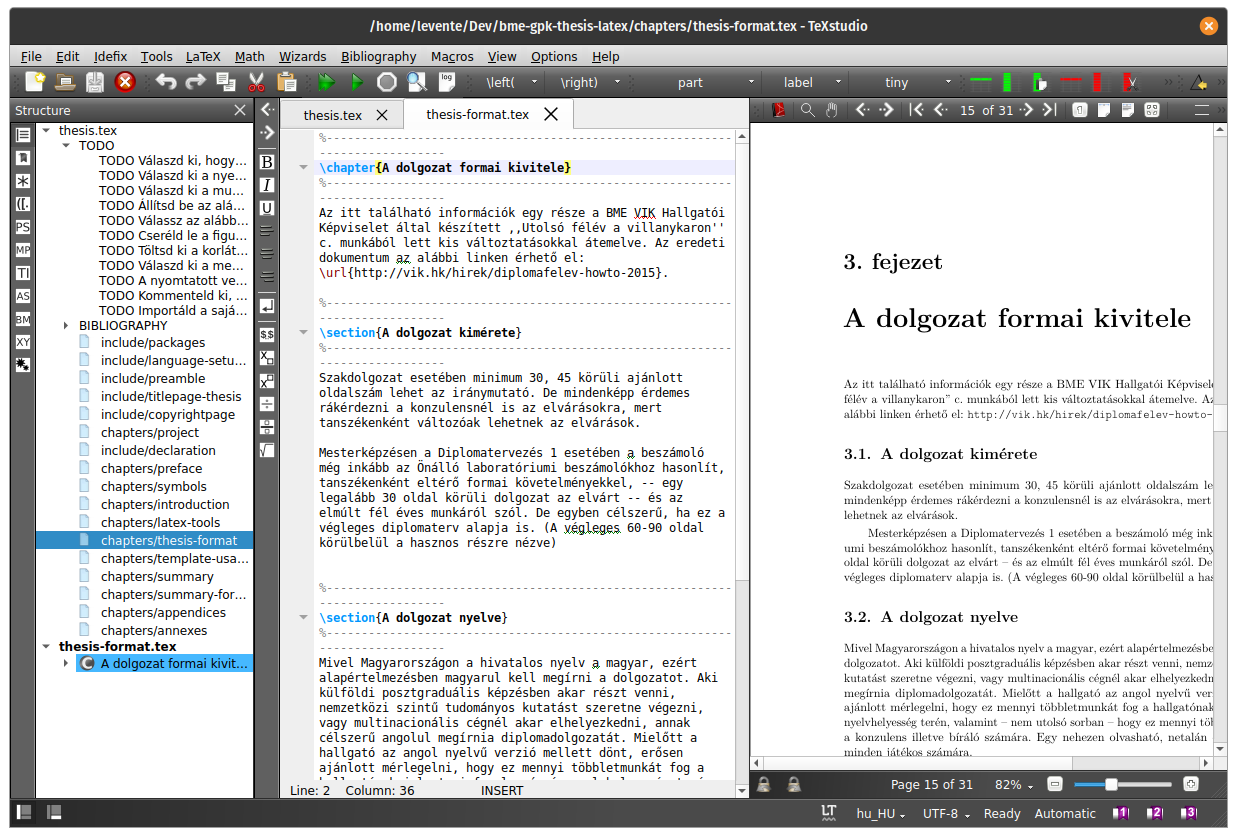
\includegraphics[width=150mm, keepaspectratio]{figures/TeXstudio.png}
\caption{A TeXstudio \LaTeX-szerkesztő.} 
\end{figure}

%----------------------------------------------------------------------------
\clearpage\section{Válasz az ,,Élet, a világmindenség, meg minden'' kérdésére}
%----------------------------------------------------------------------------
A Pitagorasz-tételből levezetve
\begin{align}
c^2=a^2+b^2=42.
\end{align}
A Faraday-indukciós törvényből levezetve
\begin{align}
\rot E=-\frac{dB}{dt}\hspace{1cm}\longrightarrow \hspace{1cm}
U_i=\oint\limits_\mathbf{L}{\mathbf{E}\mathbf{dl}}=-\frac{d}{dt}\int\limits_A{\mathbf{B}\mathbf{da}}=42.
\end{align}
        % Függelék - opcionális
%----------------------------------------------------------------------------
\appendix
%----------------------------------------------------------------------------
\chapter*{\melleklet}\addcontentsline{toc}{chapter}{\melleklet}
%----------------------------------------------------------------------------
\setcounter{chapter}{\annexletter} % M betű
\setcounter{section}{0}
%\setcounter{equation}{0}
\numberwithin{equation}{section}
\numberwithin{figure}{section}
\numberwithin{lstlisting}{section}
%\numberwithin{tabular}{section}

\section{„Node"-ok működését magyarázó ábrák}
\begin{figure}[!ht]
    \centering
    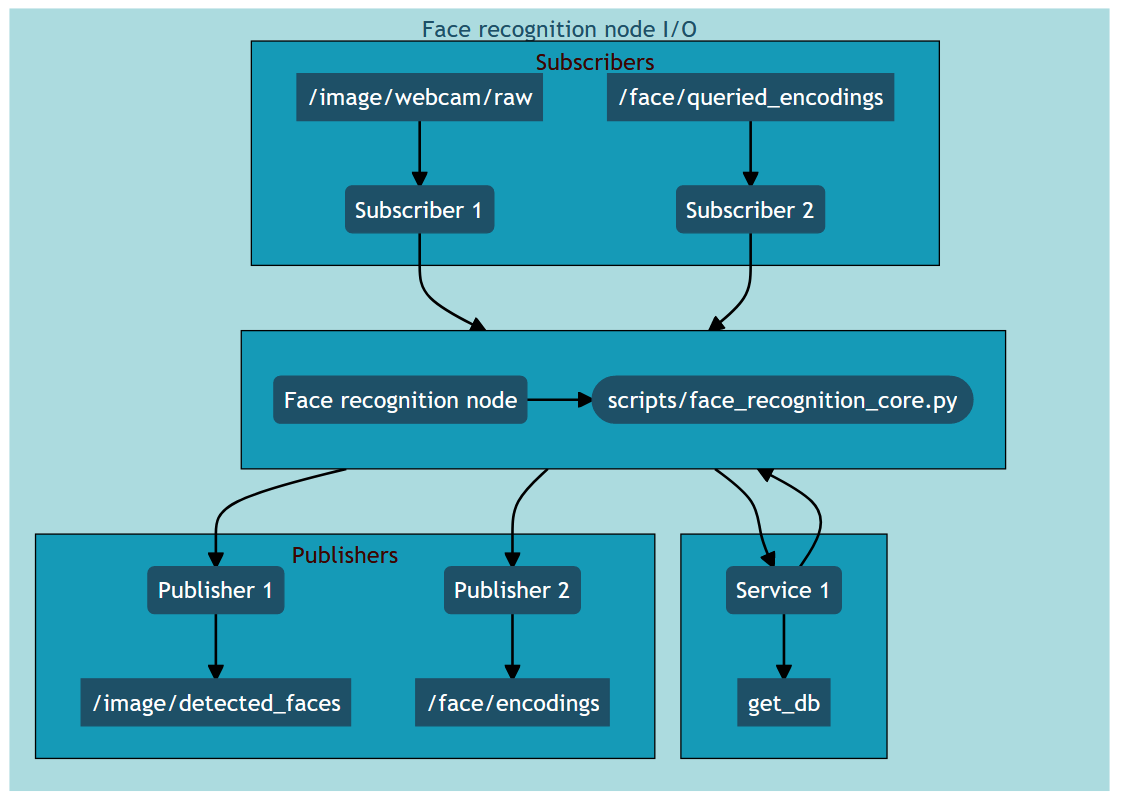
\includegraphics[width=150mm, keepaspectratio]{02_mermaid/facenode2.png}
    \caption{Arcfelismerést végző node „I/O"-ja.}
    \label{fig:frio}
\end{figure}

%----------------------------------------------------------------------------
\clearpage
\section{Felbontás teszt}
%----------------------------------------------------------------------------
\begin{lstlisting}[language=tex, caption=Felbontás teszt eredménye.,label=lst:res_mel]
Timings at resolution 240p:
 - Face locations: 0.0617s (16.20 fps)
 - Face landmarks: 0.0021s (471.55 fps)
 - Encode face (from landmarks): 0.0542s (18.47 fps)
 - Encode face (from image): 0.1168s (8.56 fps)
 - Check for results: 0.0000s (36226.63 fps)
 - Export results: 0.0034s (297.79 fps)

Timings at resolution 480p:
 - Face locations: 0.2413s (4.14 fps)
 - Face landmarks: 0.0021s (469.63 fps)
 - Encode face (from landmarks): 0.0539s (18.56 fps)
 - Encode face (from image): 0.2955s (3.38 fps)
 - Check for results: 0.0000s (35401.24 fps)
 - Export results: 0.0086s (116.53 fps)

Timings at resolution 720p:
 - Face locations: 0.5414s (1.85 fps)
 - Face landmarks: 0.0022s (462.77 fps)
 - Encode face (from landmarks): 0.0538s (18.60 fps)
 - Encode face (from image): 0.5946s (1.68 fps)
 - Check for results: 0.0000s (34976.53 fps)
 - Export results: 0.0172s (58.20 fps)

Timings at resolution 1080p:
 - Face locations: 1.2122s (0.82 fps)
 - Face landmarks: 0.0022s (461.25 fps)
 - Encode face (from landmarks): 0.0541s (18.48 fps)
 - Encode face (from image): 1.2663s (0.79 fps)
 - Check for results: 0.0000s (34540.88 fps)
 - Export results: 0.0366s (27.32 fps)
\end{lstlisting}

\begin{figure}[!ht]
    \centering
    
\includegraphics[width=67mm, keepaspectratio]{03_images/obama/o-obama-240p.jpg}\hspace{1cm}
    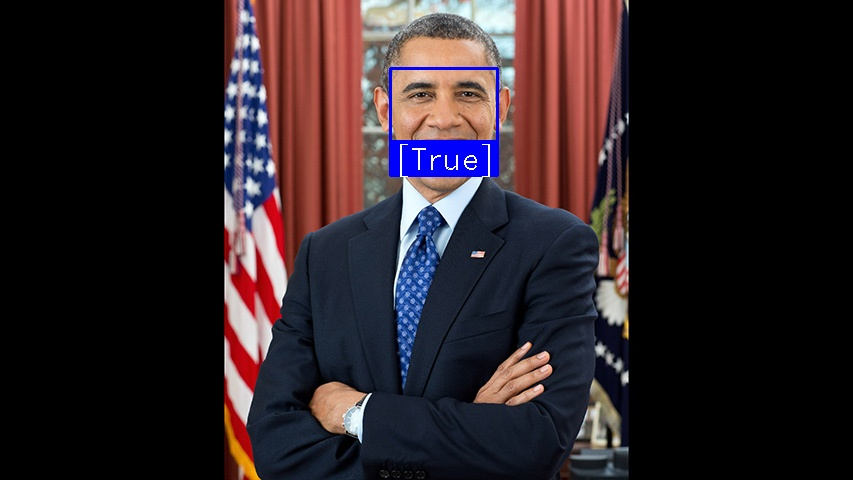
\includegraphics[width=67mm, keepaspectratio]{03_images/obama/o-obama-480p.jpg}\\\vspace{5mm}
    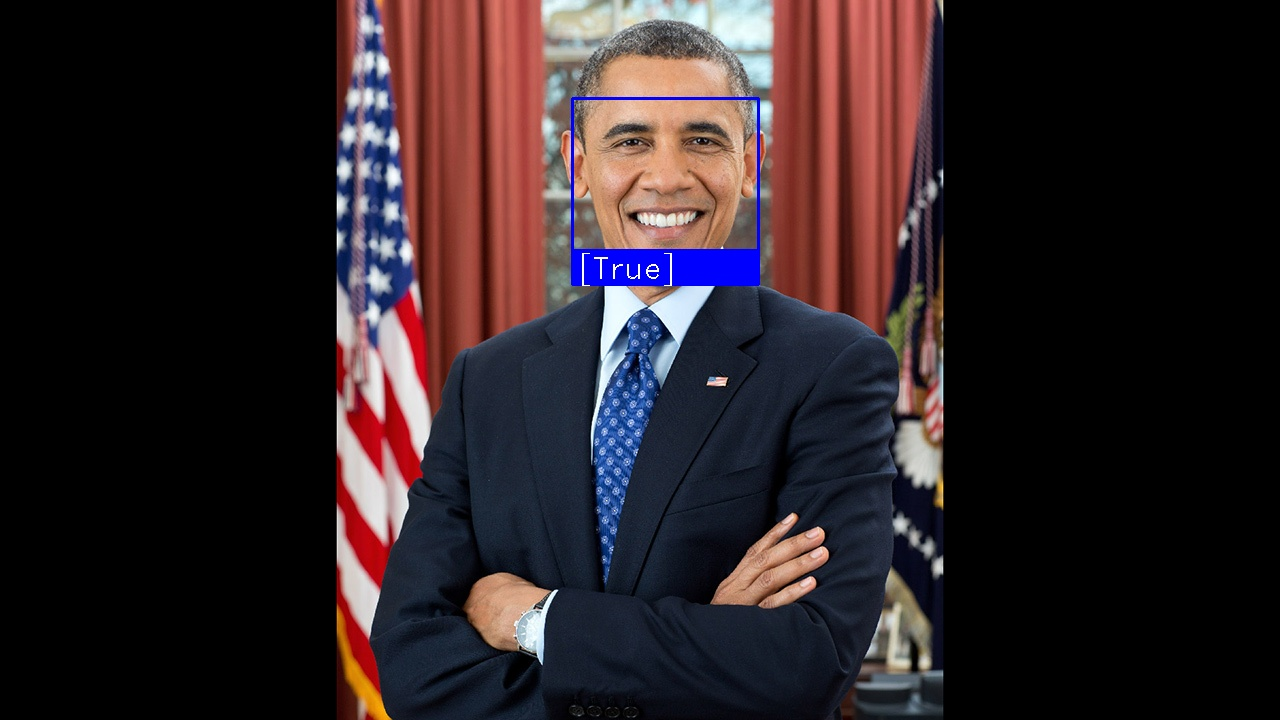
\includegraphics[width=67mm, keepaspectratio]{03_images/obama/o-obama-720p.jpg}\hspace{1cm}
    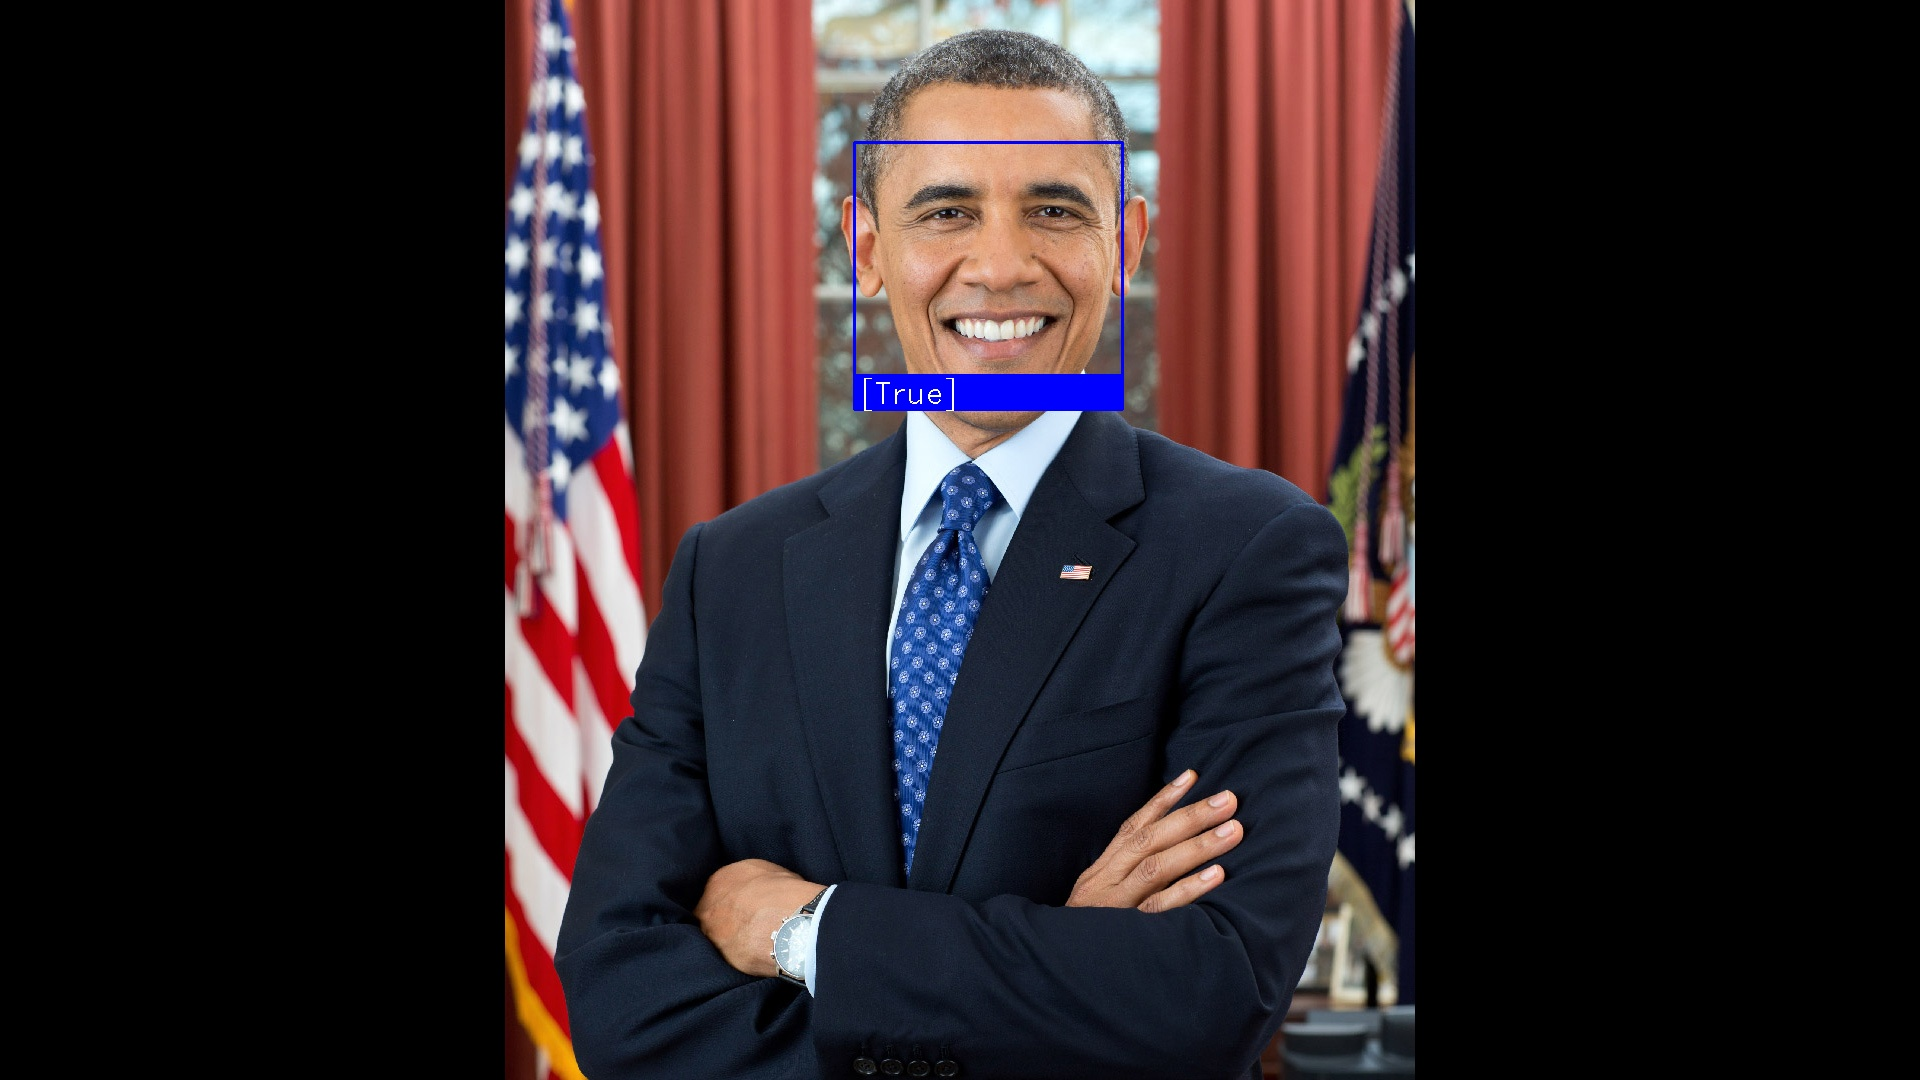
\includegraphics[width=67mm, keepaspectratio]{03_images/obama/o-obama-1080p.jpg}
    \caption{Felbontás teszt eredményei.}
    \label{fig:felbontasteszt}
\end{figure}

%----------------------------------------------------------------------------
\clearpage
\section{Orientáció teszt}
%----------------------------------------------------------------------------

\begin{lstlisting}[language=tex, caption=Orientáció teszt eredménye.,label=lst:ori_mel]
Timings at image 01:
 - Face locations: 0.1861s (5.37 fps)
 - Face landmarks: 0.0023s (428.68 fps)
 - Encode face (from landmarks): 0.0539s (18.55 fps)
 - Encode face (from image): 0.2417s (4.14 fps)
 - Check for results: 0.0000s (36343.02 fps)
 - Export results: 0.0072s (139.47 fps)

Timings at image 02:
 - Face locations: 0.1868s (5.35 fps)
 - Face landmarks: 0.0023s (428.80 fps)
 - Encode face (from landmarks): 0.0551s (18.16 fps)
 - Encode face (from image): 0.2418s (4.14 fps)
 - Check for results: 0.0000s (35546.96 fps)
 - Export results: 0.0068s (146.09 fps)

Timings at image 03:
 - Face locations: 0.1864s (5.37 fps)
 - Face landmarks: 0.0023s (430.34 fps)
 - Encode face (from landmarks): 0.0550s (18.19 fps)
 - Encode face (from image): 0.2415s (4.14 fps)
 - Check for results: 0.0000s (35861.06 fps)
 - Export results: 0.0071s (141.03 fps)

Timings at image 04:
 - Face locations: 0.1867s (5.36 fps)
 - Face landmarks: 0.0024s (425.47 fps)
 - Encode face (from landmarks): 0.0543s (18.41 fps)
 - Encode face (from image): 0.2409s (4.15 fps)
 - Check for results: 0.0000s (35305.75 fps)
 - Export results: 0.0070s (143.77 fps)

Timings at image 05:
 - Face locations: 0.1865s (5.36 fps)
 - Face landmarks: 0.0023s (426.16 fps)
 - Encode face (from landmarks): 0.0546s (18.32 fps)
 - Encode face (from image): 0.2405s (4.16 fps)
 - Check for results: 0.0000s (36114.64 fps)
 - Export results: 0.0070s (142.95 fps)

Timings at image 06:
 - Face locations: 0.1861s (5.37 fps)
 - Face landmarks: 0.0023s (428.80 fps)
 - Encode face (from landmarks): 0.0541s (18.47 fps)
 - Encode face (from image): 0.2407s (4.15 fps)
 - Check for results: 0.0000s (35948.72 fps)
 - Export results: 0.0071s (140.64 fps)

Timings at image 07:
 - Face locations: 0.1871s (5.34 fps)
 - Face landmarks: 0.0023s (428.44 fps)
 - Encode face (from landmarks): 0.0549s (18.20 fps)
 - Encode face (from image): 0.2426s (4.12 fps)
 - Check for results: 0.0000s (36069.05 fps)
 - Export results: 0.0070s (142.76 fps)

Timings at image 08:
 - Face locations: 0.1854s (5.39 fps)
 - Face landmarks: 0.0023s (427.64 fps)
 - Encode face (from landmarks): 0.0545s (18.34 fps)
 - Encode face (from image): 0.2410s (4.15 fps)
 - Check for results: 0.0000s (35911.28 fps)
 - Export results: 0.0070s (142.97 fps)

Timings at image 09:
 - Face locations: 0.1859s (5.38 fps)
 - Face landmarks: 0.0023s (428.17 fps)
 - Encode face (from landmarks): 0.0542s (18.44 fps)
 - Encode face (from image): 0.2422s (4.13 fps)
 - Check for results: 0.0000s (36116.73 fps)
 - Export results: 0.0071s (140.78 fps)

Timings at image 10:
 - Face locations: 0.1873s (5.34 fps)
 - Face landmarks: 0.0023s (430.42 fps)
 - Encode face (from landmarks): 0.0544s (18.40 fps)
 - Encode face (from image): 0.2415s (4.14 fps)
 - Check for results: 0.0000s (35711.73 fps)
 - Export results: 0.0072s (139.33 fps)
\end{lstlisting}

\begin{figure}[!ht]
	\centering
	%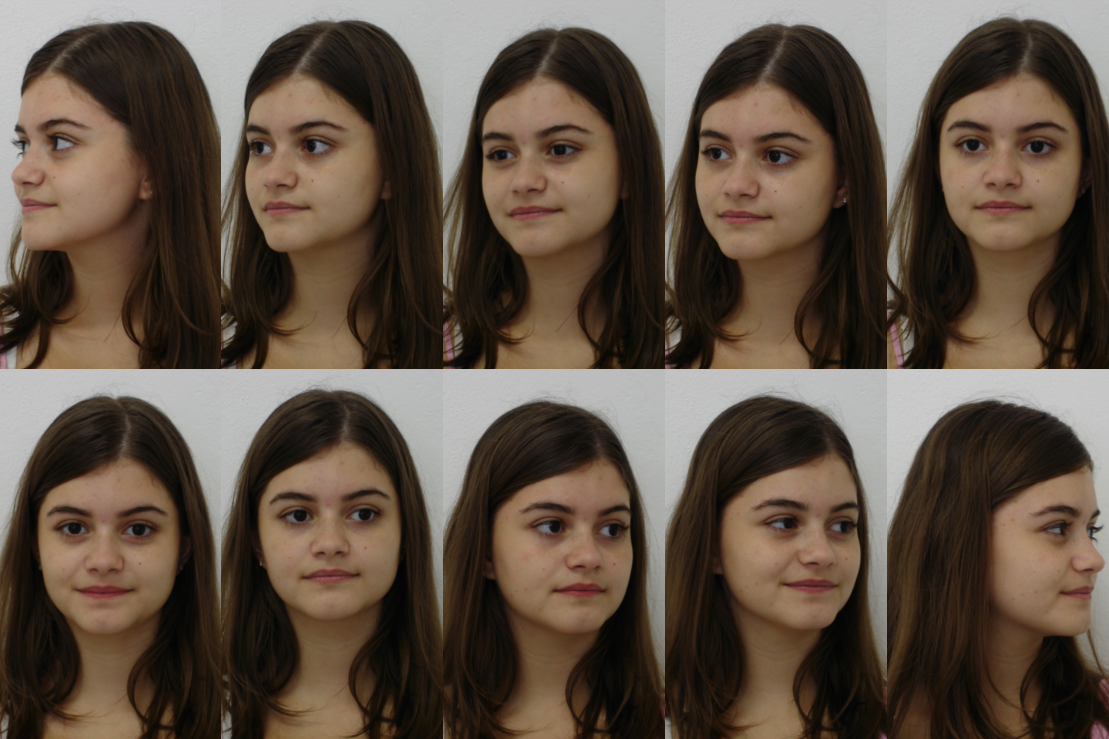
\includegraphics[width=150mm, keepaspectratio]{03_images/ori_all1.png}
    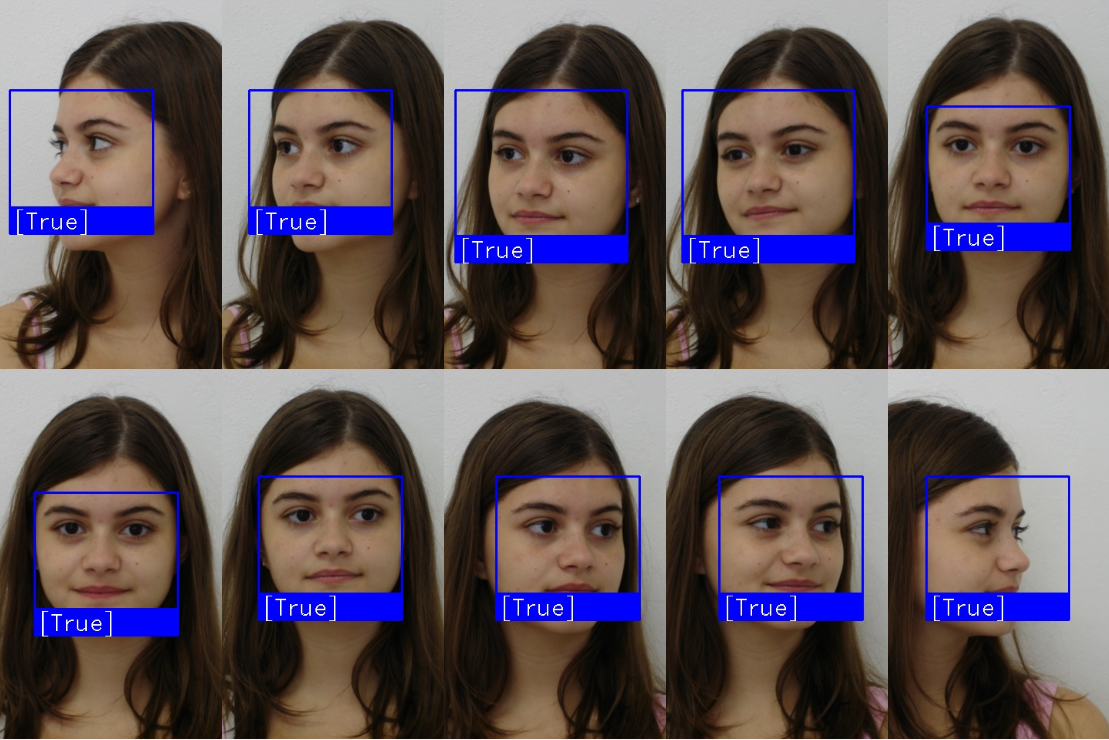
\includegraphics[width=150mm, keepaspectratio]{03_images/ori_all2.png}
	\caption{Arc több orientációban.}
	\label{fig:ori_test}
\end{figure}           % Mellékletek

\end{document}
